%\documentclass[abstract=on,a4paper]{scrreprt}
\documentclass[pdftex,10pt,b5paper,twoside]{book}
\usepackage[lmargin=25mm,rmargin=25mm,tmargin=27mm,bmargin=30mm]{geometry}

%\usepackage{a4wide}
\usepackage[utf8]{inputenc}
\usepackage{comment}
\usepackage{listings}
\usepackage{fancyvrb}
\usepackage[dvipsnames,table]{xcolor}
\usepackage[normalem]{ulem}
\usepackage{graphicx}
\usepackage{gensymb}
\usepackage{float}
\usepackage{pbox}
\usepackage[T1]{fontenc}
%------ Listings --------------
\usepackage{color}
\definecolor{light-gray}{gray}{0.95}
\definecolor{orange}{rgb}{1, 0.5, 0}
\usepackage{listings}

\lstnewenvironment{code}[1][]%
{\minipage{\linewidth}
\lstset{ %
language=C,  % choose the language of the code
basicstyle=\footnotesize,       % the size of the fonts that are used for the code
numbers=left,                   % where to put the line-numbers
numberstyle=\footnotesize,      % the size of the fonts that are used for the line-numbers
stepnumber=1,                   % the step between two line-numbers. If it is 1 each line will be numbered
resetmargins=true,              % reset line numbers
numbersep=5pt,                  % how far the line-numbers are from the code
backgroundcolor=\color{white},  % choose the background color. You must add \usepackage{color}
showspaces=false,               % show spaces adding particular underscores
showstringspaces=false,         % underline spaces within strings
showtabs=false,                 % show tabs within strings adding particular underscores
frame=single,                   % adds a frame around the code
tabsize=2,                      % sets default tabsize to 2 spaces
captionpos=b,                   % sets the caption-position to bottom
breaklines=true,                % sets automatic line breaking
breakatwhitespace=false,        % sets if automatic breaks should only happen at whitespace
escapeinside={\%*}{*)},         % if you want to add a comment within your code
identifierstyle=\color{blue},
stringstyle=\color{orange},
#1
}}%
{\endminipage}

%-------For showing code snippets-----------
\usepackage{xcolor} % for setting colors

% set the default code style
\lstset{
    frame=tb, % draw a frame at the top and bottom of the code block
    tabsize=4, % tab space width
    breaklines=true,
    showstringspaces=false, % don't mark spaces in strings
    numbers=left, % display line numbers on the left
    commentstyle=\color{green}, % comment color
    keywordstyle=\color{blue}, % keyword color
    stringstyle=\color{red} % string color
}




\RecustomVerbatimCommand{\VerbatimInput}{VerbatimInput}%
{fontsize=\footnotesize,
 %
 frame=lines,  % top and bottom rule only
 framesep=2em, % separation between frame and text
 rulecolor=\color{Gray},
 %
 label=\fbox{\color{Gray}All commands executed during task 1.1.c)},
 labelposition=topline,
 %
 commandchars=\|\(\), % escape character and argument delimiters for
                      % commands within the verbatim
 commentchar=*        % comment character
}
\Verba




\usepackage[pagestyles]{titlesec}
\usepackage{hyperref}
\usepackage{datetime}
\usepackage{amssymb} 
\usepackage[toc,page]{appendix}
\usepackage[final]{pdfpages}
\usepackage{array} % for defining a new column type
\usepackage{varwidth} %for the varwidth minipage environment
%\usepackage[table]{xcolor}
%\usepackage{amsmath}
\usepackage{mathtools}
%\titleformat{\chapter}[display]{\normalfont\bfseries}{}{0pt}{\Huge}
\usepackage{gensymb}

\usepackage[export]{adjustbox}
\usepackage{graphics}
\usepackage{array}
\usepackage{rotating}
\usepackage{tikz}
\usepackage{subfig}
\usepackage{mwe}
\usepackage{caption}
\usepackage{subcaption}
\usepackage{amsmath}

\usepackage{datatool}% http://ctan.org/pkg/datatool
\newcommand{\sortitem}[1]{%
  \DTLnewrow{list}% Create a new entry
  \DTLnewdbentry{list}{description}{#1}% Add entry as description
}
\newenvironment{sortedlist}{%
  \DTLifdbexists{list}{\DTLcleardb{list}}{\DTLnewdb{list}}% Create new/discard old list
}{%
  \DTLsort{description}{list}% Sort list
  \begin{itemize}%
    \DTLforeach*{list}{\theDesc=description}{%
      \item \theDesc}% Print each item
  \end{itemize}%
}

\date{September 2017}


\setcounter{tocdepth}{4}
\setcounter{secnumdepth}{4}

\newdateformat{monthyeardate}{%
  \monthname[\THEMONTH], \THEYEAR}


\begin{document}
%% Frontpage... DAIM will automatically gernerate a front page 

%Begin first page
%\begin {center}
%
\includegraphics[height=1in,keepaspectratio]{images/ntnu_logo.pdf}
%\centering
%
%\vspace*{5\baselineskip}
%\LARGE FPGA Implementation of Hyperspectral Anomaly  \\
%Detection Algorithm\\
%
% 
%\normalfont
%\small
%\vspace*{5\baselineskip}
%\textbf{by}\\
%\textbf{Martin Haukali\\
%\monthyeardate\today \\
%}
%\vspace*{5\baselineskip}
%\LARGE Master thesis
%
%\normalfont
%\small
%\vspace*{1\baselineskip}
%Department of Electronic Systems \\
%Norwegian University of Science and Technology
%\vspace*{1\baselineskip}
%
%\vspace*{3\baselineskip}
%\begin{flushleft}
%
%Co-supervisor: Professor Kjetil Svarstad \\
%Supervisor: Postdoctoral fellow Milica Orlandic \\
%
%
%\end{flushleft}
%\vspace*{3\baselineskip}
%
%%INSERT YOUR NAME HERE
%
%
%
%   
%\end {center}
%end first page
\thispagestyle{empty}
\newpage
\pagenumbering{roman}
\newpage

\Huge{\textbf{Project Assignment}}
\\
\\
\\
\small
\textbf{Candidate name: }  Martin Haukali
\\
\\
\\
\textbf{Assignment title:}  FPGA Implementation of Hyperspectral Anomaly Detection Algorithm
\\
\\
\textbf{ Assignment text: }
This topic is part of the large project Hyperspectral Imaging in Small Satellites. Hyperspectral imaging relies
on sophisticated acquisition and on data processing of hundreds or thousands of image bands. Most of the
algorithms for hyperspectral imaging perform intensive matrix manipulations, and
FPGAs are recommended to be used due to reconfiguration, low consumption, compact size and high
computing power.

Anomaly detection is an important task for hyperspectral data exploitation.
A standard approach for anomaly detection in the literature is the method called RX algorithm.
The computational cost is very high for RX algorithm and current advances
in high performance computing can be good solution to reduce the run- time of this algorithm.\\

Tasks:\\
- Optimization of RX algorithm for parallel processing\\
- Covariance computation\\
- Hardware implementation of inverse matrix problem\\
- FPGA implementation of RX algorithm \\


\textbf{Supervisor:  }Kjetil Svarstad 
\\
\\
\textbf{Co-supervisor: }Milica Orlandic

\newpage
%% Answer the following questions
%\section{Abstract}
\begin{abstract}

What is all this about?
\\
Why should I read this thesis?
\\
Is it any good?
\\
What's new?
%\\





\end{abstract}

\newpage
\chapter*{Preface}
% Here you can describe the process that led to the writing of this report (i.e., the project work process). Here you can mention why you chose this assignment and specific challenges you met with during your work. You can also thank people for help and support during this project.
%% Answer the following questions
%Have you done anything that doesn't have to do with your research?
%\\ Have you published parts of this work before?

%%% ACKNOWLEDGEMENT %%%
%Who is your advisor?
%\\
%Did anyone help you?
%\\
%Who funded this work?
%\\
%What's the name of your favourite pet?



This thesis is submitted to the department of Electronics Systems at NTNU as part of the Master of Science degree in Electronics, with specialization in digital circuit design. The project is part of the SmallSat project at NTNU, a resarch project at NTNU which is focused on the design and creation of small satellites. The project was started on in the mid of January. 
\\

The purpose of this thesis is to design an Anomaly detector in hardware, to be implemented on a Field-Programmable Gate array. 
\\


Thanks to Milica Orlandic for great guidance and help during the semester.

%I would like to thank my supervisors; Håvard Tørring and Professor Snorre Aunet for guidance and help throughout the semester. A special thanks to Disruptive Technologies for providing the funds necessary to buy development kits and other equipment used in this project. I would also like to specially thank Postdoctoral Fellow Milica Orlandic for helping me with image compression for FPGAs, and for giving me an Intellectual Property for Sobel Edge detection, and for providing me with a testbench to test the design. \\

%It is assumed that the reader has some basic knowledge in electronics and digital circuits.
\newpage
\tableofcontents
\listoffigures
 
\listoftables
 




%\section{List ofAbbreviations}
\chapter*{List of Abbreviations}





\begin{sortedlist}
  \sortitem{IP -    Intellectual Property}
  \sortitem{FPGA -  Field Programmable Gate Array}
  \sortitem{HSI - Hyperspectral imaging}
  \sortitem{RX - Reed-Xiaoli}
  \sortitem{LRX - Local RX}
  \sortitem{AD - Anomaly detector}
  \sortitem{ACAD - Adaptive Causal anomaly detection}
  \sortitem{HAB - Harmful algae bloom}
  \sortitem{CORDIC - Cordinate Rotation Digital Computer} 

  \end{sortedlist}
 
\thispagestyle{empty}

\newpage
\pagenumbering{arabic} 
\newpage
%\section{Introduction}
\chapter{Introduction}
\label{sec:introduction}
\section{Motivation}

This master thesis is part of the NTNU SmallSat \cite{SmallSat_project_description} project. The projects mission is to use hyperspectral imaging to observe ocean color in the ocean and the coast of Norway. The payload of the satellite will be a 1/3 U push-broom type hyperspectral imager (HSI), dedicated to take images of a $30x30 km^2$. In regular Red Green Blue(RGB) imaging each of the image pixels is made up of three frequency components that represent the intensities in red, green and blue frequencies respectively. Such a component is referred to as a band. In hyperspectral imaging, a pixel will typically consists of hundreds to thousands of bands, providing more information than regular images. This information can be used for a lot of different purposes. It can for example be used to detect different materials in an area, by using spectral signatures of materials as identifiers. This is shown in Figure \ref{fig:HSI_concept}.\\

\begin{figure}[H]
\centering
   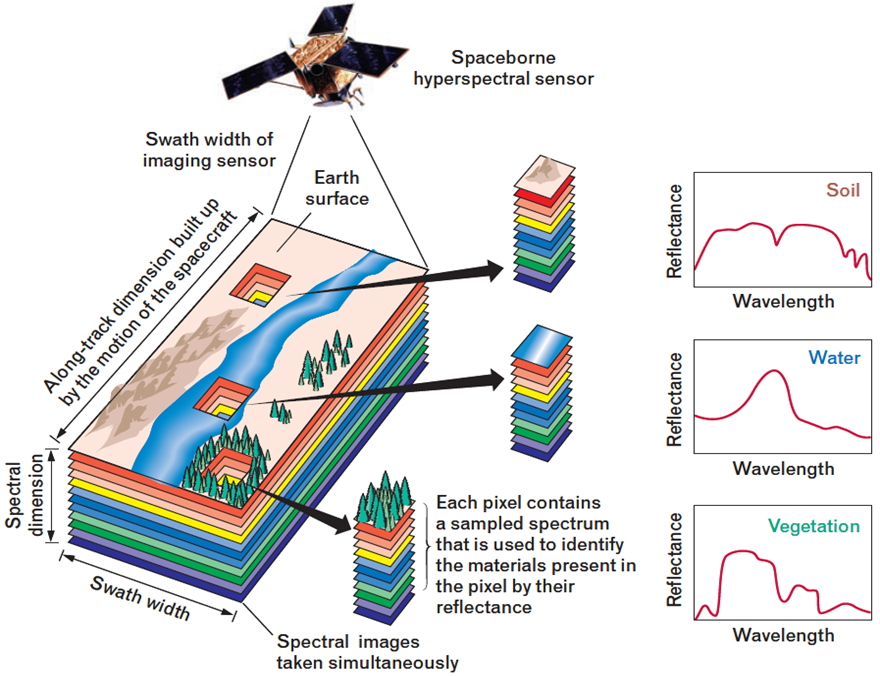
\includegraphics[scale=0.3]{images/Imaging-Spectroscopy-Concept.png}
  \caption{ Functional concept of HSI.\cite{HSI_concept} } 
  \label{fig:HSI_concept}
\end{figure}


NTNU SmallSat aims to use this information to detect algae blooms, phytoplankton and possibly other irregularities or \textit{anomalies} in the ocean. Detection of algae blooms is particularly interesting for the salmon farms located along the coast of Norway, as such blooms can be toxic, even deadly, for the salmon. Algaes were most likely the cause of death for 38 000 salmons in southern Troms in September of 2017 \cite{laksedeath}. An image of such a bloom can be seen in Figure \ref{fig:algae_bloom_troms}.  %With the increasing rise in sea temperatures and the issues faced with global warming this is an even 
% HSI  = hyperspectral imager or imaging?
\\

\begin{figure}[H]
\centering
   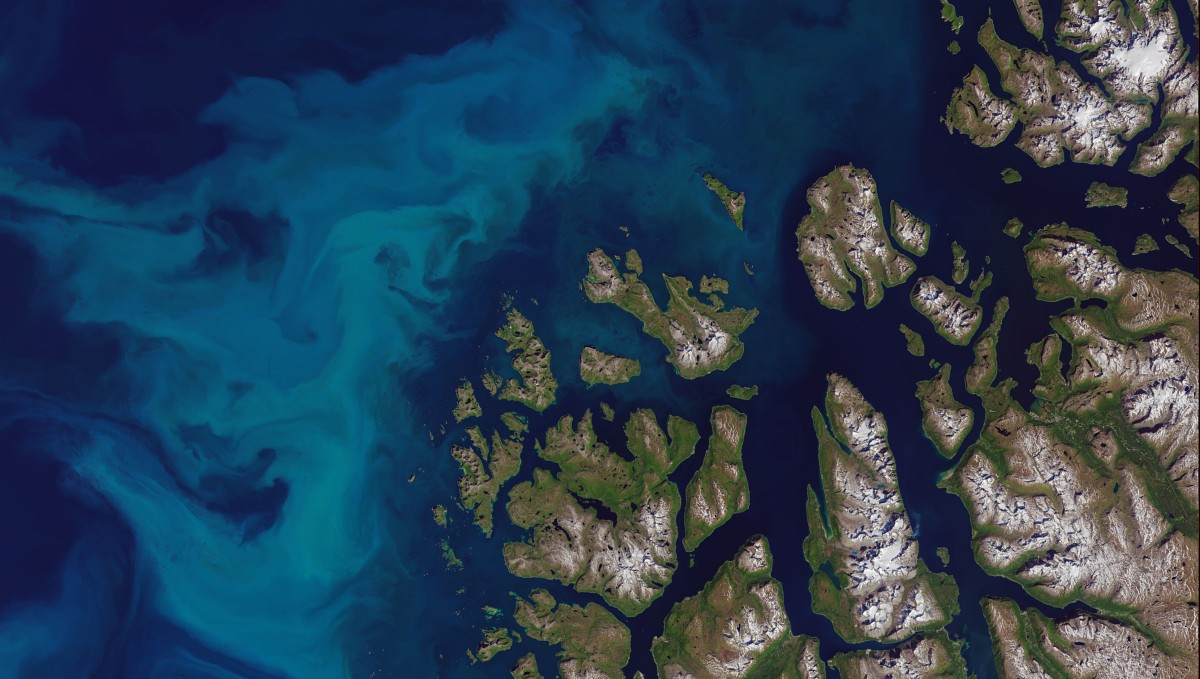
\includegraphics[scale=0.3]{images/algaes/algaes_northern_troms.jpg}
  \caption{ Image of an algae bloom along the coast of Troms in Norway \cite{laksedeath}. Foto by NASA EARTH OBSERVATORY. } 
  \label{fig:algae_bloom_troms}
\end{figure}
\\

Algaes will have spectral signature that is different to the background, which will be ocean water or land. It may therefore be considered an \textit{anomaly}. An anomaly in the context of HSI is a pixel vector that have significant spectral differences from its surrounding background pixels \cite{yang2015dual}.  
\\
As hyperspectral images contain a lot of data, and the transmission time is short(*Something something transmission while over area*, reaction time...)
 
 





\newpage
\subsection{Project report overview}
The following chapters in this project report delve into the design of a miniature camera on the Disruptive Technology sensor platform. Different image sensors will be considered, with respect to design parameters such as size, battery lifetime, energy, power dissipation and area of application. Three different system alternatives with different system partitioning are analyzed and evaluated. One system is proposed for implementation.\\  

Chapter \ref{sec:theory} is the Theory section. 


Chapter \ref{sec:methodology} is the Methodology section. 


Chapter \ref{sec:results} is the Results section. Results from estimations of energy consumption, battery-capacity consumption and power dissipation are presented here based on methodology presented in chapter \ref{sec:methodology}. Also, experimental results from doing image processing on pictures taken with the NanEye2D image sensor are presented here. 
\\

Chapter \ref{sec:Discussion} is the Discussion section. The results of the energy and power estimations for the three system alternatives are discussed here. A comparison of the different alternatives is made based on metrics such as number of frames possible to capture, process and transmit, area of application and compression rate possible. 
\\

Chapter \ref{sec:conclusion} is the Conclusion section. The most important results are presented here. The proposed system of the miniature camera is presented as well. Future work that can be done is mentioned, listed in bullet-points. 
\\






\newpage
%\section{Background Theory}
\chapter{Background Theory}
\label{sec:theory}

%\newpage
%\section{Applications}
\chapter{Applications}
\label{sec:applications}
\section{Use cases}
\newpage 
%\section{Methodology}¨
%\chapter{Methodology}
%\label{sec:methodology}

\chapter{Review of state of the art anomaly detectors}
%\section{Evaluation of RX, LRX and ACAD }
%\label{sec:MATLAB_methodology}
\label{chapter:review_anomaly_detectors}
To evaluate the performance of the ADs considered in this task, models of the algorithms described in section \ref{sec:anomaly_detectors_theory} were developed in MATLAB, and tested on both hyperspectral image data from the Cuprite site \cite{Cuprite_data} taken by NASA's AVIRIS hyperspectral imager and synthetic images created by the author. 
\\

The MATLAB hyperspectral toolbox \cite{MATLAB_hyperspectral_toolbox} was used for image preprocessing, visualization and for having a good starting point for developing further functionality. The toolbox included an implementation of the RX algorithm. A fork of the toolbox was made, available at \cite{MATLAB_hyperspectral_toolbox_fork}, to be able to do MATLAB implementations of LRX, ALRX and ACAD in order to evaluate the performance of the ADs. The most important scripts and functions from the forked toolbox are also located in appendix \ref{appendice:MATLAB_hyperspectral}.
\section{Experiments on Synthetic images testing}
To make an objective analysis  of the considered ADs performance, synthetic hyperspectral images with known anomalies were created. The images contained anomalies of various sizes, to test the test-ADs ability to detect variably sized anomalies. A similar test is also done in \cite{global_and_local_rx}. Figure 7(a) in \cite{global_and_local_rx} shows that the RX algorithm was not able to detect anomalies in the third and four column (anomalous pixels made up of >50\% abundance of the anomaly signature). The LRX exhibit slightly better anomaly detection accuracy in this test.
\\

The purpose of the synthetic images used in this thesis was to get objective metrics of the performance of the evaluated ADs. Two different metrics are important in order to evaluate the performance of the ADs; $false\_anomalies$ and $\%correctly\_predicted\_anomalies$. These metrics are defined in equation \ref{eq:false_anomalies_metric} and \ref{eq:correctly_predicted_anomalies_metric}. The value $true\_anomalies$ is taken from the reference anomaly map created during the creation of the synthetic images. These values are important as they provide an objective metric to evaluate the performance of the ADs, something that can not be done with real hyperspectral image data, unless one posesses a reference anomaly map to the real image data, which the author has not been able to find.  

% If this is bigger than >0, else 0
\begin{equation}
    false\_anomalies = predicted\_anomalies - true\_anomalies
    \label{eq:false_anomalies_metric}
\end{equation}


\begin{equation}
    \%correctly\_predicted\_anomalies= \frac{predicted\_anomalies-false\_anomalies}{true\_anomalies}
    \label{eq:correctly_predicted_anomalies_metric}
\end{equation}

Synthetic images with different image size and size of anomaly were created to evaluate the performance of the ADs. To be able to compare to the tests done on images with a size of 200x200 as described in chapter 5.5.1 in \cite{hsueh_master_thesis} by Hsueh, these tests were mimicked. The synthetic image can be seen in figure \ref{fig:hsueh_image}. In addition, synthetic images with size of 30 x 30 pixels were created with an anomalous panel of size 2x2 inserted into the center of the images. This image scene is labelled as $Sim30\_30AVIRIS$. The anomalous pixels are pure pixels with a spectral signature of Buddingtonite. These images has a background consisting of $33\%$ Alunite, $33\%$ Kalonite and $33\%$ Pyrope, extracted from the Cuprite image scene \cite{ground_truth_cuprite}. Such a generated synthetic image can be seen in Figure \ref{fig:synthetic_30_30}.


\begin{figure}[H]
\begin{minipage}[]{.5\linewidth}
\centering
\subfloat[ 200 x 200 synthetic image.]{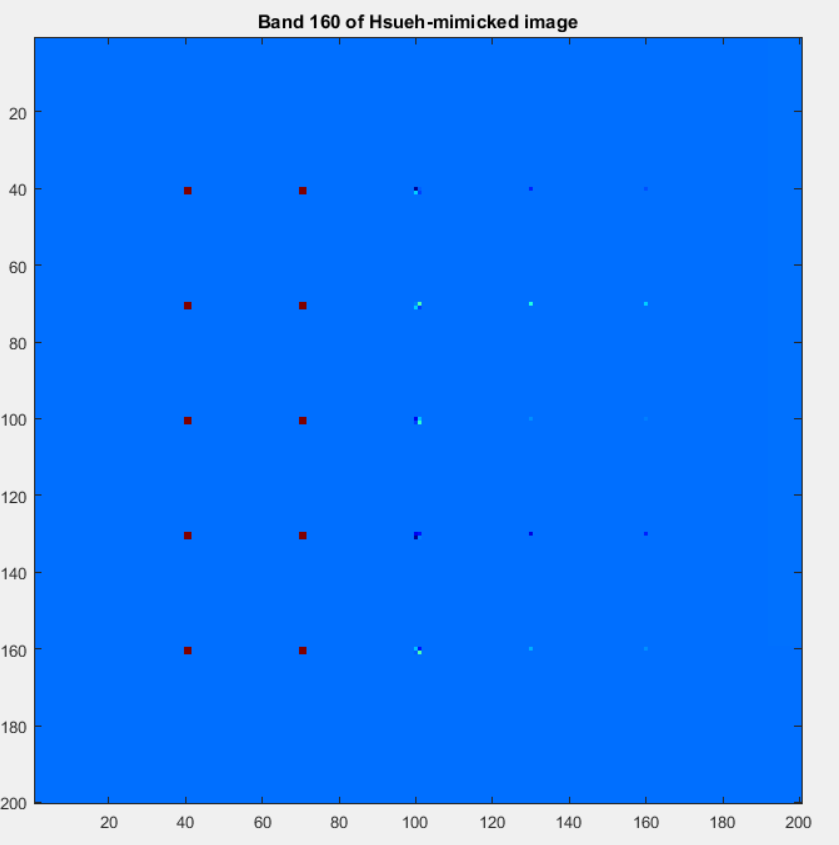
\includegraphics[scale=.5]{images/AD_testing/synthetic_images/band_160_hsueh_picture_without_gaussian_noise.PNG}}
  %\caption{Lena 256 x 256 uncompressed. Used for testing of MATLAB SPIHT script.}
  %\label{fig:lena_unc}
\end{minipage}%
\begin{minipage}[]{.5\linewidth}
\centering
  \subfloat[Synthetic image with added Gaussian white noise with a SNR of 20:1.]{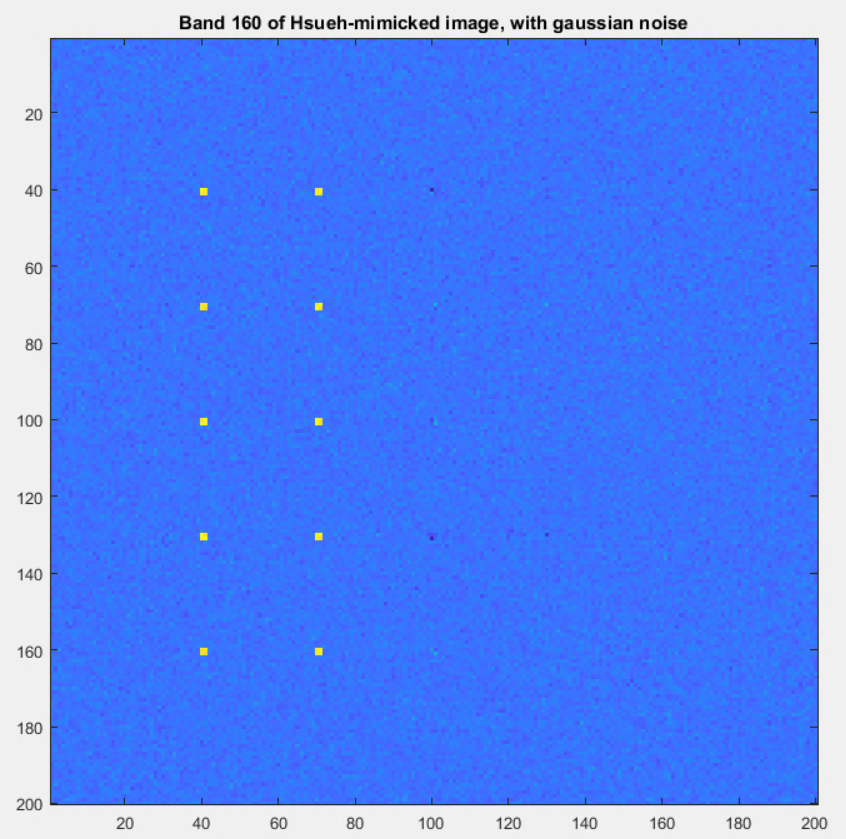
\includegraphics[scale=.5]{images/AD_testing/synthetic_images/band_160_hsueh_picture_with_gaussian_noise.PNG}}
  %\caption{Lena 256 x 256 reconstructed after being compressed having 0.1 bpp, using the MATLAB SPIHT script. See appendix. }
  %\label{fig:lena_comp}
\end{minipage}


\caption{First class of synthetic images: 200 x 200 synthetic image with 25 inserted anomaly panels as describe by Hsueh in \cite{hsueh_master_thesis}. Displaying spectral band 160. }
\label{fig:hsueh_image}
\end{figure}

\begin{figure}[H]
\centering
   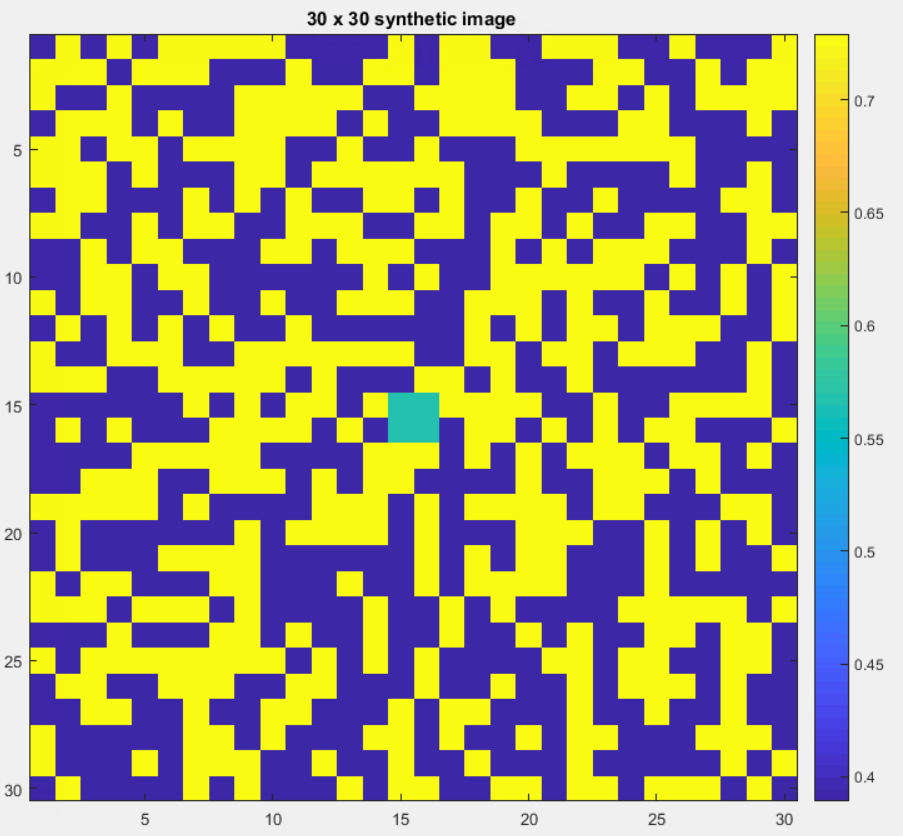
\includegraphics[scale=0.4]{images/AD_testing/synthetic_images/30_30_anomaly_image.PNG}
  \caption{Second class of synthetic images: Synthetic 30x30 image with an inserted 2x2 anomalous panel inserted into the center. Displaying band 160. } 
  \label{fig:synthetic_30_30}
\end{figure}


\\
A third class of synthetic images with a size of $100$ x $614$ pixels was also created. These images had a background consisting of $33\%$ Alunite, $33\%$ Kalonite and $33\%$ Pyrope. The anamalous pixels are pure pixels with a spectral signature of Buddingtonite, extracted from the Cuprite image scene \cite{ground_truth_cuprite}. Six different sized anomalous-target kernels were made, with a size of $1x1$, $2x2$, $5x5$, $10x10$, $15x15$, $20x20$ and $25x25$ pixels.




\begin{table}[H]
\centering
\caption{Properties of the third class of synthetic images used in experiments. Row and column locations are location of the center pixel in the kernel of size $k x k$.}
\label{tab:synthetic_images}
\begin{tabular}{l|l|l|l}
\textbf{Scene} & \textbf{Row} & \textbf{Column} & \textbf{Anomaly size {[}pixels x pixels{]}} \\
SimAviris01    & 35           & 50              & 1x1                                         \\
SimAviris01    & 70           & 50              & 1x1                                         \\
SimAviris01    & 35           & 100             & 2x2                                         \\
SimAviris01    & 70           & 100             & 2x2                                         \\
SimAviris01    & 35           & 150             & 5x5                                         \\
SimAviris01    & 70           & 150             & 5x5                                         \\
SimAviris01    & 35           & 250             & 10x10                                       \\
SimAviris01    & 70           & 250             & 10x10                                       \\
SimAviris01   & 35           & 350             & 15x15                                       \\
SimAviris01    & 70           & 350             & 15x15                                       \\
SimAviris01    & 35           & 450             & 20x20                                       \\
SimAviris01    & 70           & 450             & 20x20                                       \\
SimAviris01    & 35           & 550             & 25x25                                       \\
SimAviris01    & 70           & 550             & 25x25                                      
\end{tabular}
\end{table}



\begin{figure}[H]
\hbox{\hspace*{-0}                                              
   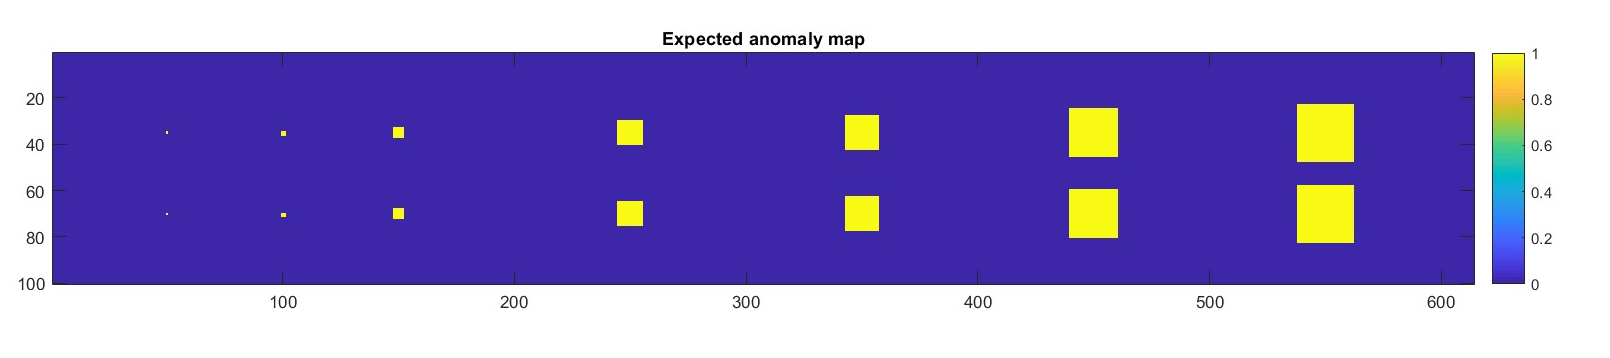
\includegraphics[scale=0.4]{images/AD_testing/synthetic_images/expected_anomaly_map.png}}
  \caption{Expected anomaly map for the third class of synthetic images created.} 
  \label{fig:anomaly_map_615_100}
\end{figure}

\subsection{RX}


\subsubsection{Hsueh-mimicked image}

\begin{figure}[H]
\begin{minipage}[]{.5\linewidth}
\centering
\subfloat[ RX AD result for synthetic image shown in \ref{fig:hsueh_image}. ]{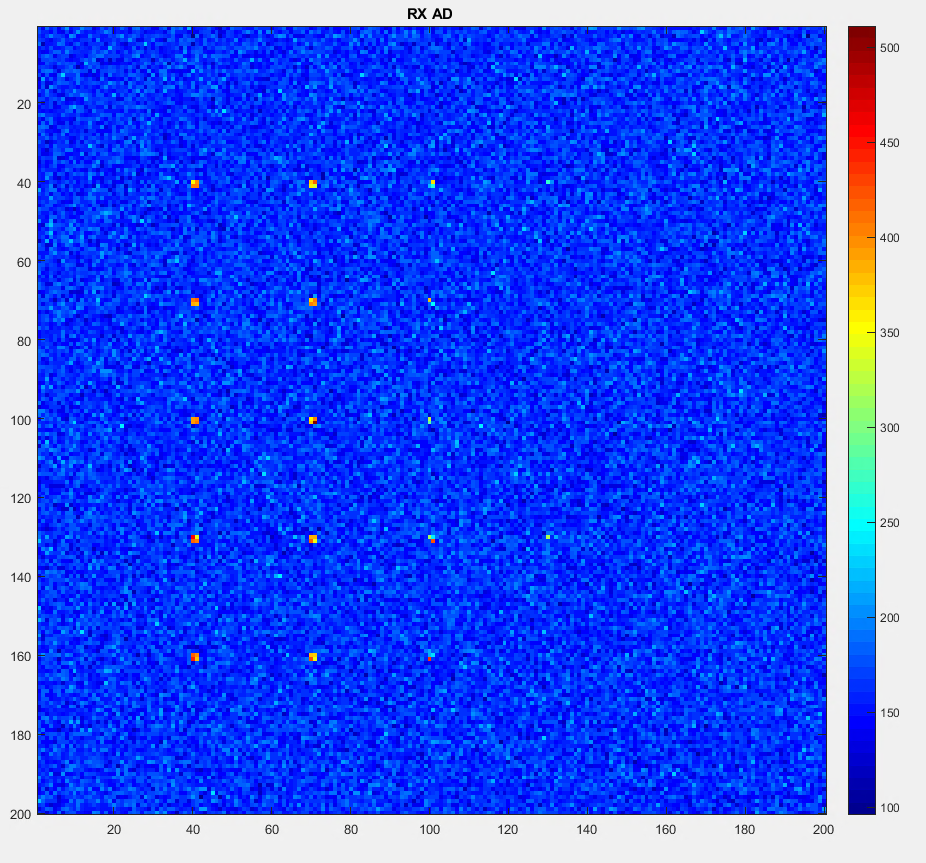
\includegraphics[scale=.35]{images/AD_testing/synthetic_images/rx_ad_hshueh.PNG}}
  %\caption{Lena 256 x 256 uncompressed. Used for testing of MATLAB SPIHT script.}
  %\label{fig:lena_unc}
\end{minipage}%
\begin{minipage}[]{.5\linewidth}
\centering
  \subfloat[Generated anomaly map for RX, setting threshold value for what is considered an anomaly as $\geqslant$ 75\% of the max value of the RX AD.]{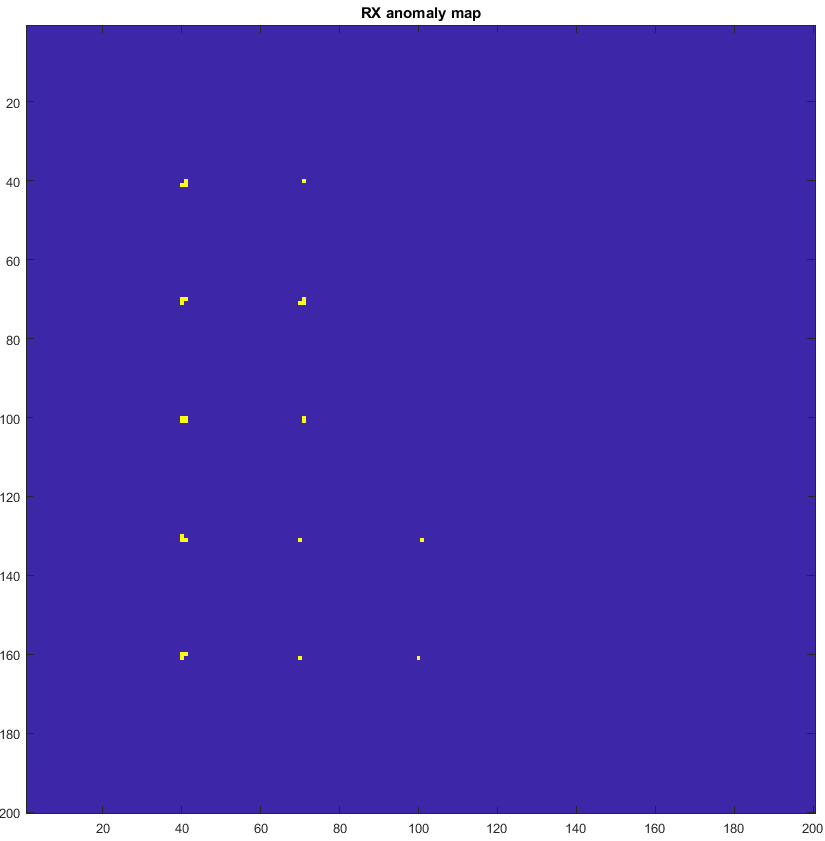
\includegraphics[scale=.3]{images/AD_testing/synthetic_images/rx_hsueh_anomaly_map.PNG}}
  %\caption{Lena 256 x 256 reconstructed after being compressed having 0.1 bpp, using the MATLAB SPIHT script. See appendix. }
  %\label{fig:lena_comp}
\end{minipage}


\caption{RX AD test on synthetic image based on Hsueh's description. The map in (b) was created to provide a way of computing $false\_anomalies$ and $ \%correctly\_predicted\_anomalies$.  }
\label{fig:hsueh_image}
\end{figure}

The value of $false\_anomalies$ = 0, and  $\%correctly\_predicted\_anomalies$ = $0.3714$ for this test.

\subsubsection{$Sim30\_30AVIRIS$ scene }




\subsection{LRX}

\subsection{ALRX}

\subsection{ACAD}


\section{Testing on data from real images}
To evaluate the performance of the ADs considered in this task, models of the algorithms were developed in MATLAB, and tested on hyperspectral image data from 


 Band 220 from the Cuprite scene can be seen in figure \ref{fig:cuprite_scene_band_220}.

\begin{figure}[H]

\hbox{\hspace*{-2cm}                                                           

   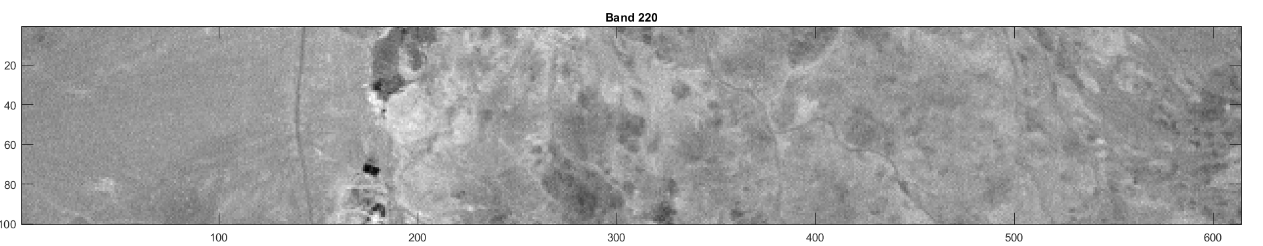
\includegraphics[scale=0.3]{images/AD_testing/original_band_220_22_1.png}}
  \caption{Spectral band 220 from the hyperspectral data set of the Cuprite site\cite{Cuprite_data}. } 
  \label{fig:cuprite_scene_band_220}
\end{figure}


\subsection{RX}
As described in section \ref{sec:RX_theory}, the RX algorithm computes the covariance on the global set of pixel vectors to indicate the probability of a pixel being an anomalous pixel. 

\begin{figure}[H]

\hbox{\hspace*{-2cm}                                                           

   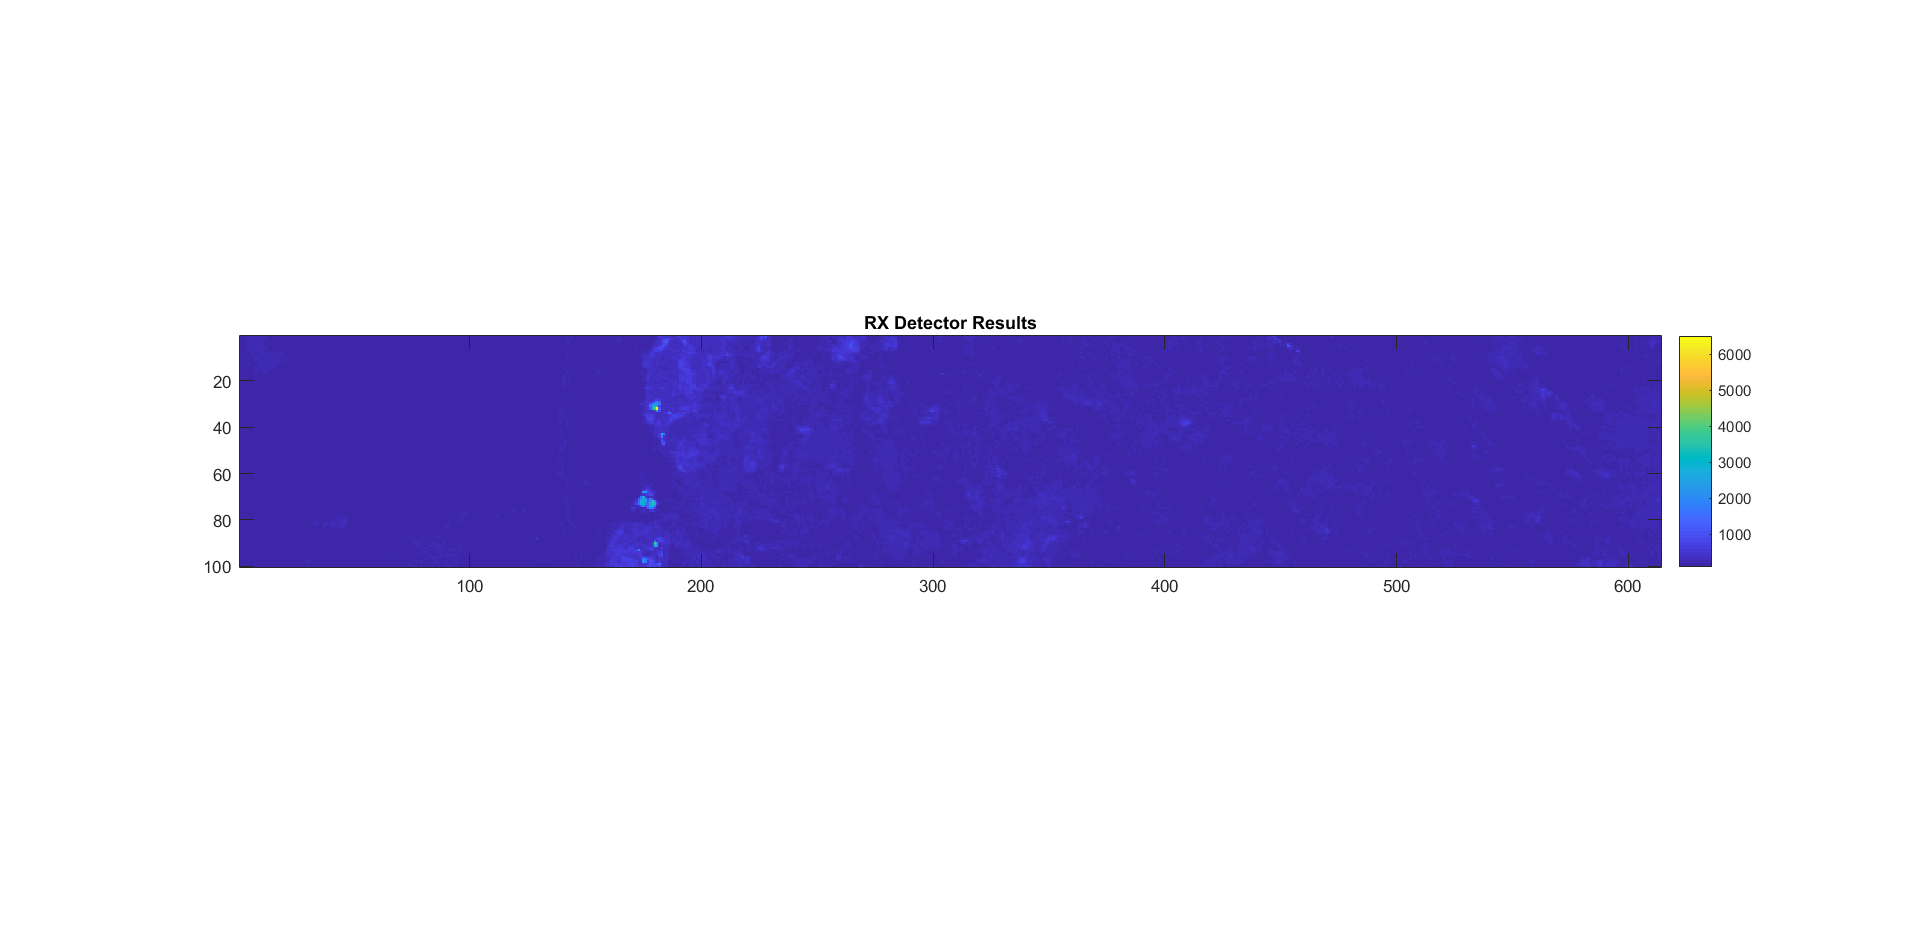
\includegraphics[scale=0.4]{images/AD_testing/GRX_22_1.png}}
  \caption{Result from RX AD on Cuprite image data. Higher score indicates higher probability of the pixel being anomalous. } 
  \label{fig:cuprite_scene_band_220}
\end{figure}


\subsection{LRX}
LRX computes the correlation matrix on a pixel vector block of size $K$ in order to detect anomalous pixel vectors, as described in section \ref{sec:LRX_theory}. 

\begin{figure}[H]

\hbox{\hspace*{-2cm}                                                           

   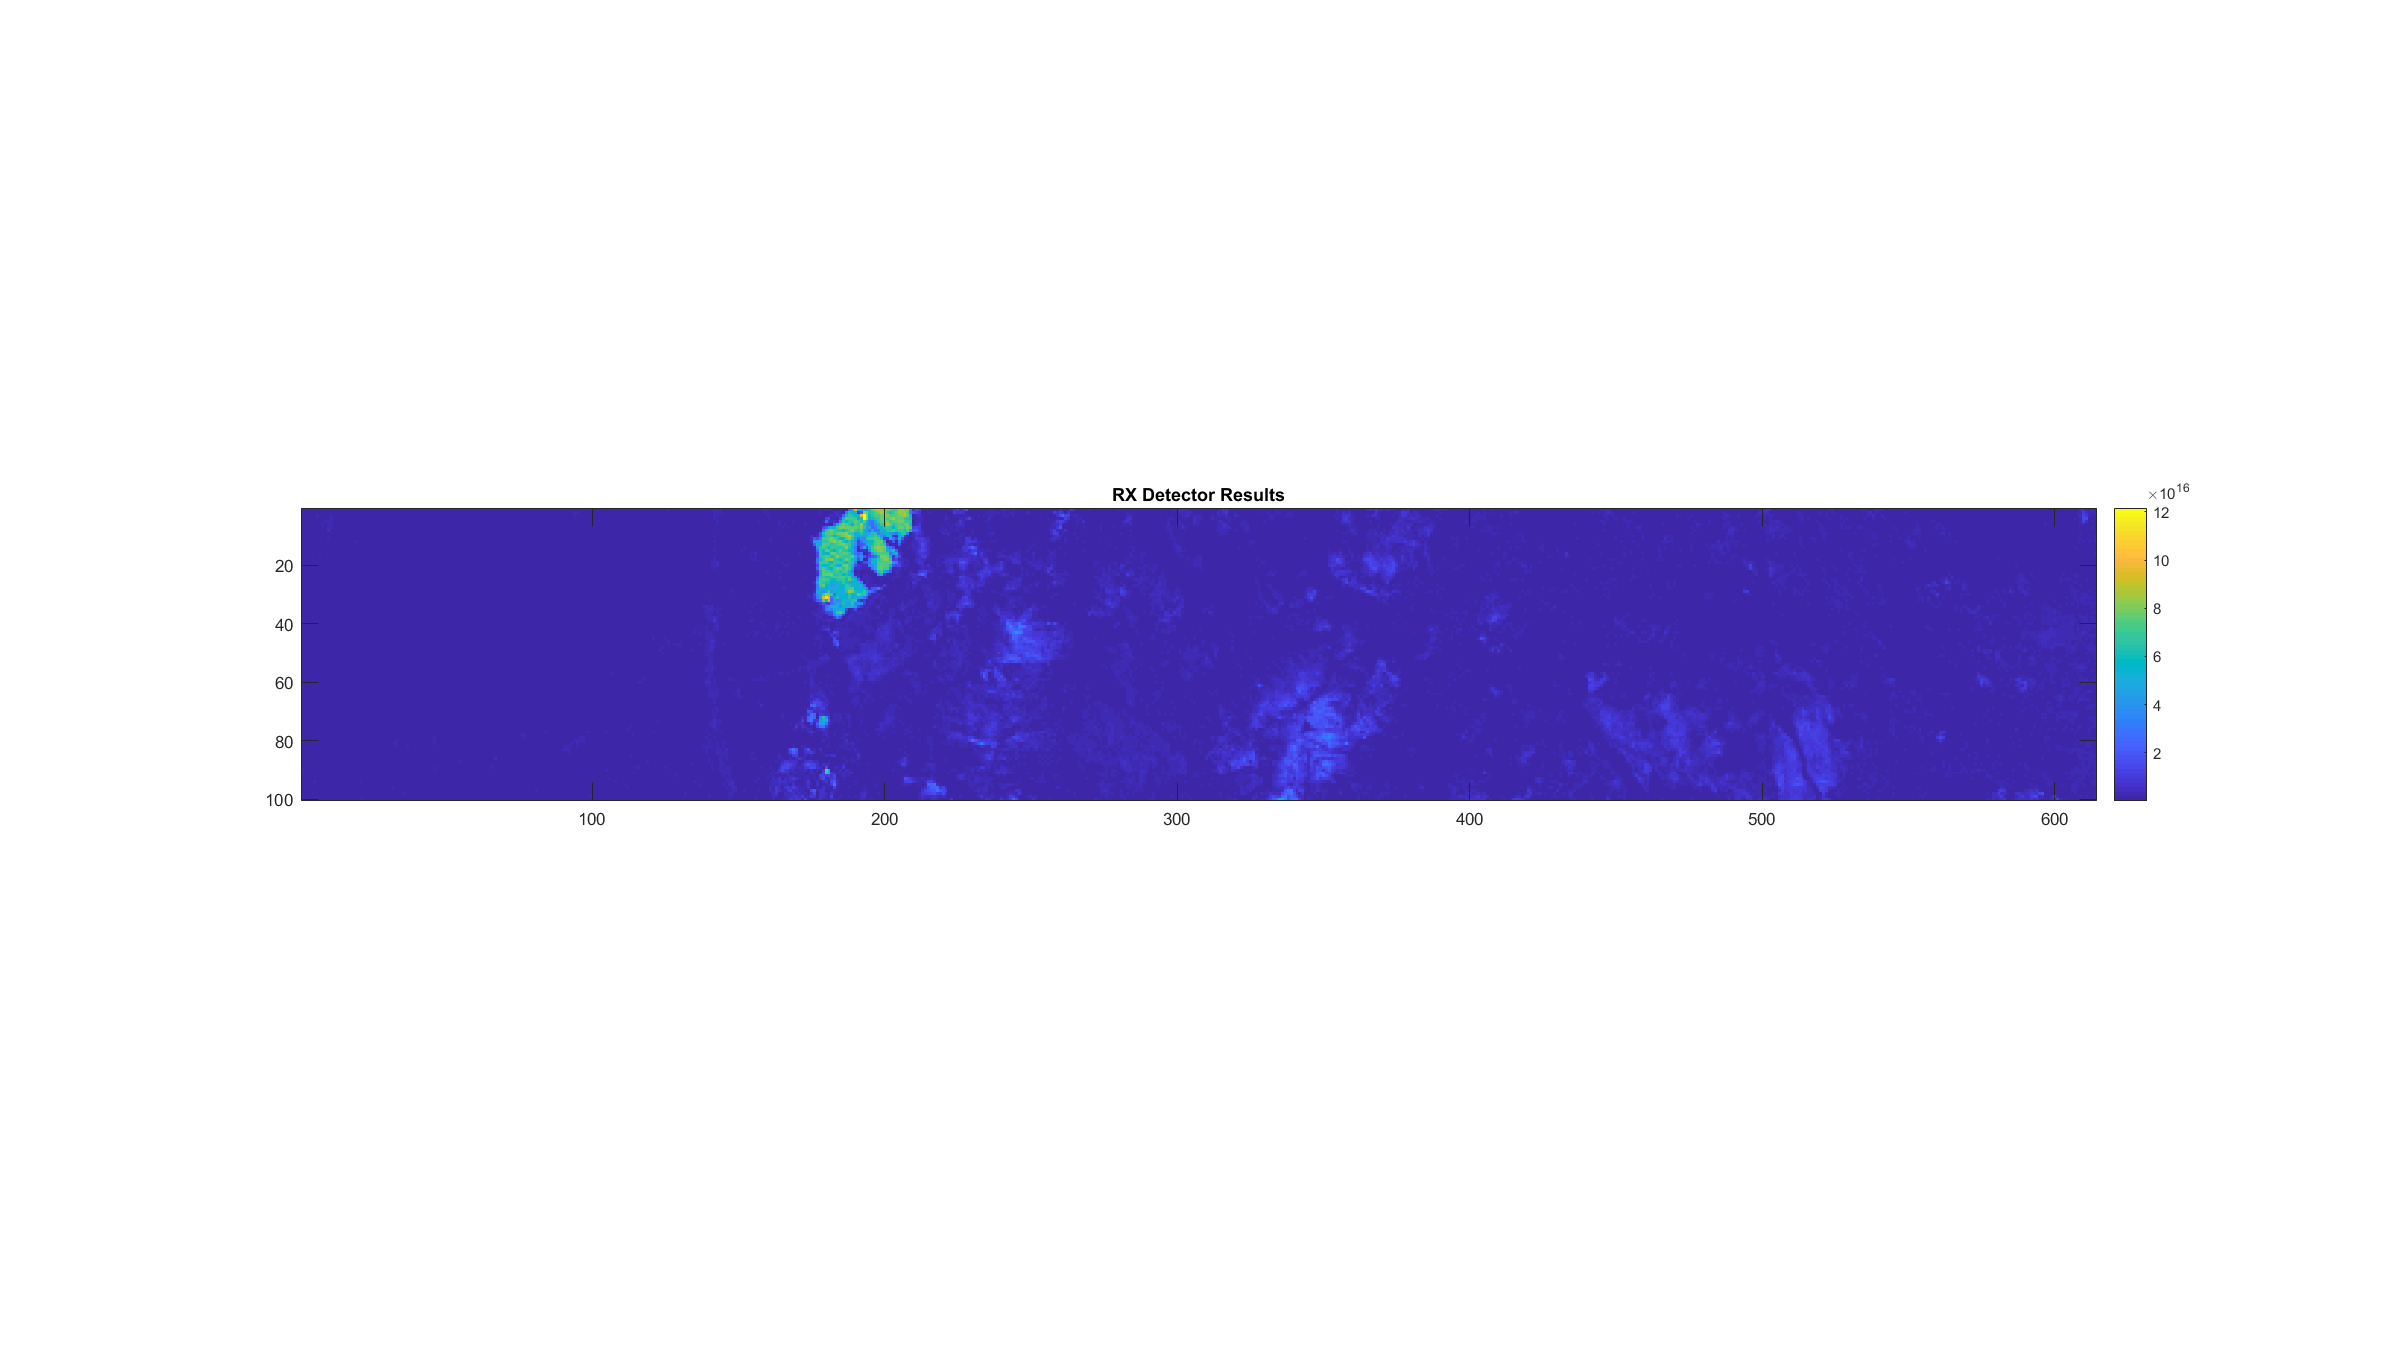
\includegraphics[scale=0.3]{images/AD_testing/K=23.png}}
  \caption{Result from LRX AD with a kernel size of K=23 on Cuprite image data. Higher score indicates higher probability of the pixel being anomalous. } 
  \label{fig:cuprite_scene_band_220}
\end{figure}


\subsection{ACAD}

ACAD is causal and computes the correlation matrix on a casual data set, back to the $N_{acad}$ previous pixel. This is further described in section \ref{sec:ACAD_theory}.

\begin{figure}[H]
\centering                                                           

   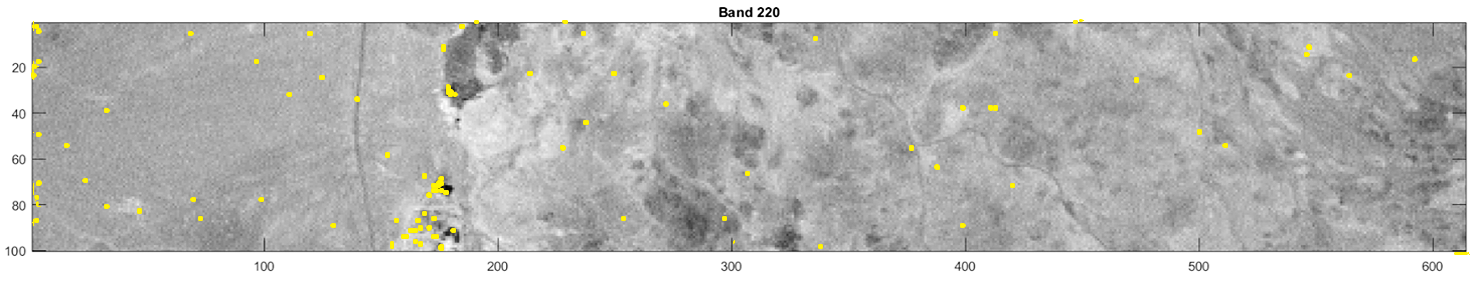
\includegraphics[scale=0.3]{images/AD_testing/anomaly_map_over_picture_tresh=250.png}
  \caption{Anomaly map created by ACAD( yellow dots) overlayed over Figure \ref{fig:cuprite_scene_band_220}. $\tau$ is set to 250.} 
  \label{fig:cuprite_scene_band_220}
\end{figure}
 
\newpage
\chapter{Hardware implementation}
\label{sec:implementation}
The following chapter describes the implementation of the ACAD anomaly detector on a Zynq Z-7030 or Z-7035 device, used for the NTNU Smallsat project. \\

\section{Memory considerations}
\label{sec:memory_management}
    As the ACAD anomaly detector is to be implemented on a Zynq Z-7030 or Z-7035 device, care must be taken when designing, with respect to logic and memory usage.The hyperspectral image data inputted to the AD might have number of spectral bands, $P\_bands$ =$N\_bands$, depending upon if preprocessing steps such as Principel Component Analysis(PCA) is done on the image cube. Pixel data width per spectral band, $Pixel\_data\_width$ is 16-bit. The size of $P\_bands$ and $Pixel\_data\_width$ makes memory usage an important consideration.

\subsection{Storing and updating of matrices in ACAD }
\label{sec:mem_management_correlation_matrix}
The ACAD algorithm requires storage of the following matrices :$\textbf{R(x}_k)$, $\Tilde{\textbf{R}}(\textbf{x}_k)$ and $\sum_{t_j\in\Delta(k)}\textbf{t}_j\textbf{t}_j^T$. In addition the matrix $A$ and $A^{-1}$ used in Gauss-Jordan elimination shown in Figure \ref{fig:matrix_A_and} must be stored in memory. These are $P\_bands$ $\times$ $P\_bands$ sized matrices. 

\begin{figure}[H]
\centering                                                              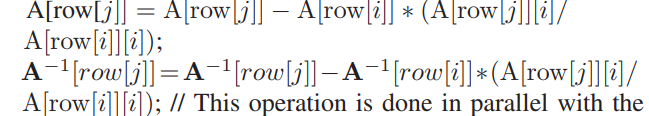
\includegraphics[scale=0.9]{images/matrix_A_and_inv.PNG}
  \caption{Matrix $A$ and $A^{-1}$ used in Gauss-Jordan elimination.} 
  \label{fig:matrix_A_and}.
\end{figure}

Storing and updating matrices of size $P\_bands$ $\times$ $P\_bands$  requires a lot of memory resources. %the causal correlation matrix sum as shown in equation \ref{eq:caus_corr} requires a lot of memory resources. 
One of the matrices is the causal correlation matrix $\textbf{R(x}_k)$. Update of this matrix needs to be done for each pixel in the image, and the memory used for this operation is therefore important in order to make the AD real-time.  As $\textbf{R(x}_k)$ is the product of $\textbf{x}$ $\times$ $\textbf{x}^T$ the resulting data width will be 2$\times$ $Pixel\_data\_width$. Using spectral information from all the bands would require $P\_bands$ $\times$ $P\_bands$ $\times$ $32$ $=$ $100$ $\times$ $100$ $\times$ $32$ bit = $320 kbit$ of memory storage. 
\\

There are three alternatives to storing all this information on the FPGA; storing it in block RAM, distributed RAM/LUTRAM or in registers. The FPGA to be used in the SmallSat's first prototype is the Zynq Z-7030 or the Zynq Z-7035. 
The FPGAs contains the memory resources as shown in figure \ref{fig:zynq_memory_resources}. The Z-7030 and the Z-7035 contains 265 and 500 36kbit BRAM blocks respectively. The number of DSP Slices is 400 for the Z-7030 and 900 for the Z-7035. These are important for implementation of multiplication. 





\begin{figure}[H]
\hbox{\hspace*{-1cm}                               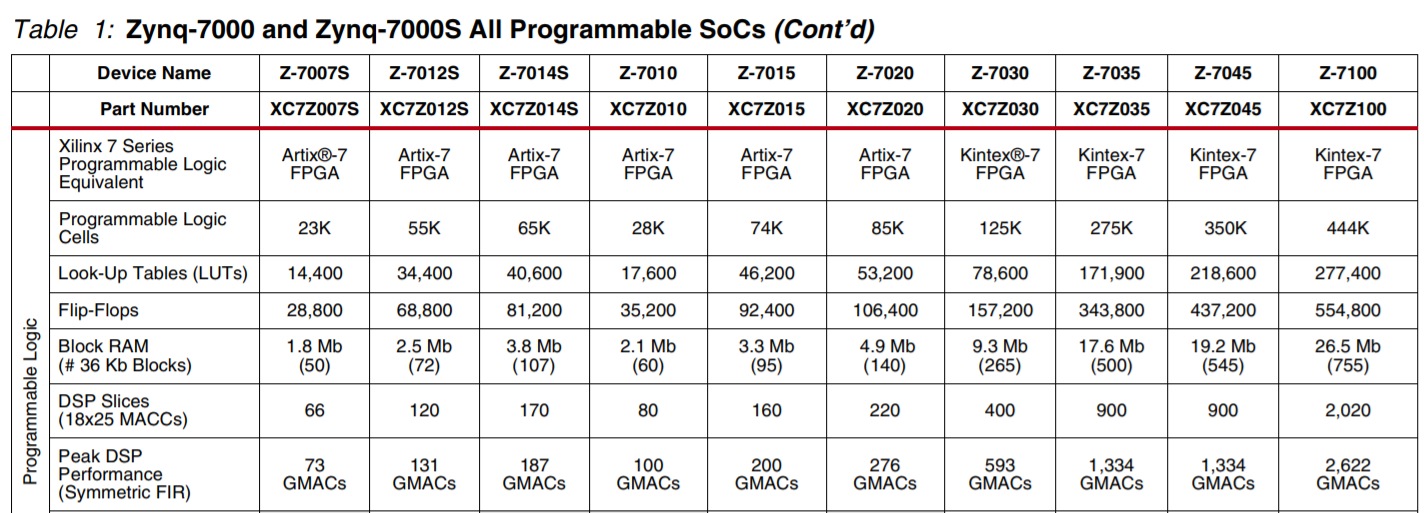
\includegraphics[scale=0.45]{images/zynq_memory_resources.PNG}}
  \caption{Zynq memory resources \cite{cite:mem_resources_zynq}.} 
  \label{fig:zynq_memory_resources}.
\end{figure}

\subsubsection{Using registers}
The Zynq Z-7030 and the Zynq Z-7035 contains $157,200$ and $343,800$ flip flops each, respectively. By using equation \ref{eq:max_bands}:%, the maximal number of spectral bands used is 70 and 103.
\begin{equation}
    max\_bands= \sqrt{\frac{number\_of\_registers}{2*pixel\_data\_width \times number\_of\_matrices}},
    \label{eq:max_bands}
\end{equation}

it is possible to do an estimation of the maximum value of $P\_bands$ if using registers for storage of the matrices. $number\_of\_matrices$ is the number of matrices of size $P\_bands$ $\times$ $P\_bands$ that needs to be stored in memory. For $number\_of\_matrices$=5, $max\_bands$ =[31,46].


However, this is unrealistic as this leaves no flip flop free for other use in the design. As the AD implemented in this task is a part of a larger processing pipeline it is not acceptable to use all of the available flip flops. Assuming that it is acceptable to use 15\% of the available flip flops, the number of spectral bands that can be used is 12 and 17 for the Zynq Z-7030 and the Zynq Z-7035 respectively. Dimensional reduction to reduce $P\_bands$ from 100 to 12 or 17 can be done through pre-prossesing of data by for example Principal Component Analysis (PCA).
The benefit of the use of registers is the speed and the ability of instantaneous update. %This will lead to the AD becoming closer to real-time than if distributed RAM or BRAM is used.



\subsubsection{Using BRAM}
The Z-7030 and the Z-7035 contains 265 and 500 $36$kbit BRAM - blocks respectively. In  order to store the largest matrix of $320 kbit$ a minimum of 9 BRAM blocks are needed. Each 36 kbit BRAM block consists of two 18 kbit BRAM blocks. In true dual port(TDP) mode \cite{cite:ug953}, it is possible to do two writes and two reads per BRAM per clock cycle, with each write and read being maximum 36 bits. BRAMs in TDP mode have only one address input, the same address for reads and writes. This makes it hard to use for the correlation module, as the ACAD correlation needs to read previously stored data from the BRAM before writing to the same address. Therefore, it is necessary to have a separate read and write address. By inferring two separate Simple Dual Port(SDP) 18kbit BRAMs, by the code shown in Listing \ref{lst:inferr_bram}, it is possible to get two writes and two reads per cycle, with separate read and write addresses.

\lstinputlisting[caption={Code for inferring a SDP 18 kbit BRAM.},label={lst:inferr_bram},style=customc]{code/bram_espen_sdp.vhd}







Equation \ref{eq:clk_cycles_corr_update_BRAM} shows the calculation of number of clock cycles needed to update $\Tilde{\textbf{R}}(\textbf{x}_k)$ of size $P\_bands$ $\times$ $P\_bands$, $n\_clk\_update\_corr\_BRAM$. The update is done for each pixel in the image. $N\_bram$ is the number of 36 kbit BRAMs used to store $\Tilde{\textbf{R}}(\textbf{x}_k)$. The total time spent updating the correlation matrix for the entire image is given by equation \ref{eq:clk_cycles_corr_image}. Updating a matrix with $P\_bands$ = 100, using 9 BRAMs in TDP mode would require 556 clk cycles. For the entire image, having $N\_pixels$ the total amount of clock cycles spent updating the correlation matrix would be 349648384. At a target clock frequency of 100 MHz this would require $3.49648$ seconds.

\begin{equation}
    n\_clk\_update\_corr\_BRAM = \frac{P\_bands \times P\_bands }{2 \times N\_bram}
    \label{eq:clk_cycles_corr_update_BRAM}
\end{equation}

\begin{equation}
    clk\_corr\_image\_BRAM = N\_pixels \times N\_rows \times n\_clk\_update\_corr\_BRAM
    \label{eq:clk_cycles_corr_image}
\end{equation}

Figure \ref{fig:update_time_correlation_BRAM} shows the estimated total time spent updating $\Tilde{\textbf{R}}(\textbf{x}_k)$ for an image of $N\_rows$ =1088 $\times$ $N\_pixels$ = 578 , with a target clock frequency of 100 MHz. Plotted as a function of number of 36 kbit BRAMs used to store and update $\Tilde{\textbf{R}}(\textbf{x}_k)$. The BRAMs are assumed written to in parallel. Plotted for spectral bands in the range of $P\_bands$=20 to $P\_bands$=100.

\begin{figure}[H]
\centering
\hbox{\hspace*{-2cm}                                                           

   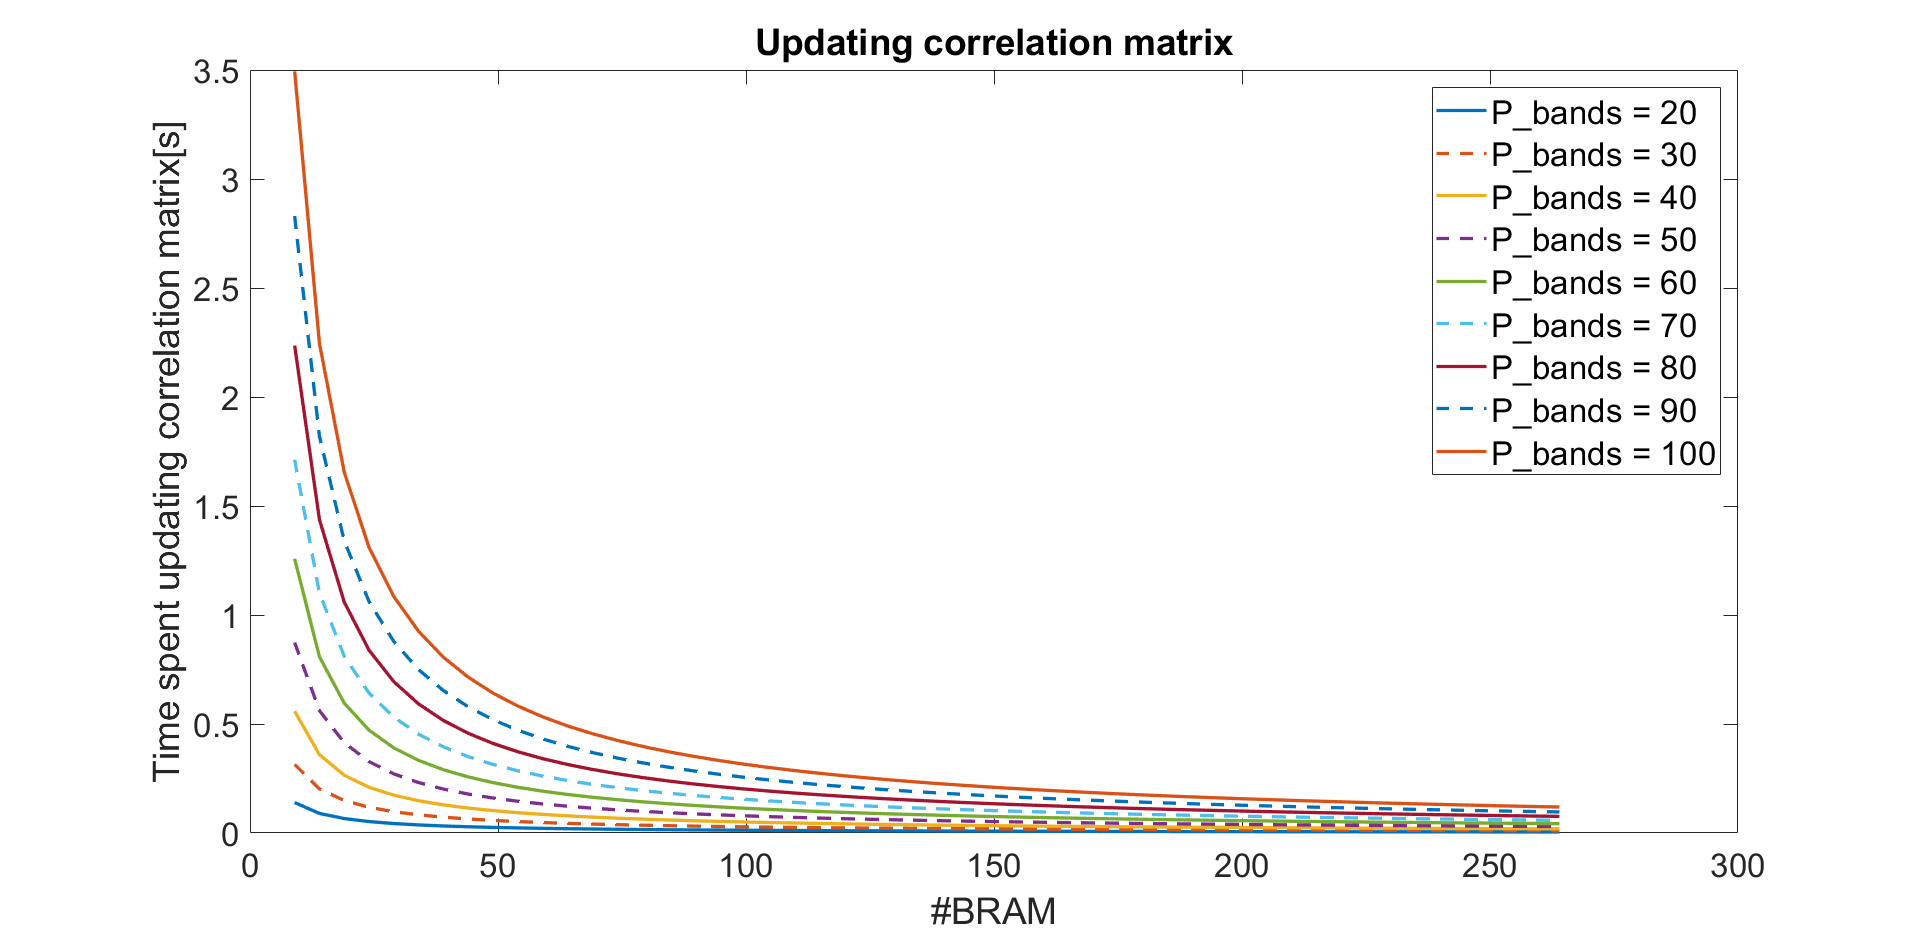
\includegraphics[scale=0.3]{images/time_spent_updating_correlation_matrix.png}}
  \caption{Estimated time spent updating $\Tilde{\textbf{R}}(\textbf{x}_k)$. } 
  \label{fig:update_time_correlation_BRAM}
\end{figure}

Two 18kbit SDPs are contained within one 36kbit BRAM block. \textbf{BRAM\_X\_EVEN} contains even  This is shown in Figure \ref{fig:BRAM_hierarchy}. The width of the addresses $WRADDR$ and $RADDR$ will be $log_2(\frac{P\_bands}{2})-1$.


\begin{figure}[H]
\centering

   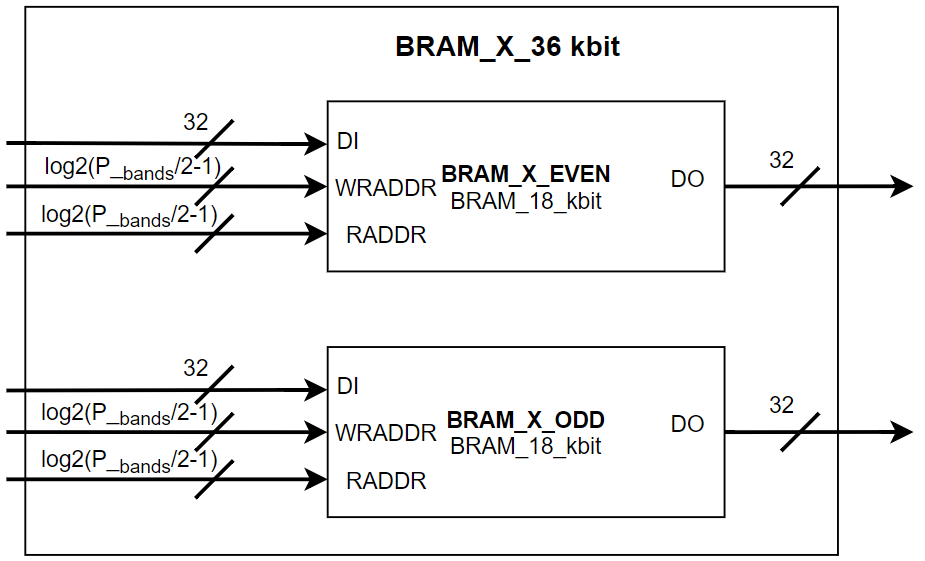
\includegraphics[scale=0.5]{images/BRAM_two_18_kbit.PNG}
  \caption{BRAM hierarchy, showing two 18kbit BRAM blocks contained within one 36kbit BRAM block. } 
  \label{fig:BRAM_hierarchy}
\end{figure}



\section{Proposed implementation}

The top level architecture of the ACAD Anomaly detector is shown in Figure \ref{fig:top_level_ACAD}. It consists of five blocks; \textbf{FSM ACAD}, \textbf{Shiftregister}, \textbf{ACAD correlation module}, \textbf{ACAD inverse module Gauss Jordan} and \textbf{dACAD module}.

\begin{figure}[H]
\refstepcounter{figure}
\begin{tabular}{c|c}

   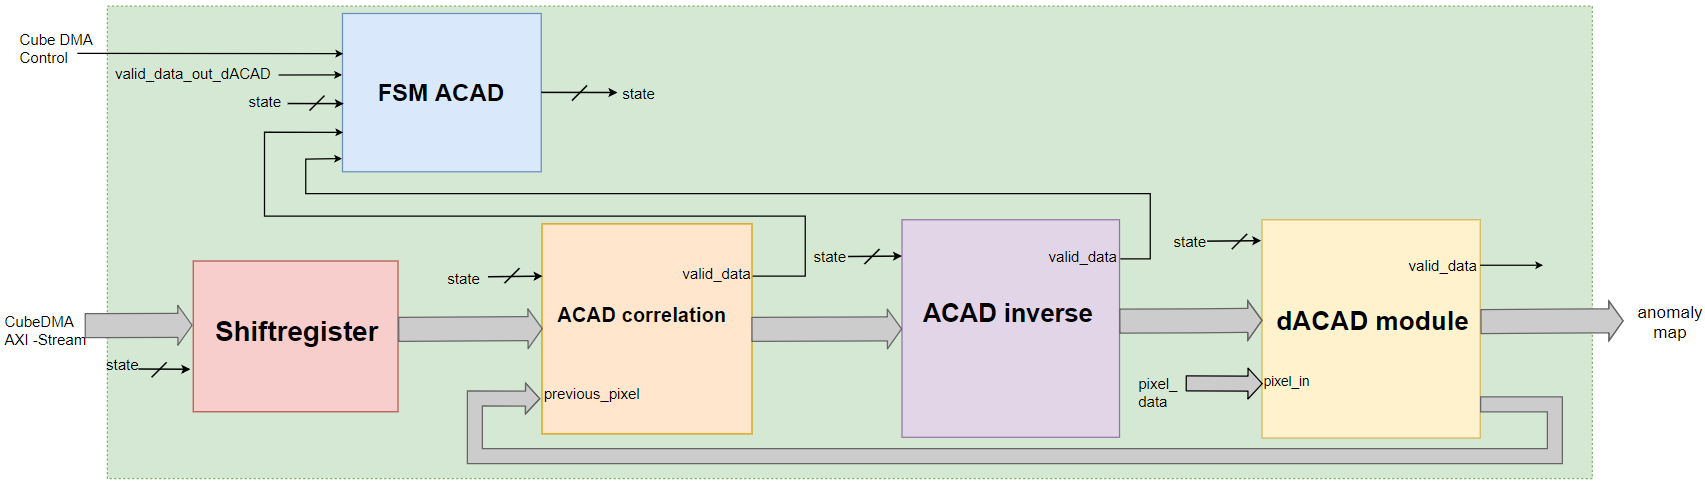
\includegraphics[scale=0.54, angle=90, origin=c]{images/acad_top_level.PNG}
   \rotatebox[origin=c]{90}{ Figure~\thefigure: Top level architecture of the ACAD anomaly detector.}
  %\caption{ \textbf{ROTATE}FSM controlling the architecture shown in Figure  } 
  \end{tabular}
  \label{fig:top_level_ACAD}
\end{figure}

The $\textbf{Shiftregister}$ is a $P\_bands$ $\times$ $Pixel\_data\_width$ $\times$ 2 AXI-LITE compatible shiftregister. It gets input pixel data from the CubeDMA used by the Smallsat project. 64 bit data is shifted in per clock cycle. For $Pixel\_data\_width$ of 16, this means 4 bands are shifted in per cycle. When a complete pixel is shifted in, it is sent to the $\textbf{ACAD correlation module}$, which computes the matrix $\Tilde{\textbf{R}}(\textbf{x}_k)$. $\Tilde{\textbf{R}}(\textbf{x}_k)$ is then outputted two rows at the time to the $\textbf{ACAD inverse}$ module, which computes $\Tilde{\textbf{R}^{-1}}(\textbf{x}_k)$.\\

Two rows of the inverse matrix is then sent to the $\textbf{dACAD module}$ per clock cycle. This block computes $\delta^{ACAD}$, as shown in Equation \ref{eq:ACAD_2}: 


\begin{equation}
    \delta^{ACAD}(\textbf{x}_k)= \textbf{x}_k^T\Tilde{\textbf{R}}^{-1}(\textbf{x}_k)\textbf{x}_k.
    \label{eq:ACAD_2}
\end{equation}

$u_k$ and $t_k$ is calculated to decide if the pixel is anomalous or not. When all pixels have been processed, the generated anomaly map is outputted, and the ACAD anomaly detection is finished.   
\\

The $\textbf{FSM\_ACAD}$ block controls the state of the ACAD anomaly detector. 


%\section{Memory considerations}
%%\label{sec:memory_management}
 %   As the ACAD anomaly detector is to be implemented on a Zynq Z-7030 or Z-7035 device, care must be taken when designing, with respect to logic and memory usage. As the hyperspectral image data inputted to the AD might have $P\_BANDS$=100, with 16-bit image data per spectral band, memory usage is an important consideration.   





\section{Shiftregister}
\textbf{THIS IS A SHIFTREGISTER OF FOUR BANDS(PIXELS) for pixel-datawidth of 16}


\section{ACAD correlation}
\label{sec:correlation_hw}
The \textbf{ACAD correlation module}, as shown in Figure \ref{fig:top_level_ACAD}, computes the ACAD correlation matrix $\Tilde{\textbf{R}}_{k x k}(\textbf{x}).
\\

As the SmallSat project is in the early phases, the value of $P\_bands$ for the data inputted to the AD from preprocessing steps are insecure. Another insecurity is the performance of the ACAD AD using PCA pre-processing, i.e. reducing the number of spectral bands in the AD. In addition, the ACAD AD requires storing of the inverse matrix, and the sum of anomaly detected. This is shown in figure X ( insert a figure showing the equation and what needs to be stored where). It is therefore not desirable to store the entire correlation matrix in flip flops, as there will be a need for storing other matrices, either in BRAM or DRAM, thereby inserting a bottleneck in the pipeline relative to the flip flop-updating step. Using BRAMs it is also possible to make a scalable solution for both small and large $p$. 
\\


As shown in Figure \ref{fig:update_time_correlation_BRAM} the time spent updating the correlation matrix can be reduced by increasing number of 36kbit BRAMs used to store the correlation matrix. By setting the  number of 36kbit BRAMs used to store the correlation matrix, $N\_BRAMS\_correlation$, equal to $P\_BANDS$ it is possible to store one column of the correlation matrix in each BRAM. This simplifies the control logic while achieving an acceptable trade off between speedup as a function of number of BRAMs used and resources used. Figure \ref{fig:data_flow_cube_dma_to_inverse} shows the data flow from the Cube DMA through the ACAD correlation module, with $N\_BRAM\_correlation$ =$P\_BANDS$. 
\\


\begin{figure}[H]
\centering
   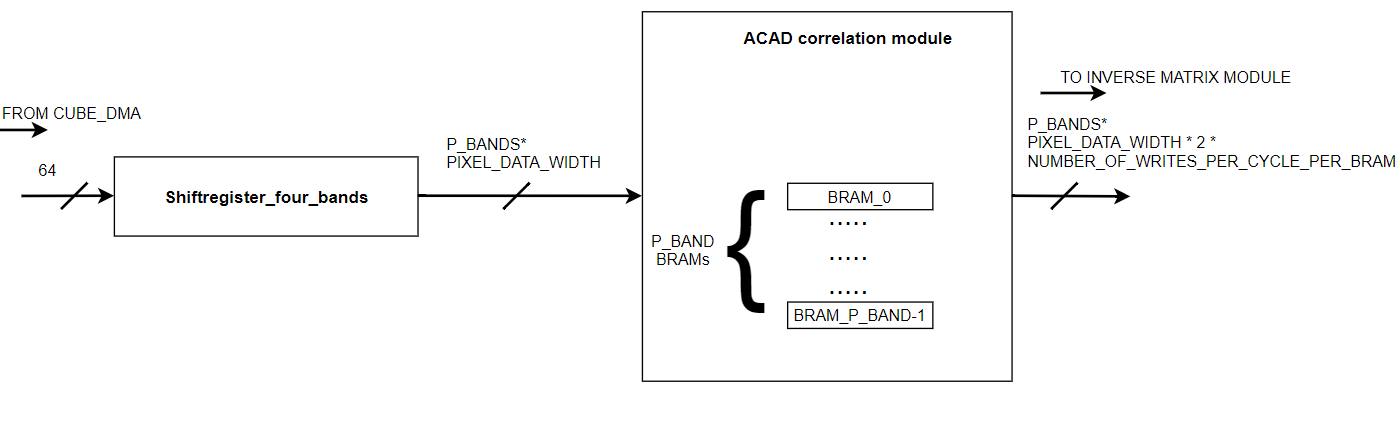
\includegraphics[scale=0.5]{images/data_flow_cube_dma_to_inverse_module.PNG}
  \caption{Data flow from Cube DMA via shiftregister to correlation module. Output on right hand side are input for inverse matrix computation module.  } 
  \label{fig:data_flow_cube_dma_to_inverse}
\end{figure}

Setting $N\_BRAMS\_correlation$ = $P\_BANDS$ allows to write to $P\_BANDS$ number of columns of the correlation matrix at the same time. As it is possible to write two 32 bit elements per cycle for each 36 kbit BRAM block, the total correlation matrix update time per pixel is $\frac{P\_BANDS}{2}$. 


The design is made for an even number of $P\_BANDS$. If odd number of spectral band is used, a band with zero values has to be inserted before inputting to the correlation module.\\

The design is made to be scalable with $P\_BANDS$, and will synthesize $P\_BANDS$ 36 kbit BRAMs and $P\_BANDS * 2$ DSP48E1(used for multiplication). By changing the value of the constant $P\_BANDS$ found in the $common\_types\_and\_functions$ package, the number of correlation sub-modules is changed. These sub-modules are shown in Figure \ref{fig:data_flow_correlation}. 
\begin{figure}[H]
\centering
   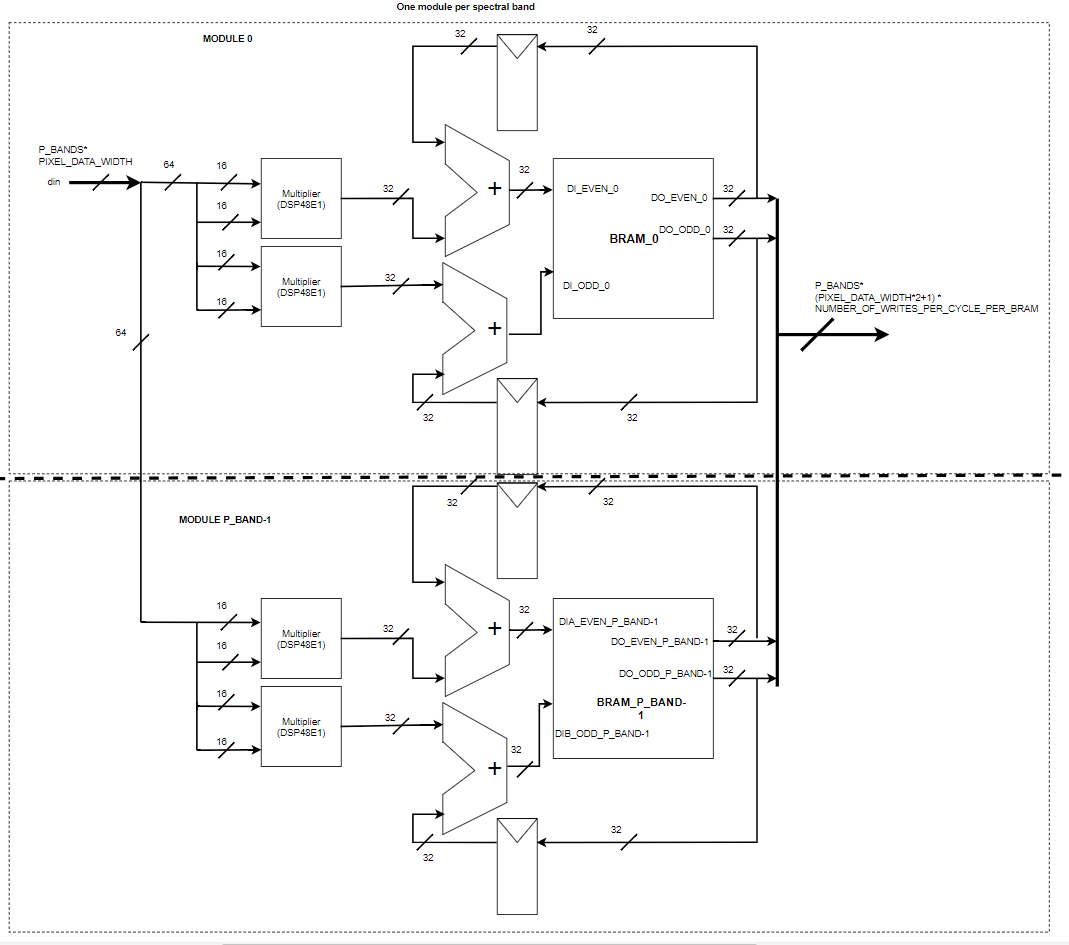
\includegraphics[scale=0.6]{images/correlation_data_path_with_adders.PNG}
  \caption{Data flow within the correlation module. The dotted lines marks one correlation sub-module. $P\_BANDS$ such modules are synthesized in the design. } 
  \label{fig:data_flow_correlation}
\end{figure}

The design was synthesized for $P\_BANDS$=10,20,30,40,50,60,70,80,90,100. Synthesis results show that the design scales as expected with respect to number of BRAM36E1 and DSP48E1 used. Figure \ref{fig:primitves_correlation}  shows the number of synthesized primitives  BRAM36E1 and DSP48E1. Figure \ref{fig:luts_and_regs_corr} shows number of synthesized SLICE REGISTERS and SLICE LUTS as a function of $P\_BANDS$.

\begin{figure}[H]

\hbox{\hspace*{-2cm}                                                           
   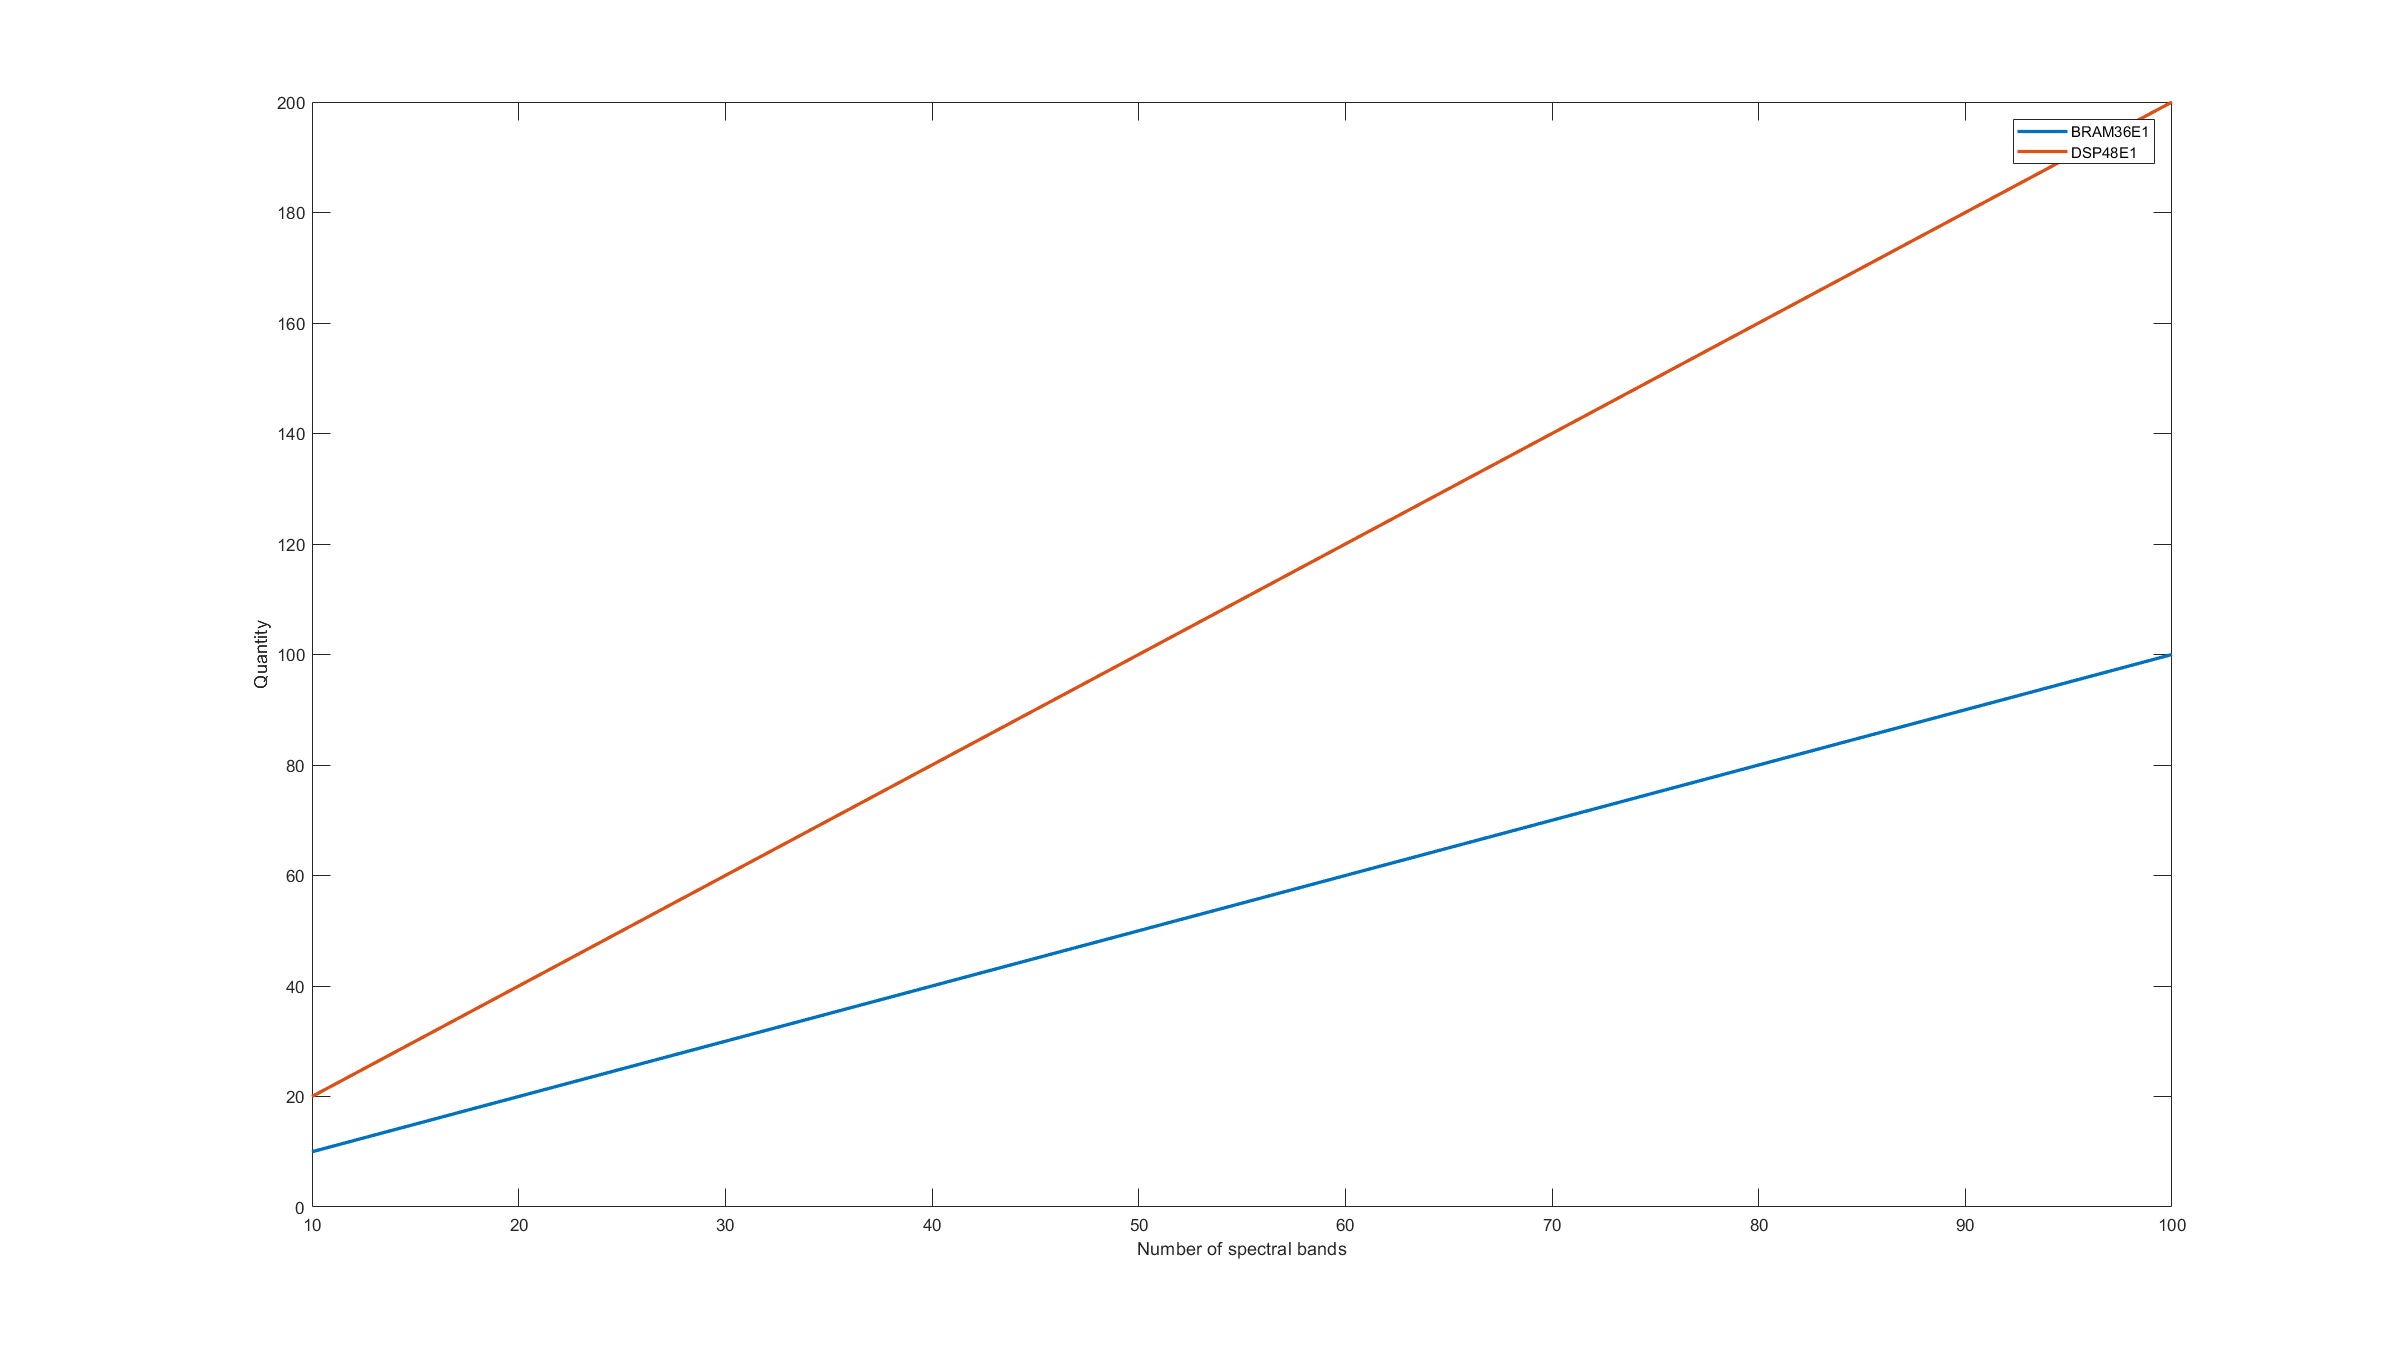
\includegraphics[scale=0.3]{images/number_of_BRAMS_and_DSP48.png}}
  \caption{Number of synthesized BRAM36E1 and DSP48E1 as a function of $P\_BANDS$. Results gathered from synthesis utilization report. } 
  \label{fig:primitves_correlation}
\end{figure}


\begin{figure}[H]

\hbox{\hspace*{-2cm}                                                           
   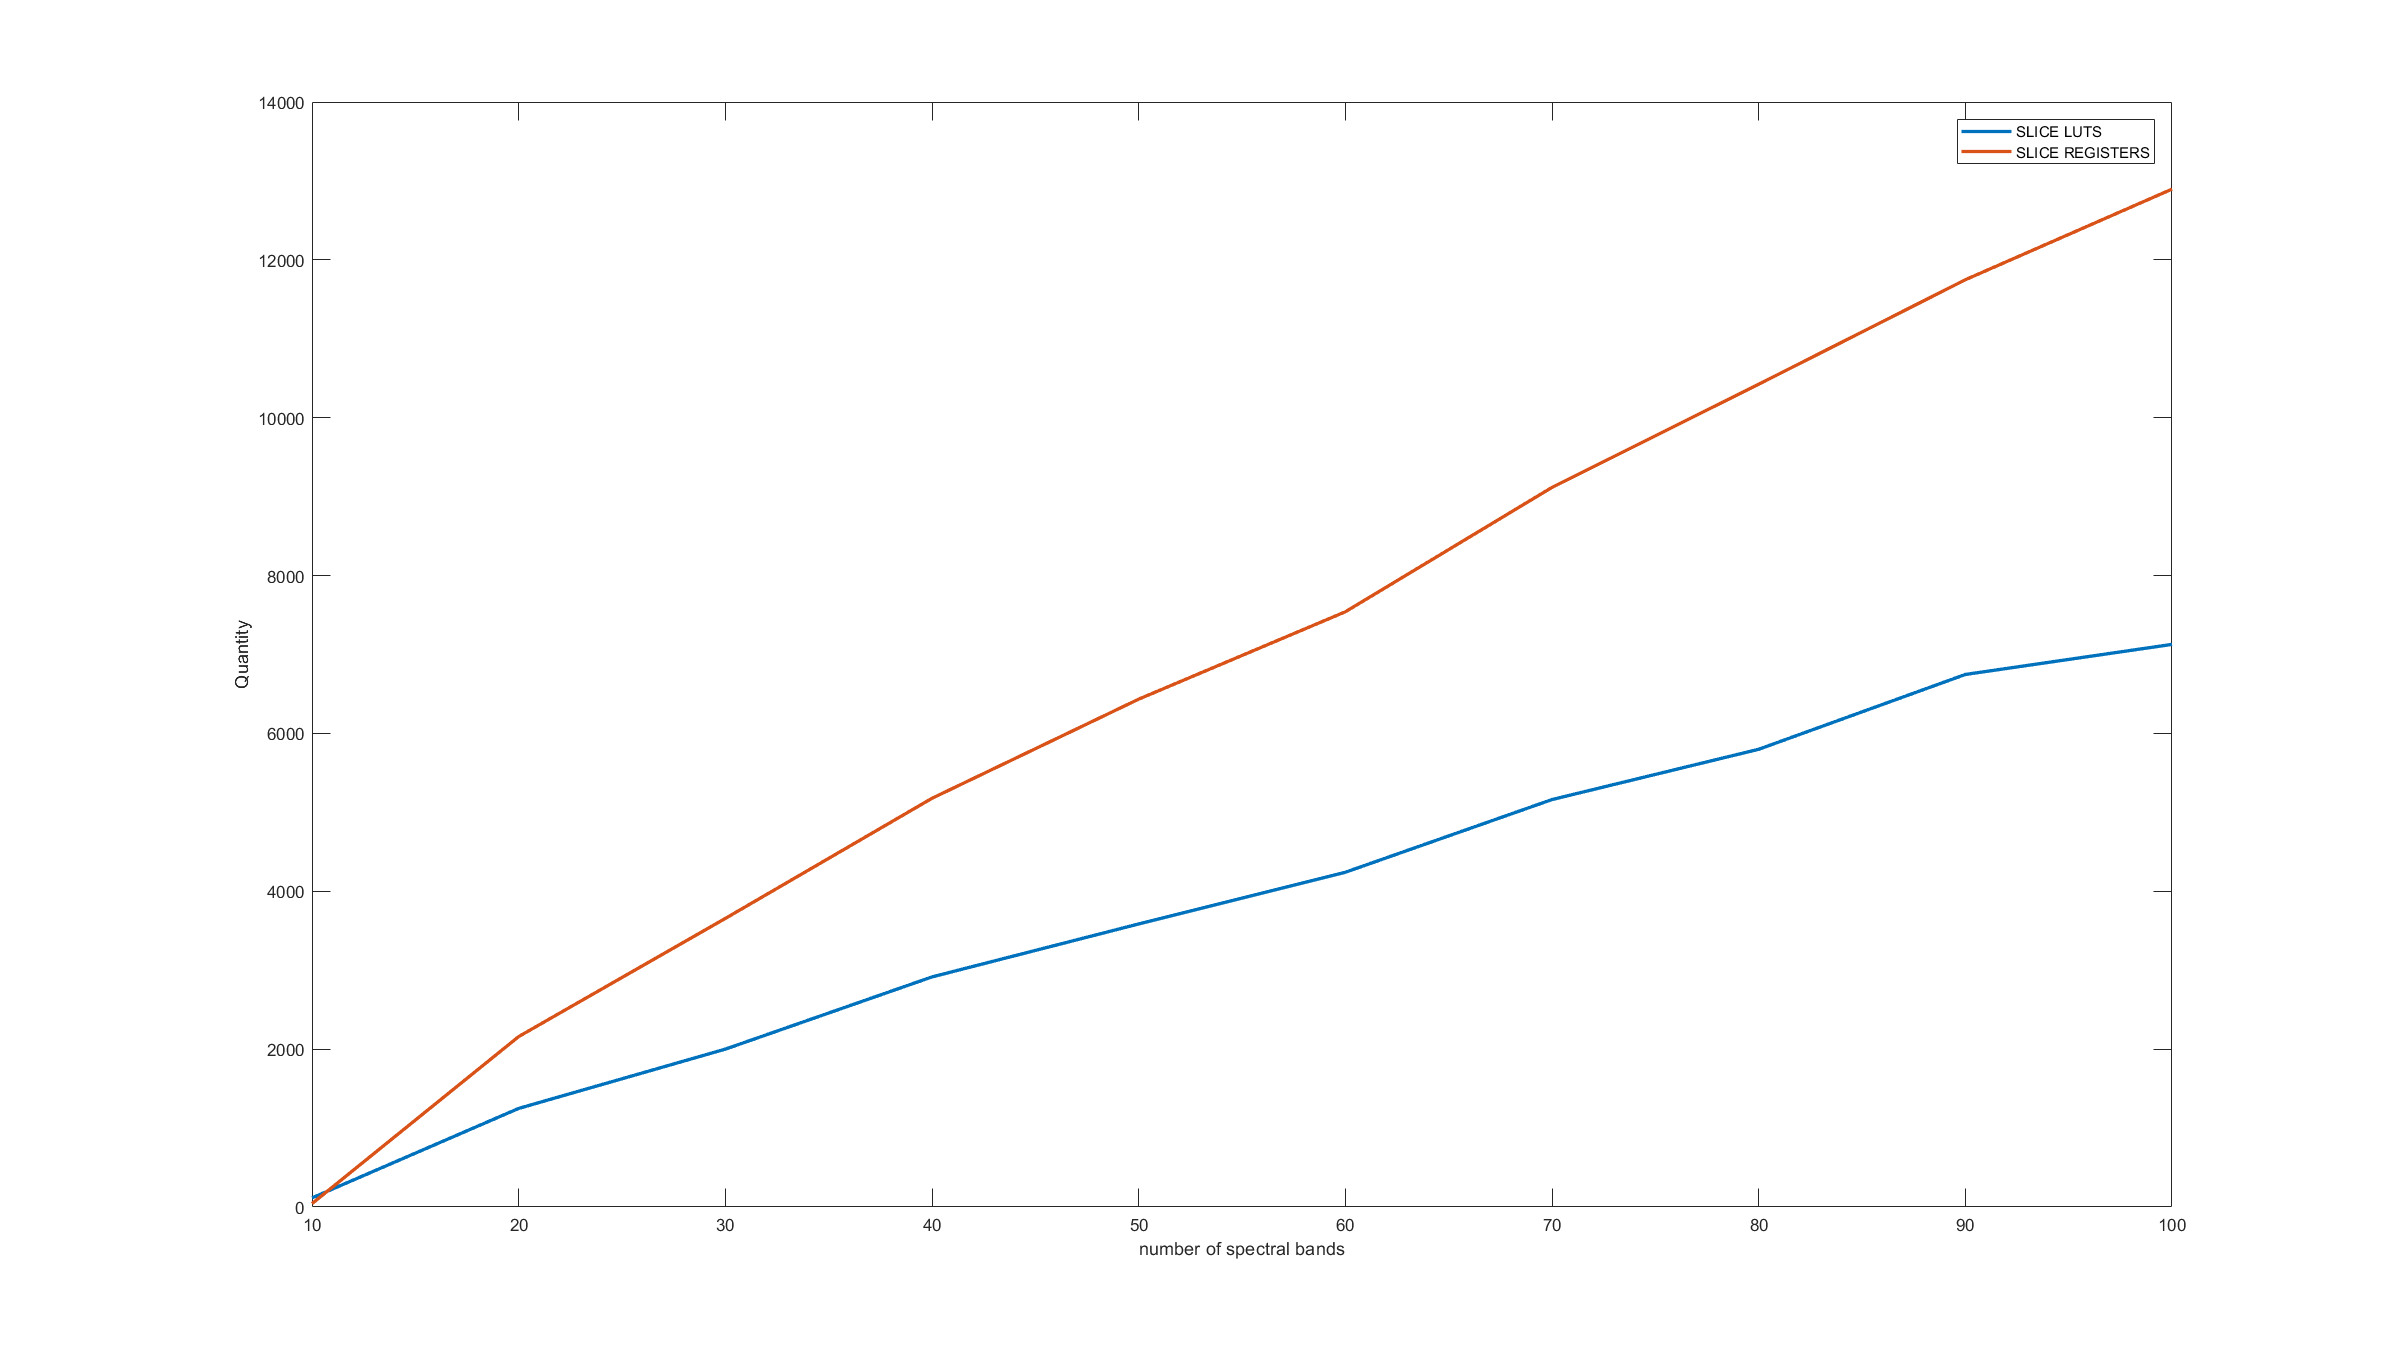
\includegraphics[scale=0.3]{images/correlation_luts_and_registers.png}}
  \caption{Number of synthesized SLICE REGISTERS and SLICE LUTS as a function of $P\_BANDS$. Results gathered from synthesis utilization report. } 
  \label{fig:luts_and_regs_corr}
\end{figure}


Pixel data inputted to the correlation module is inputted as a horizontal vector. For ACAD, the correlation matrix is presented in equation \ref{eq:caus_corr}. The correlation matrix is written to $N\_BRAM\_correlation$ in parallel, where the leftermost column(column zero) of the correlation matrix is written to BRAM\_0, column one to BRAM\_1,.. column P\_BANDS-1 to BRAM\_P\_BANDS-1. For each 36 kbit BRAM, two 18kbit BRAM blocks are accessed, one for even indexes of the column, and one for odd indexes of the column. This is also shown in figure \ref{fig:BRAM_hierarchy}. In Figure \ref{fig:BRAM_matrix} the addressing scheme for each 36kbit BRAM is presented, exemplified by BRAM\_0 and BRAM\_P\_BANDS-1. As shown in the figure, elements of column zero is stored in BRAM\_0, while elements of column P\_BANDS-1 is stored in BRAM\_P\_BANDS-1. Each 36 kbit BRAM consists of two 18 kbit blocks, storing even and odd row-index elements respectively. 

%the write sequence for each 36kbit BRAM is presented, exemplified by BRAM0. Here, the vertical vector element is din[PIXEL\_DATA\_WIDTH-1:0], shown by the blue line. The green lines shows data processed and BRAM written to during the first clock cycle. The red lines marks the second clock cycle and the orange lines marks the last clock cycle.  



\begin{figure}[H]
\centering
   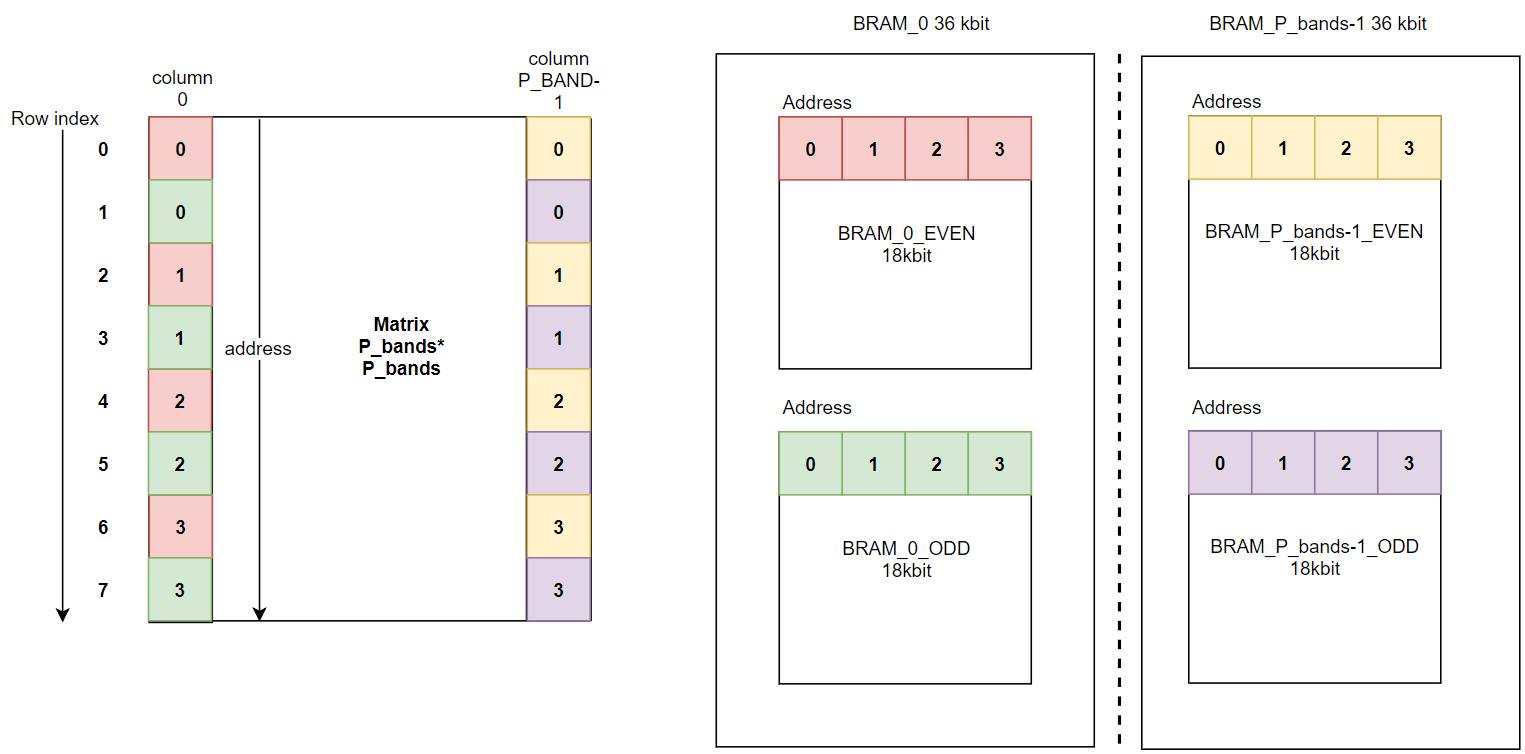
\includegraphics[scale=0.5]{images/bram_addressing_matrix.PNG}
  \caption{Storing matrix elements in different 36kbit BRAMs, storing one column of a matrix per BRAM. Each 36 kbit BRAM consists of two 18kbit BRAM blocks, one block storing even indexes of the matrix column, and one block storing odd indexes of the matrix column.    } 
  \label{fig:BRAM_matrix}
\end{figure}





\section{Inverse computation}
\label{sec:inverse_computation_hw}
Due to its low complexity, the Gauss-Jordan elimination was chosen to compute the inverse. A drawback with this algorithm is that it uses division. Division is an operation that is computationally intensive in hardware, and requires a large amount of logic to be implemented. An early implementation of the Gauss-Jordan elimination by the author included the use of the division operator "/". This is further described in Section \ref{sec:division_operator}.


%This approach utilized $P\_BANDS$ numbers of divisions, to ensure that one row of the inverse matrix could be computed in one clock cycle. The inner loop operation of forward and backward elimination in Figure \ref{fig:gauss_jordan_pseudocode} for this approach is shown in Figure .  A scaling problem became apparent, as this approach utilized too many LUTs as functions.  This is showed in the results, section \ref{sec:synthesis:luts_and_registers_inverse}. 
%Another approach was made, \textbf{INSERT figures here}..

An approach to implement division by adaptive shifting is described in Section \ref{sec:adaptive_shifting}. 

A third approach for computing division was made. This approach utilizes a large number of LUTs. It is further described in Section \ref{sec:LUT_division}.

%%\begin{figure}[H]
%%\centering
%%   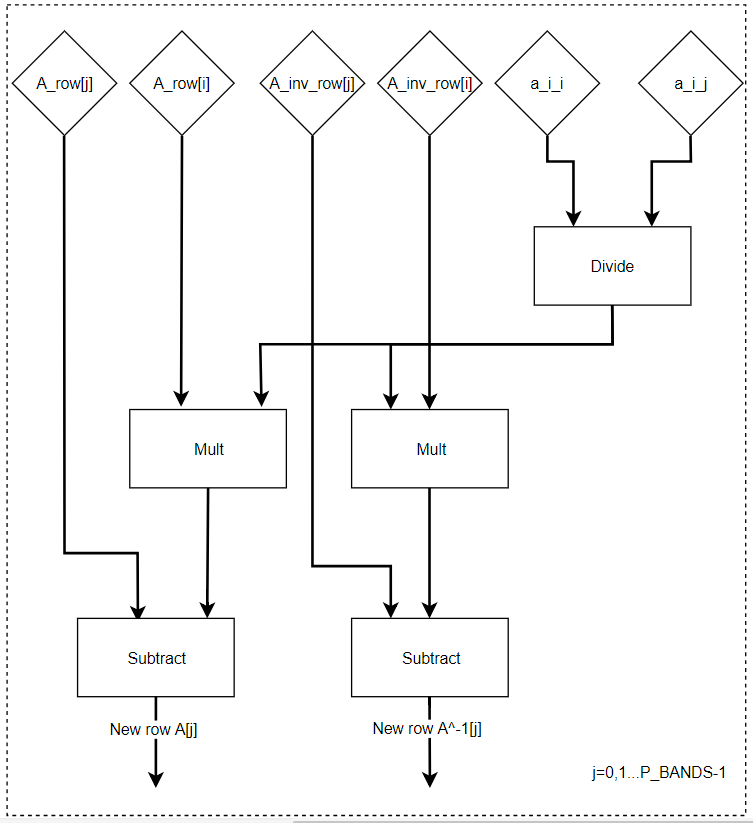
\includegraphics[scale=0.5]{images/inverse_approach_P_BANDS_divisions/inverse_core_old_approach.PNG}
%%  \caption{Architecture showing the first approach to implementing the forward and backward inner loop operation from Figure \ref{fig:gauss_jordan_pseudocode}. $P\_BANDS$ modules marked by the dotted border was synthesized.  } 
%%  \label{fig:inverse_P_BANDS_number_of_divisions}
%%\end{figure}


\subsection{Top level architecture}
The top level architecture of the inverse module can be seen in Figure \ref{fig:top_level_inverse}. This is an implementation of the Gauss-Jordan algorithm shown in Figure \ref{fig:gauss_jordan_pseudocode}. The \textbf{Forward elimination} block correspond to operations marked by the black square in Figure \ref{fig:gauss_jordan_pseudocode}, while \textbf{Backward elimination} and \textbf{Last division} blocks correspond to the operations marked by the red and green squares in Figure \ref{fig:gauss_jordan_pseudocode} respectively, with an exception to the operations shown in Figure \ref{fig:elimination_inner_core_pseudocode}.These operations are part of both the forward elimination and backward elimination blocks in the Gauss-Jordan inverse. They are therefore put in an external process, called \textbf{Elimination core}. 
\\

\textbf{A} and \textbf{A\_inv} are two BRAM36 arrays of size $P\_BANDS$, in which $\textbf{A}$ and $\textbf{A}^{-1}$ are stored, respectively. 

\begin{figure}[H]
\centering
   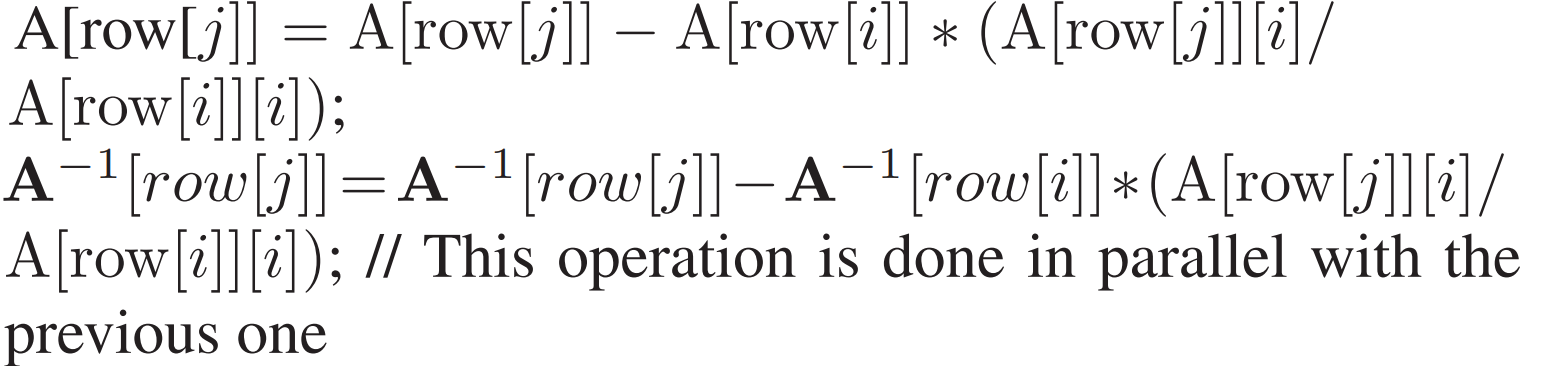
\includegraphics[scale=0.3]{images/inverse_hw/elimination_inner_core_pseudocode.PNG}
  \caption{The operations computed by the \textbf{Elimination core}, utilized by both the \textbf{Forward elimination} and the \textbf{Backward elimination} block.  } 
  \label{fig:elimination_inner_core_pseudocode}
\end{figure}


\begin{figure}[H]
\refstepcounter{figure}
\begin{tabular}{c|c}

   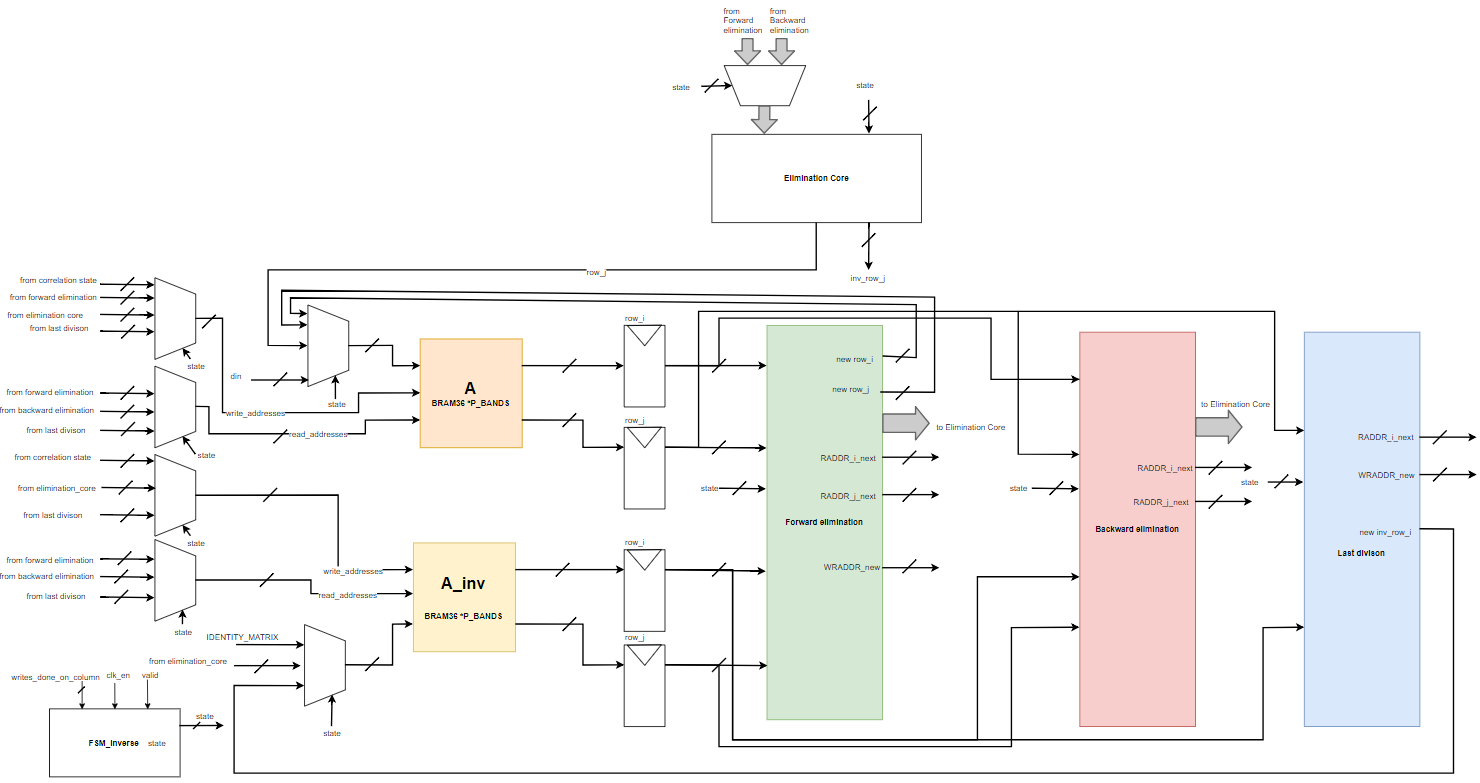
\includegraphics[scale=0.7, angle=90, origin=c]{images/inverse_hw/top_level_architecture_inverse.PNG}
   \rotatebox[origin=c]{90}{ Figure~\thefigure: Top level architecture of the inverse module.}
  %\caption{ \textbf{ROTATE}FSM controlling the architecture shown in Figure  } 
  \end{tabular}
  \label{fig:top_level_inverse}
\end{figure}



\subsection{Top level inverse FSM}
The state machine for the inverse module shown in Figure \ref{fig:top_level_inverse} is shown in Figure \ref{fig:fsm_inverse_matrix}. Its possible states are explained in Table \ref{tab:fsm_inverse}.

\begin{table}[H]
\centering
 \resizebox{1\textwidth}{!}
{\begin{tabular}{l|l}
State                                                                                    & Description                                                                                   \\
\hline
\textbf{Unknown state}                                                                   & An unknown state. The behaviour of the inverse module is unknown. The FSM should transition to state Idle.                                    \\
\textbf{Idle}                                                                            & The inverse module is not performing any operations.                                          \\
\textbf{\begin{tabular}[c]{@{}l@{}}Store\_correlation\_matrix\_\\ in\_BRAM\end{tabular}} & Writing data from correlation module to BRAMs. Two rows written to BRAMs per clock cycle.     \\
\textbf{Forward\_elimination}                                                            & Computing the forward elimination of the Gauss-Jordan elimination as shown in Figure \ref{fig:gauss_jordan_pseudocode}.        \\
\textbf{Backward\_elimination}                                                           & Computing the backward elimination of the Gauss-Jordan elimination as shown in Figure \ref{fig:gauss_jordan_pseudocode}.       \\
\textbf{Last\_division}                                                                  & Computing the last division of the Gauss-Jordan elimination as shown in Figure \ref{fig:gauss_jordan_pseudocode}.              \\
\textbf{Output\_inverse\_matrix}                                                         & Outputting the finished inverse matrix for the pixel. Two rows are outputted per clock cycle.
\end{tabular}}
\caption{States of the inverse FSM}
\label{tab:fsm_inverse}

\end{table}

\begin{figure}[H]
\centering
   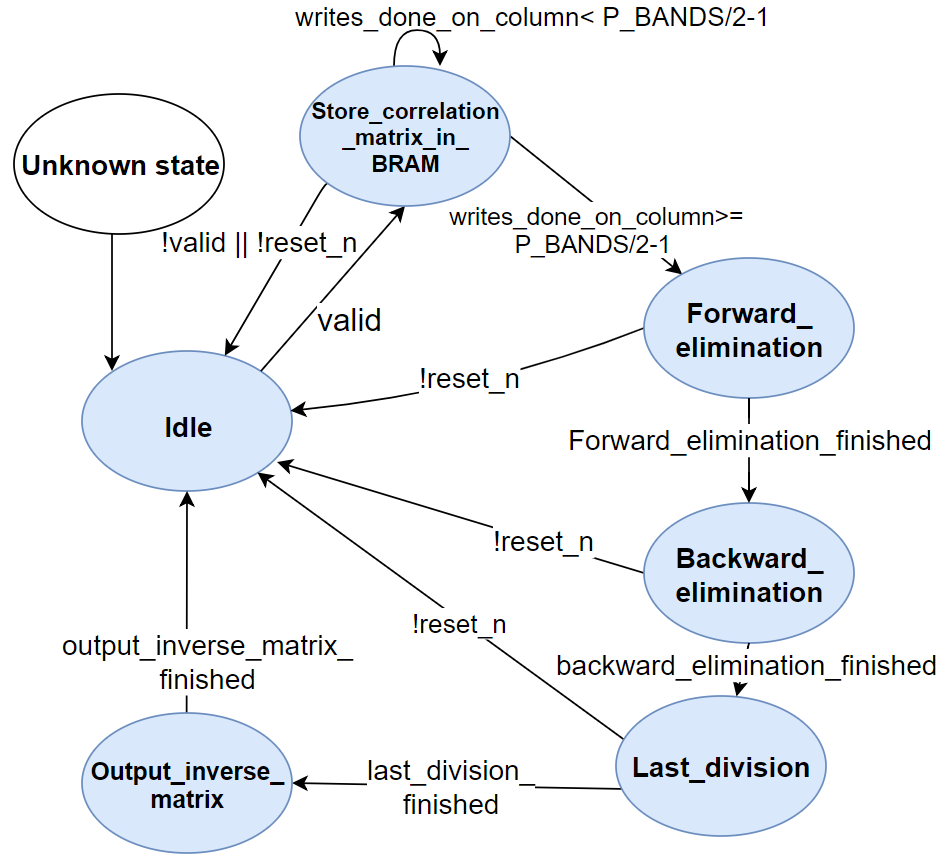
\includegraphics[scale=0.5]{images/inverse_hw/fsm_inverse_matrix.PNG}
  \caption{FSM controlling the architecture shown in Figure \ref{fig:top_level_inverse}.  } 
  \label{fig:fsm_inverse_matrix}
\end{figure}

The inverse module is controlled by the FSM shown in Figure \ref{fig:fsm_inverse_matrix}. 

\subsection{Forward elimination}
Forward elimination is defined as the operations trailing the   of the Gauss-Jordan elimination shown in Figure \ref{fig:gauss_jordan_pseudocode}.


\begin{table}[H]
\centering
 \resizebox{1\textwidth}{!}
{\begin{tabular}{l|l}
State                                                                                    & Description                                                                                   \\
\hline
\textbf{Unknown state}                                                                   & An unknown state. The behaviour of the inverse module is unknown. The FSM should transition to state Idle.                                    \\
\textbf{Idle}                                                                            & The forward elimination module is not performing any operations.                                          \\
\textbf{Check\_diagonal\_element\_is\_zero} & Checking if element row\_i[index\_i]= 0 as done in Gauss-Jordan elimination shown in Figure \ref{fig:gauss_jordan_pseudocode}.     \\
\textbf{Swap\_rows}                                                            & Swapping row\_i and row\_j of the matrix A as described in Figure \ref{fig:gauss_jordan_pseudocode}.        \\
\textbf{Even\_j\_write}                                                           & Updating an even indexed row of the matrix A and $A^{-1}$(described in Figure \ref{fig:gauss_jordan_pseudocode}).       \\
\textbf{Odd\_j\_write}                                                                  & Updating an odd indexed row of the matrix A and $A^{-1}$(described in Figure \ref{fig:gauss_jordan_pseudocode}).   
\end{tabular}}
\caption{States of the forward elimination FSM}
\label{tab:fsm_forward_elimination}

\end{table}


\begin{figure}[H]
\centering
   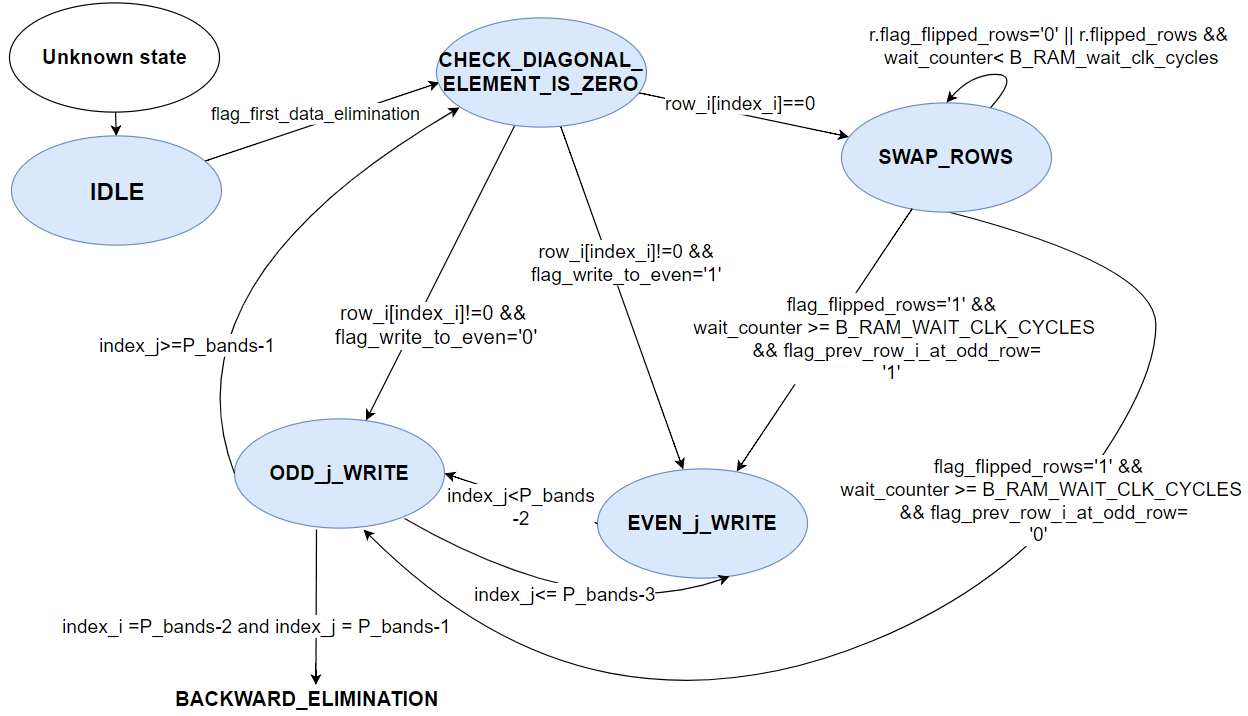
\includegraphics[scale=0.4]{images/inverse_hw/fsm_forward_elimination.png}
  \caption{FSM controlling the forward elimination state shown in Figure \ref{fig:fsm_inverse_matrix}.  } 
  \label{fig:fsm_forward_elimination}
\end{figure}


\subsection{Backward elimination}

\begin{table}[H]
\centering
 \resizebox{1\textwidth}{!}
{\begin{tabular}{l|l}
State                                                                                    & Description                                                                                   \\
\hline
\textbf{Unknown state}                                                                   & An unknown state. The behaviour of the inverse module is unknown. The FSM should transition to state Idle.                                    \\
\textbf{Idle}                                                                            & The forward elimination module is not performing any operations.                                          \\
\textbf{First\_elimination} & Checking if element row\_i[index\_i]= 0 as done in Gauss-Jordan elimination shown in Figure \ref{fig:gauss_jordan_pseudocode}.     \\
\textbf{Odd\_i\_start}                                                            & Starting at a new iteration of the outermost loop of the backward elimination loop in the Gauss-Jordan elimination shown in  \ref{fig:gauss_jordan_pseudocode}. 
\\
&
Starting at an odd row-index of the matrix. Computing A[row\_j] and $A^{-1}$[row\_j], which is at an even index. Updating matrices.       \\

\textbf{Even\_i\_start}                                                            & Starting at a new iteration of the outermost loop of the backward elimination loop in the Gauss-Jordan elimination shown in  \ref{fig:gauss_jordan_pseudocode}.
\\&
Starting at an even row-index of the matrix. Computing A[row\_j] and $A^{-1}$[row\_j], which is at an odd index. Updating matrix.        \\

\textbf{Even\_j\_write}                                                           & Updating an even indexed row of the matrix A and $A^{-1}$(described in Figure \ref{fig:gauss_jordan_pseudocode}).       \\
\textbf{Odd\_j\_write}                                                                  & Updating an odd indexed row of the matrix A and $A^{-1}$(described in Figure \ref{fig:gauss_jordan_pseudocode}).   
\end{tabular}}
\caption{States of the forward elimination FSM}
\label{tab:fsm_forward_elimination}

\end{table}

\begin{figure}[H]
\centering
   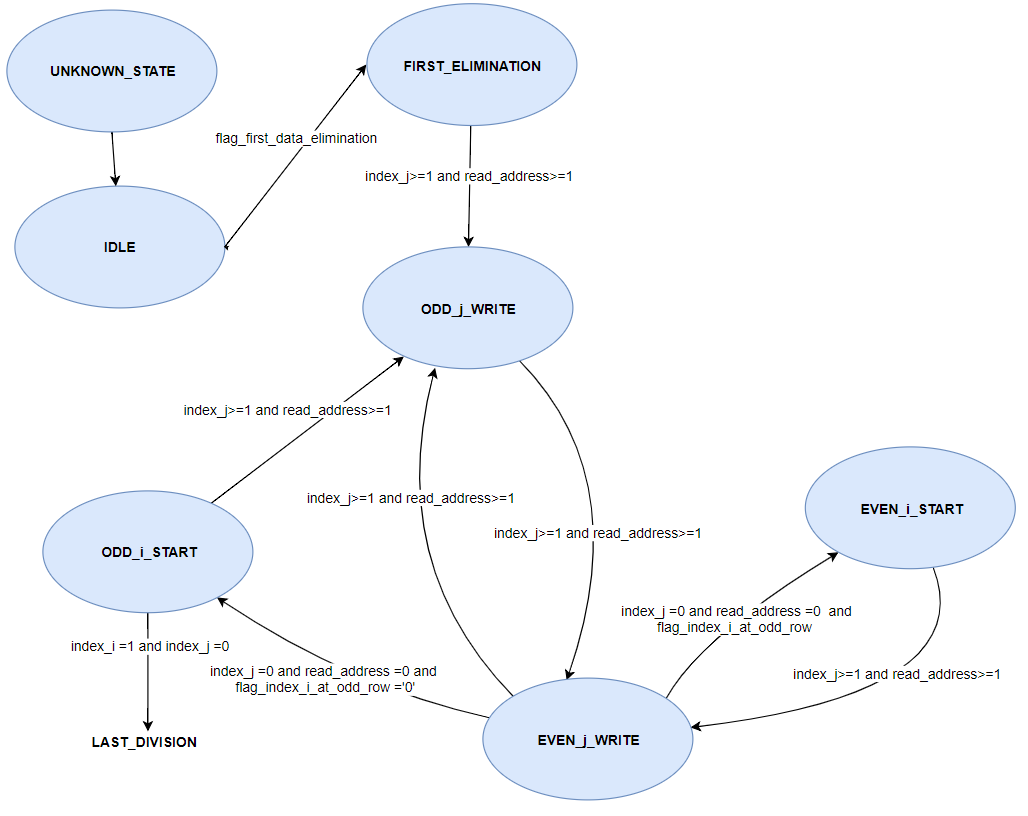
\includegraphics[scale=0.5]{images/inverse_hw/fsm_backward_elimination.PNG}
  \caption{FSM controlling the backward elimination state shown in Figure \ref{fig:fsm_inverse_matrix}.  } 
  \label{fig:fsm_backward_elimination}
\end{figure}

\subsection{Last division}

\begin{table}[H]
\centering
 \resizebox{1\textwidth}{!}
{\begin{tabular}{l|l}
State                                                                                    & Description                                                                                   \\
\hline
\textbf{Unknown state}                                                                   & An unknown state. The behaviour of the inverse module is unknown. The FSM should transition to state Idle.                                    \\
\textbf{Idle}                                                                            & The forward elimination module is not performing any operations.                                          \\


\textbf{Even\_i\_write}                                                           & Updating an even indexed row of the matrix $A^{-1}$(described in Figure \ref{fig:gauss_jordan_pseudocode}).       \\
\textbf{Odd\_i\_write}                                                                  & Updating an odd indexed row of the matrix $A^{-1}$(described in Figure \ref{fig:gauss_jordan_pseudocode}).   
\end{tabular}}
\caption{States of the last division FSM}
\label{tab:fsm_last_division}

\end{table}


\begin{figure}[H]
\centering
   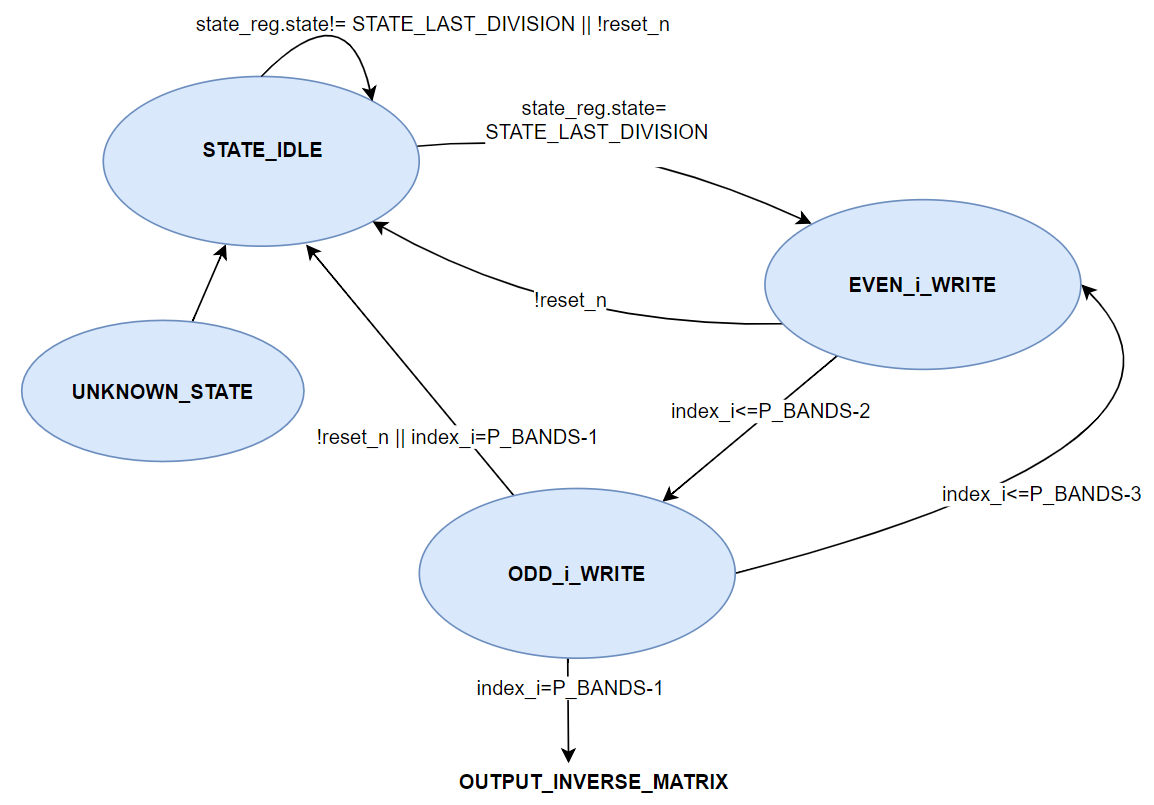
\includegraphics[scale=0.5]{images/inverse_hw/fsm_last_division.PNG}
  \caption{FSM controlling the last\_division state shown in Figure \ref{fig:fsm_inverse_matrix}.  } 
  \label{fig:fsm_last_division}
\end{figure}

\subsection{Memory hierarchy}
The Gauss Jordan inverse requires two matrices to be stored in memory, the matrix $\textbf{A}$ and $\textbf{A}^{-1}$ as shown in Figure \ref{fig:gauss_jordan_pseudocode}. Both of these matrices will be of the same size as the correlation matrix, described in section \ref{sec:mem_management_correlation_matrix}. It is therefore not desirable to store these matrices in registers, but rather in BRAM. By having the same memory structure as described in section \ref{sec:mem_management_correlation_matrix}, using $P\_BANDS$ BRAM 36kbit blocks for each of the matrices, this will enable two rows of each matrix to be written and read per clock cycle. 

\subsection{Inverse pipeline stages}
The inverse module is pipelined into four stages in order to achieve high throughput. The pipeline can be seen in Figure \ref{fig:pipeline_inverse_part_1}, \ref{fig:pipeline_inverse_part_2} and \ref{fig:pipeline_inverse_part_3}.

\begin{figure}[H]
\centering
   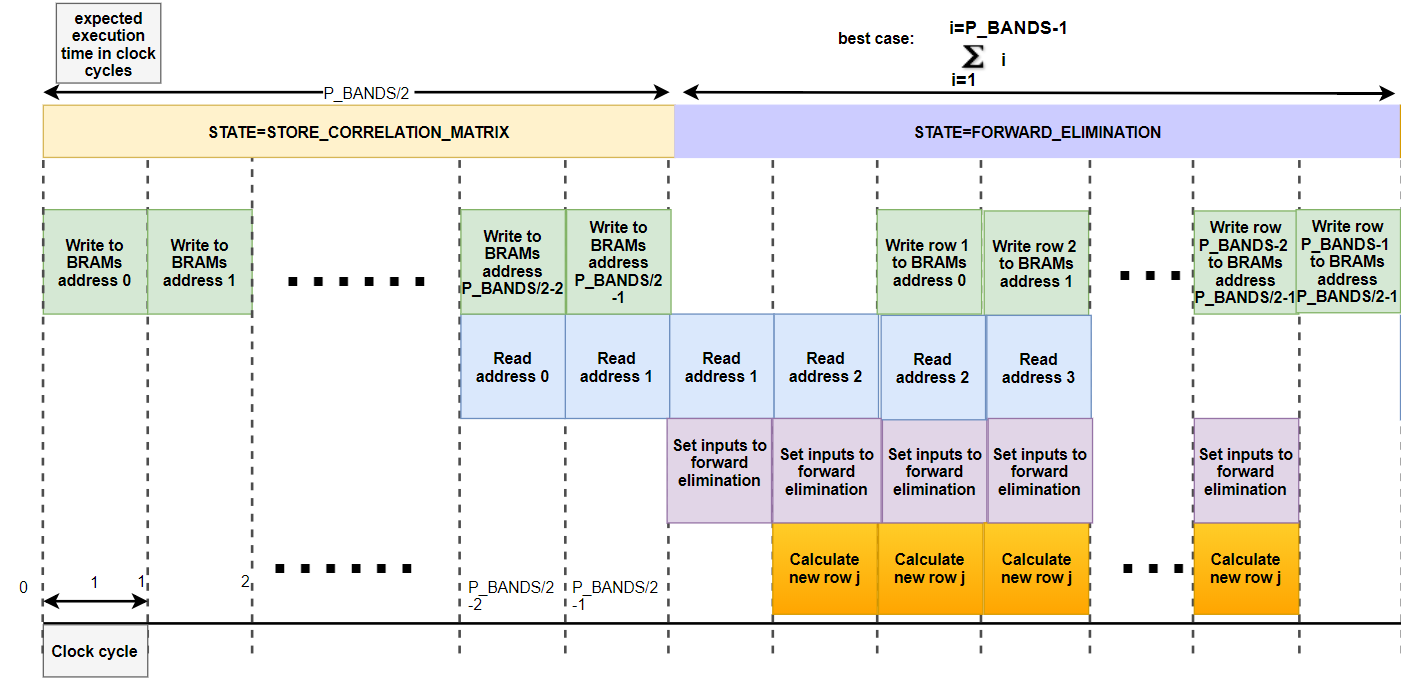
\includegraphics[scale=0.5]{images/estimation_execution_time/pipeline_inverse_matrix_part_1.PNG}
  \caption{Showing pipeline operations in the Store\_correlation\_matrix and Forward\_elimination states.  } 
  \label{fig:pipeline_inverse_part_1}
\end{figure}

\begin{figure}[H]
\centering
   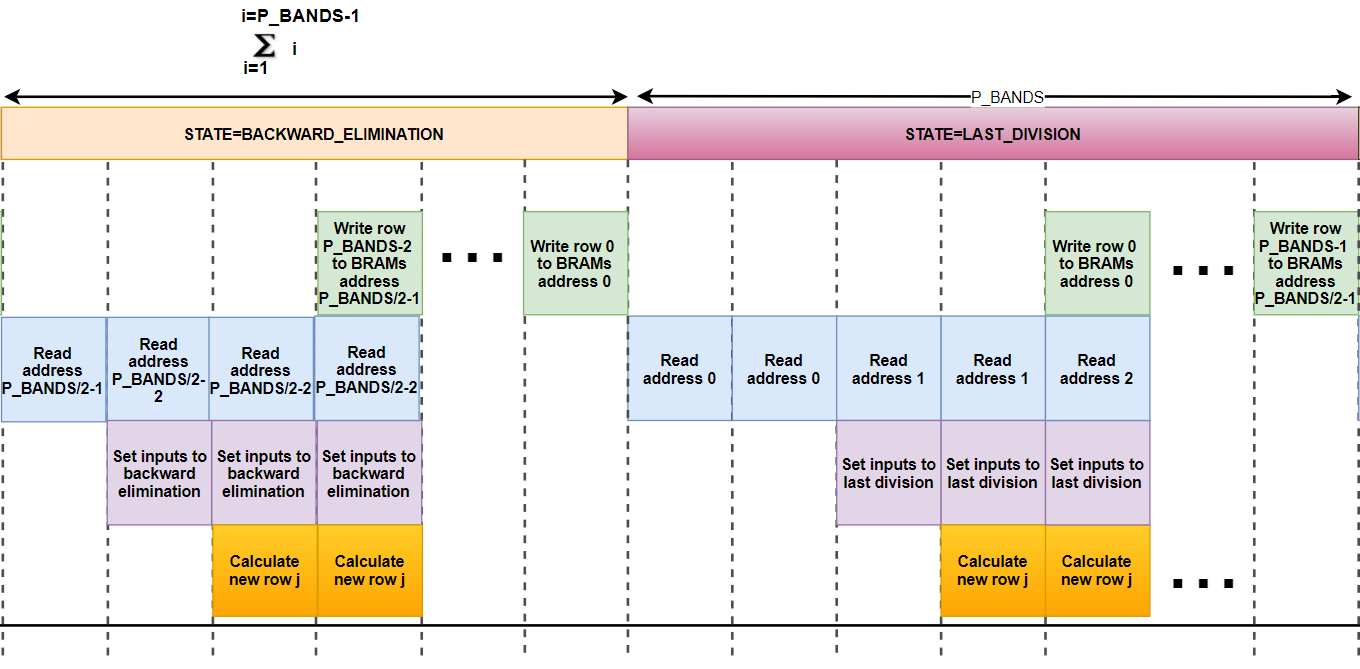
\includegraphics[scale=0.5]{images/estimation_execution_time/pipeline_inverse_matrix_part_2.PNG}
  \caption{Showing pipeline operations in the Forward\_elimination and Last\_division states.  } 
  \label{fig:pipeline_inverse_part_2}
\end{figure}

\begin{figure}[H]
\centering
   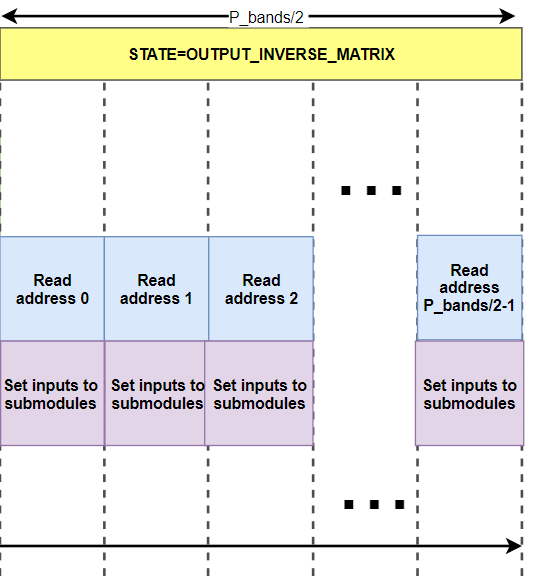
\includegraphics[scale=0.5]{images/estimation_execution_time/pipeline_inverse_matrix_part_3.PNG}
  \caption{Showing pipeline operations in the $Output\_inverse\_matrix$ state.  } 
  \label{fig:pipeline_inverse_part_3}
\end{figure}



\subsection{Execution time expectations}
Using $P\_BANDS$ BRAMs enables to read and write a maximum of two rows of each of the matrices $\textbf{A}$ and $\textbf{A}^{-1}$ per clock cycle.  Assuming that each of the row-operations in the Gauss-Jordan elimination can be calculated within one clock cycle, it is possible to do an estimation of the expected execution time in clock cycles for the inverse computation per pixel. \\

Expected execution time for the different states is shown in Figure \ref{fig:pipeline_inverse_part_1}, \ref{fig:pipeline_inverse_part_2} and \ref{fig:pipeline_inverse_part_3}. For state $Forward\_elimination$, the execution time will be greater if it is necessary to swap rows, shown by the state $SWAP\_ROWS$ in Figure \ref{fig:fsm_forward_elimination}. The worst case execution time of $Forward\_elimination$ is assumed to be when the first element of the matrix $\textbf{A}$ has a zero element at row(i,i) and all other rows,except the last row, has a zero element at row(j,j). \\

A worst case and a best case execution time, $inv\_worst\_case$ and $inv\_best\_case$, for the computation of the inverse per pixel is then estimated. The estimations are shown in Equation \ref{eq:inv_worst_case} and \ref{eq:inv_best_case}.$N\_STATES\_INV$ is the number of valid states in the inverse top level module, shown in Figure \ref{fig:fsm_inverse_matrix}. $worst\_case\_ex\_state$ is the set of expected worst case execution times for the states.  $best\_case\_ex\_state$ is the set of expected best case execution times for the states. 

\begin{equation}
\begin{split}
inv\_worst\_case & = \sum_{i=0}^{N\_STATES\_INV}worst\_case\_ex\_state(i) \\
& =\underbrace{\frac{P\_BANDS}{2} }_\text{STORE\_CORRELATION\_MATRIX}  + \overbrace{\sum_{i=0}^{P\_BANDS-1}i + P\_BANDS}^\text{STATE\_FORWARD\_ELIMINATION} \\
& + \underbrace{\sum_{i=0}^{P\_BANDS-1}i}_\text{STATE\_BACKWARD\_ELIMINATION}  
 +
\overbrace{P\_BANDS}^\text{LAST\_DIVISION} + \underbrace{P\_BANDS/2}_\text{OUTPUT\_INVERSE\_MATRIX}\\
& = 3P\_BANDS + 2\sum_{i=0}^{P\_BANDS-1}i
\end{split}
\label{eq:inv_worst_case}
\end{equation}


\begin{equation}
\begin{split}
inv\_best\_case & = \sum_{i=0}^{N\_STATES\_INV}best\_case\_ex\_state(i) \\
& = \underbrace{\frac{P\_BANDS}{2} }_\text{STORE\_CORRELATION\_MATRIX}  + \overbrace{\sum_{i=0}^{P\_BANDS-1}i }^\text{STATE\_FORWARD\_ELIMINATION} \\
& + \underbrace{\sum_{i=0}^{P\_BANDS-1}i}_\text{STATE\_BACKWARD\_ELIMINATION}  
 +
\overbrace{P\_BANDS}^\text{LAST\_DIVISION} + \underbrace{P\_BANDS/2}_\text{OUTPUT\_INVERSE\_MATRIX}\\
& = 2P\_BANDS + 2\sum_{i=0}^{P\_BANDS-1}i
\end{split}
\label{eq:inv_best_case}
\end{equation}

Figure \ref{fig:estimated_time_inverse} shows the estimated execution time in seconds for computing the inverse for all pixels in the hyperspectral image, for an image size of 1088x576. 

\begin{figure}[H]
\hbox{\hspace*{-3cm}                                                           

   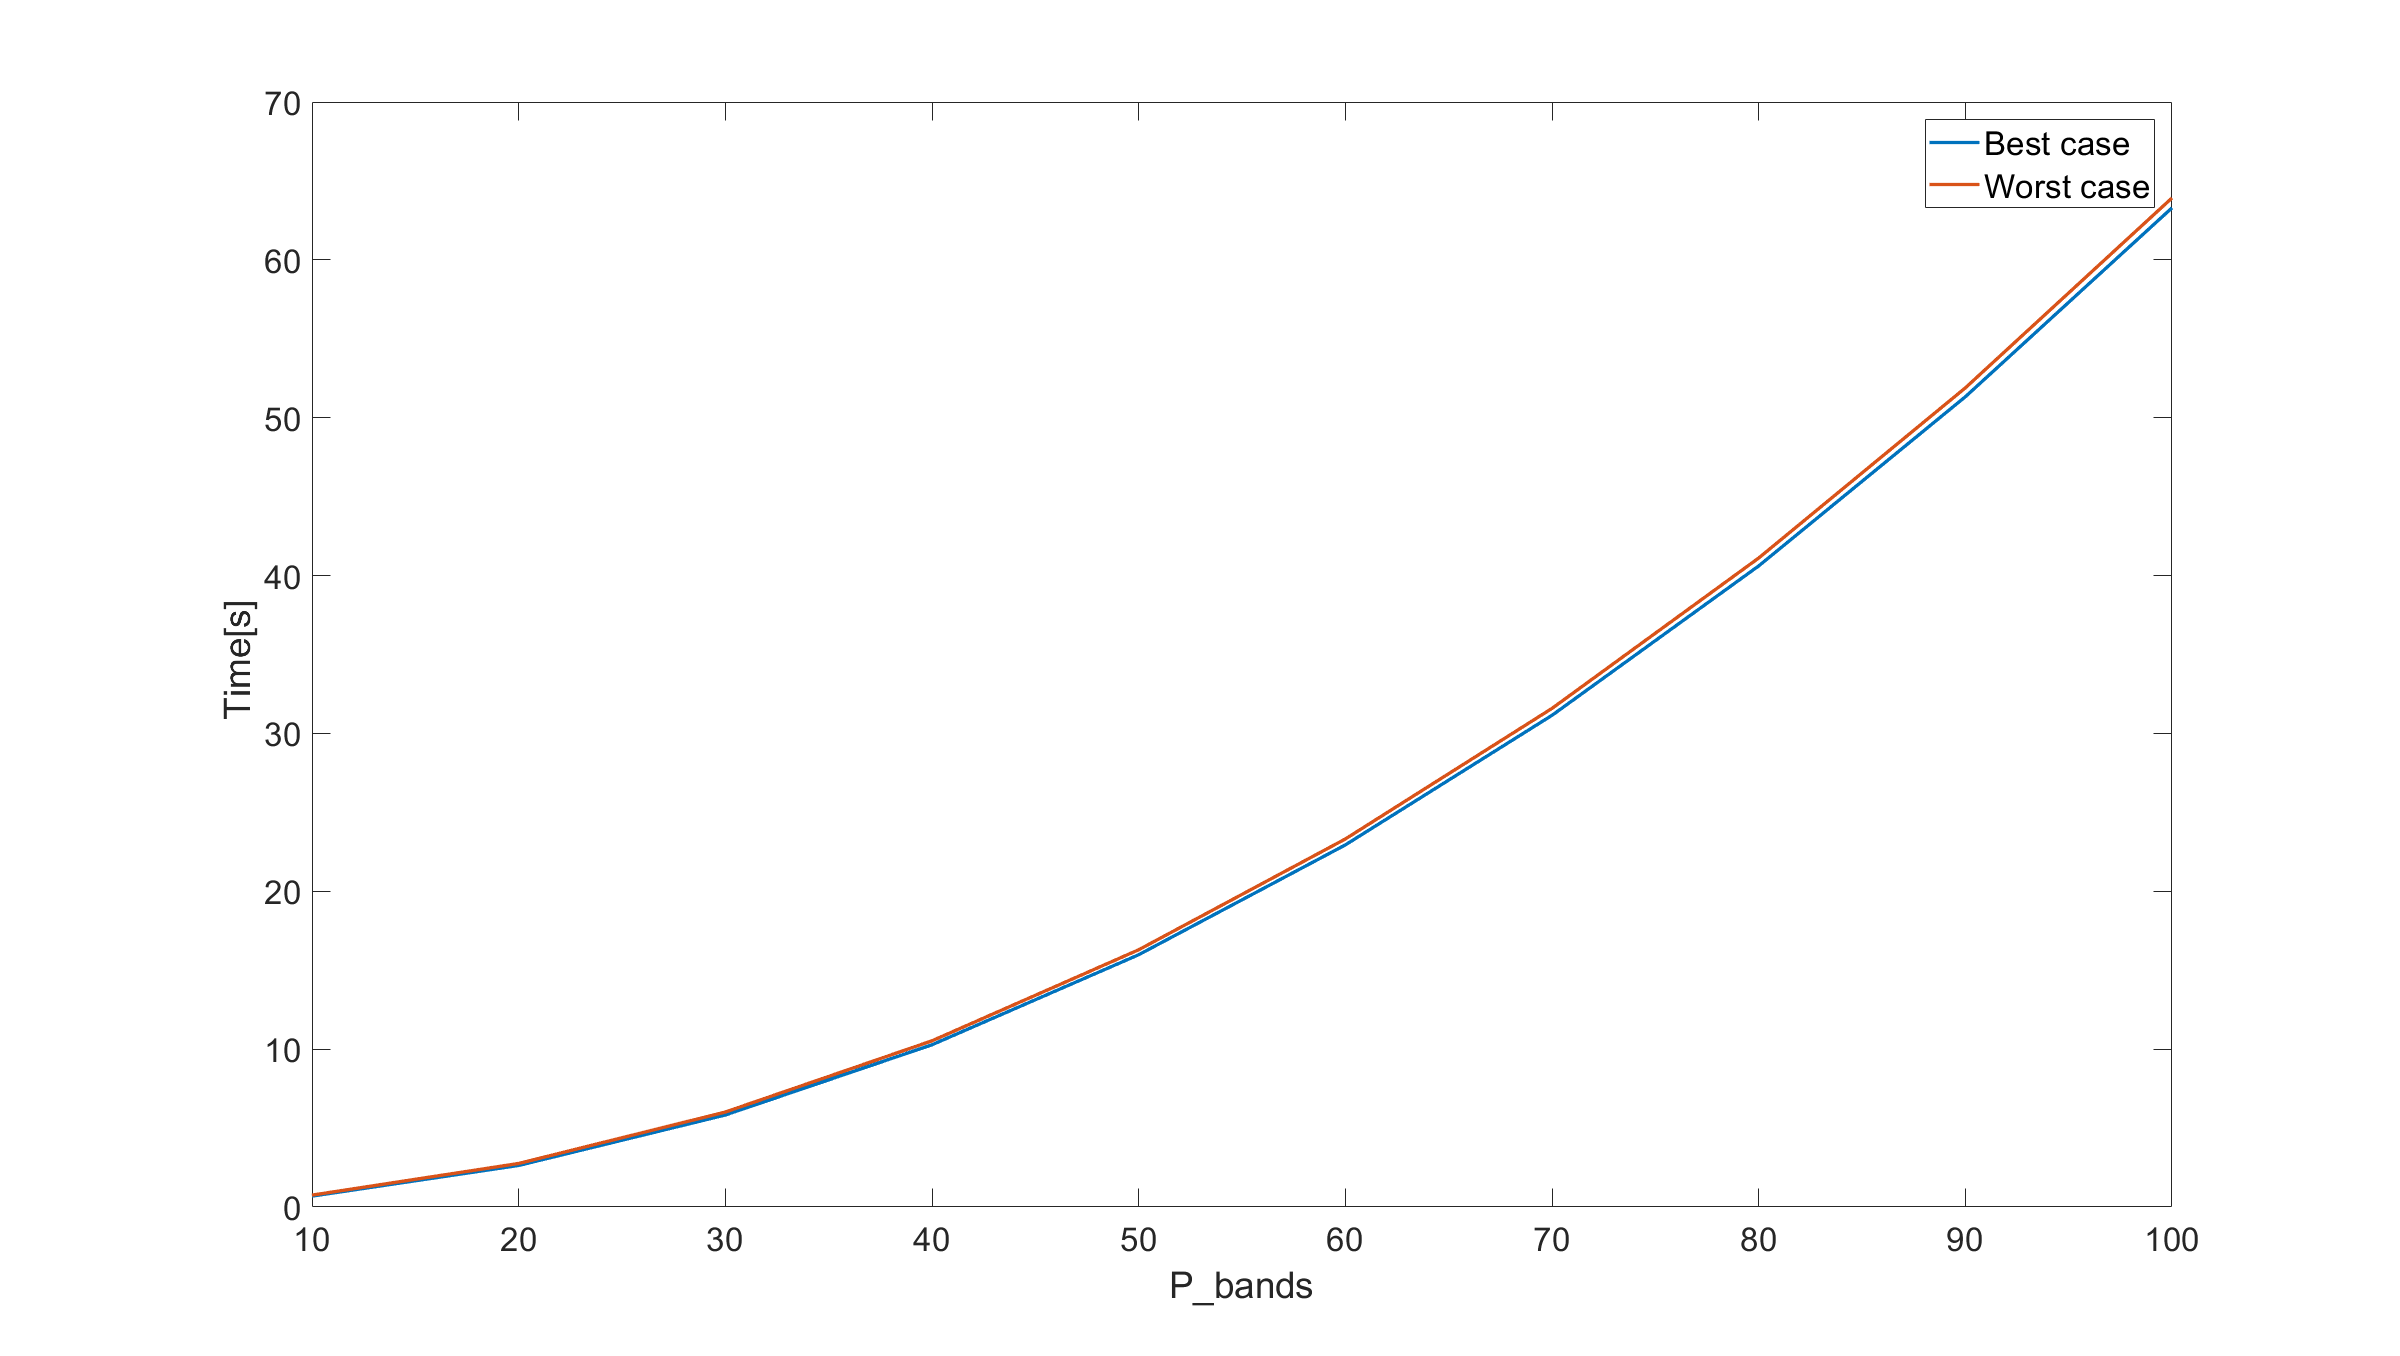
\includegraphics[scale=0.3]{images/estimated_execution_time_inverse_computation_in_seconds.png}}
  \caption{Estimated execution time for inverse matrix computation for an image of 1088x576, in seconds. The horizontal line marks the 54 second processing specification set by the SmallSat project.  } 
  \label{fig:estimated_time_inverse}
\end{figure}
%%\subsubsection{Inverse computation}
%%Estimated execution time backward elimination:
%%\begin{equation}
%%    B=\sum_{i=1}^{i=P_{BANDS}-1} i
%%\end{equation}

\subsection{Division}
\label{sec:division_implementation}
This section describes the implementation of division used in the Gauss-Jordan elimination.  The semantics used to described the division operation will be $C=B*\frac{1}{A}$ where $C,B$ and $A $ are integer variables. This corresponds to the inner loop operation for Last division shown in Figure \ref{fig:gauss_jordan_pseudocode}.


\subsubsection{Using division operator "/"}
\label{sec:division_operator}



%%\begin{figure}[H]
%%\centering
%%   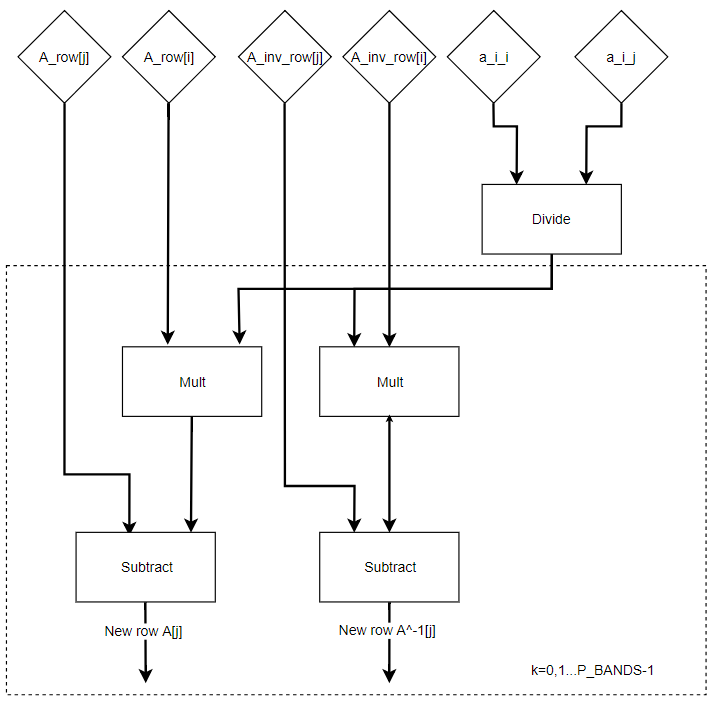
\includegraphics[scale=0.5]{images/inverse_hw/inverse_core_division_approach.PNG}
%%  \caption{Architecture of the \textbf{Elimination core} in Figure \ref{fig:top_level_inverse}, using division operator "/" for integer datatype in VHDL. $k$= $P\_BANDS$ modules marked by the dotted square is implemented in order to compute one row per clock cycle.  } 
%%  \label{fig:adaptive_shifting}
%%\end{figure}

To evaluate if division could be implemented by using the "/" operator, the $\textbf{Last division}$ block was synthesized, and the critical path evaluated, to see if the timing specification of 100 MHz operating frequency could be met. Results for different divisor -and-divident bit width is presented in Table \ref{tab:division_operator_logic_delays}. 


\begin{table}[H]
    \centering
    \begin{tabular}{c|c|c}
    \textbf{Bit width divisor and dividend} &\textbf{Logic delay[ns]}&\textbf{Max frequency[MHz] } \\
         32&72.498 &13.79 \\
         13 &19.726 &50.69\\
         10 & 16.032&62.37 \\
         8 & 12.74&78.49 \\
         6&9.530& 104.93\\
         
    \end{tabular}
    \caption{Synthesis results for ZedBoard Zynq Evaluation and Development Kit Z7020 for \textbf{Last division} shown in Figure \ref{fig:top_level_inverse}, implementing the product $C= B*\frac{1}{A}$. Bit width for factor $B$ is 32 bit.}
    \label{tab:division_operator_logic_delays}
\end{table}{}
%% Insert table here, with widths and delays

\subsubsection{Adaptive shifting}
\label{sec:adaptive_shifting}
        To avoid using the division operator the adaptive shifting approach shown in \ref{fig:adaptive_shifting} has been implemented. It approximates the divisor by an adaptive number of shift operations, as the divisor is not constant. To achieve this, the most significant bit(MSB) of the divisor is first checked to evaluate if the divisor is a negative number. If it is, the divisor is negated. The block \textbf{Find MSB} finds the MSB of the unsigned divisor. In parallel with this, $PIXEL\_DATA\_WIDTH*2-1$ numbers of shift operation processes shifts the unsigned divisor by $n\_shifts$=[1,2...$PIXEL\_DATA\_WIDTH*2-1$]. The remainders after shifting is sent to the \textbf{Choose best approximation} block. This block choose the best approximation depending upon the index of the MSB and the remainders after shifting. The best approximation to the divisor will be a shift operation by MSB or MSB+1 number of shifts. Each element of the row is then shifted in parallel to compute the approximate division in one clock cycle. If the divisor is a negative number, the row is negated before outputting data to register.
        \\
        The design shown in Figure \ref{fig:adaptive_shifting} was synthesized for Zedboard Zynq Evaluation and Development kit Z7020 to check timing. The max logic delay was $6.932$ns which gives a max operating frequency of 144.25 MHz, not accounting for net delay. 


The adaptive shifting will have an error of \textbf{FIND largest error.}. 

%\textbf{Mention the fact that r\_i\_i\_half is added before dividing. This is because of integer rounding in hardware/vivado}


\begin{figure}[H]
\centering
   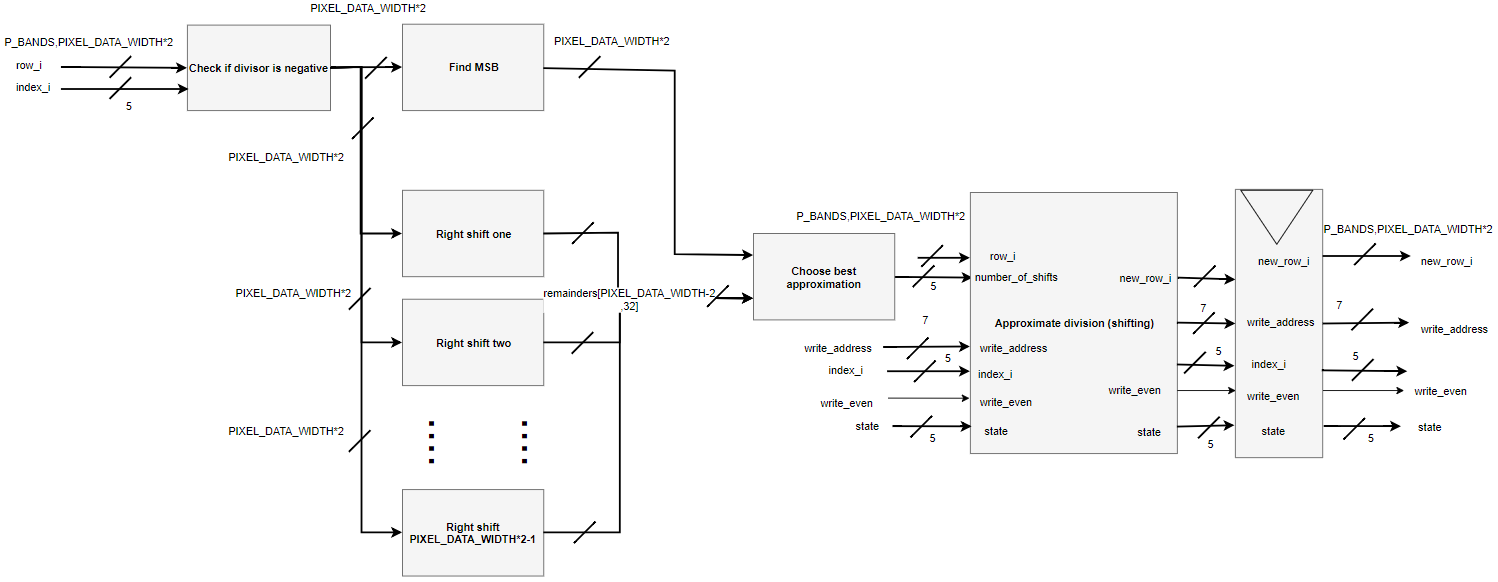
\includegraphics[scale=0.5]{images/approximate_division/last_division.PNG}
  \caption{Architecture of block \textbf{Last division}, approaching division with an adaptive number of shifts.   } 
  \label{fig:adaptive_shifting}
\end{figure}


\subsubsection{LUT approach}
\label{sec:LUT_division}
Instead of computing the division in the operation $C= B*\frac{1}{A}$, an approach based on the solution in \cite{cite:how_to_implement_division} was made. The approach utilizes LUTs to store the array $divisor\_inv$=$\frac{2^{DIV\_PRECISION}}{A}$, where $A=1,2...2^{DIV\_PRECISION}$ and $DIV\_PRECISION$ is the bit width of the divisor and the dividend. Instead of dividing by an integer $A$, $A$ is used as an index to look up in LUTs(number of LUTs depending upon $DIV\_PRECISION$) storing the $divisor\_inv$. $divisor\_inv(A)$ is then multiplied by $B$, which yields product $C$. $C$ is then right shifted $DIV\_PRECISION$ spaces. This can be seen in Equation \ref{LUT_operations}.

\begin{equation} \label{LUT_operations}
\begin{split}
C= shift\_right(B*\frac{2^{DIV\_PRECISION}}{A},DIV\_PRECISION)
\end{split}
\end{equation}

The code for inferring the LUTs for storage of $divisor\_inv$ is shown in Listing \ref{lst:lut_division}, examplified for DIV\_PRECISION=4.  

\lstinputlisting[caption={LUT division approach examplified for DIV\_PRECISION = 4.},label={lst:lut_division},style=customc]{code/lut_4_bit_example.vhd}

The architecture of the \textbf{Last division} block, utilizing this LUT approach, is shown in figure \ref{fig:top_last_division_lut_approach}. If choosing $DIV\_PRECISION$< $PIXEL\_DATA\_WIDTH*2$, an adaptive shifting approach is utilized. 
\\

\begin{figure}[H]
\hbox{\hspace*{-2cm}                                                           

   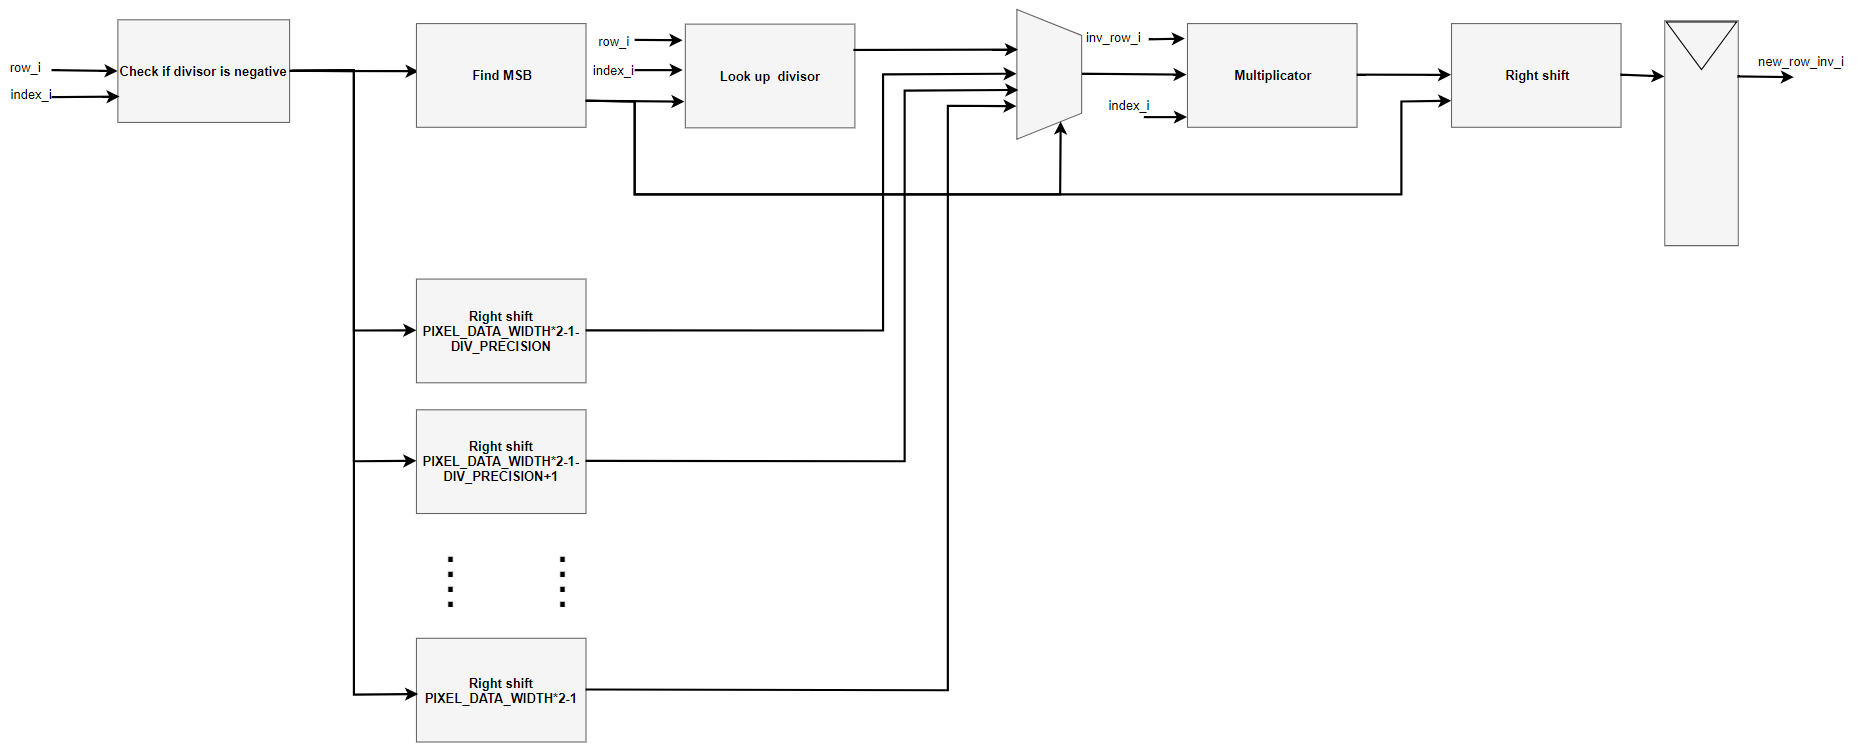
\includegraphics[scale=0.45]{images/approximate_division/top_last_division_lut_approach_dataflow.PNG}}
  \caption{Architecture of block \textbf{Last division}, computing division using the LUT approach.   } 
  \label{fig:top_last_division_lut_approach}
\end{figure}
\newpage
%\section{Results}
\chapter{Results}
\label{sec:results}
\section{Synthesis}
\label{sec:synthesis_results}
All synthesis results in this chapter are synthesized for $Pixel\_Data\_Width$ of 16, unless another value is 
especially mentioned. Results presented in this chapter are gathered from synthesis utilization reports.\\

The designs were synthesized in Vivado. As Zynq-7000 - Z7030/Z7035 was not available for synthesis, the Zedboard Evaluation and Development kit was used for synthesis. This kit contains less logic than the Z7030/Z7035. The kit contains only 220 DSPs. This leads to the the \textbf{ACAD inverse} over-utilizing DSPs when running synthesis for designs with $P\_bands$ $>=$ 20. When over-utilizing DSPs, the logic gets mapped to LUTs instead, as described in \cite{cite:dsp_overutilizing}, and will produce unusable synthesis results. Therefore; the design was synthesized for xc7k160tiffv676-2L, as this device contains 600 DSPs, in addition to having a similar architecture as the Zedboard (has Slice Registers and Slice LUTs, as opposed to CLB Registers and CLB LUTs). \textbf{ACAD correlation} also over-utilizes DSPs for $P\_bands$ >=60 and $Pixel\_data\_width$ = 16. Therefore, \textbf{ACAD correlation} is synthesized for xc7k160tiffv676-2L for $P\_bands$ >= 60 and $Pixel\_data\_width$ = 16.\\

Timing results when synthesizing for xc7k160tiffv676-2L is not considered usable, as the device logic is different to the Zedboard. The Zedboard contains an Artix-7 device, which is a slower device than the Z-7030/Z-7035, which are Kintex-7 devices. Designs that meets timing demands for the Zedboard will therefore also most likely meet timing requirements for the Z-7030/Z-7035 devices. In addition to this, the initial test prototype is to be implemented on a Zedboard. As such, it is valuable to see if the design meet timing when running on Zedboard. Therefore, only timing results from synthesis on the Zedboard Evaluation and development kit is presented. 



\subsection{Shiftregister}
\textbf{Shiftregister} was synthesized for $P\_bands$= [10, 20, 30, 40, 50, 60, 70, 80, 90, 100]. Number of synthesized Slice registers and Slice LUTs are shown in Figure \ref{fig:primitives_shiftregister}. 

\begin{figure}[H]

\hbox{\hspace*{-2cm}                                                           
   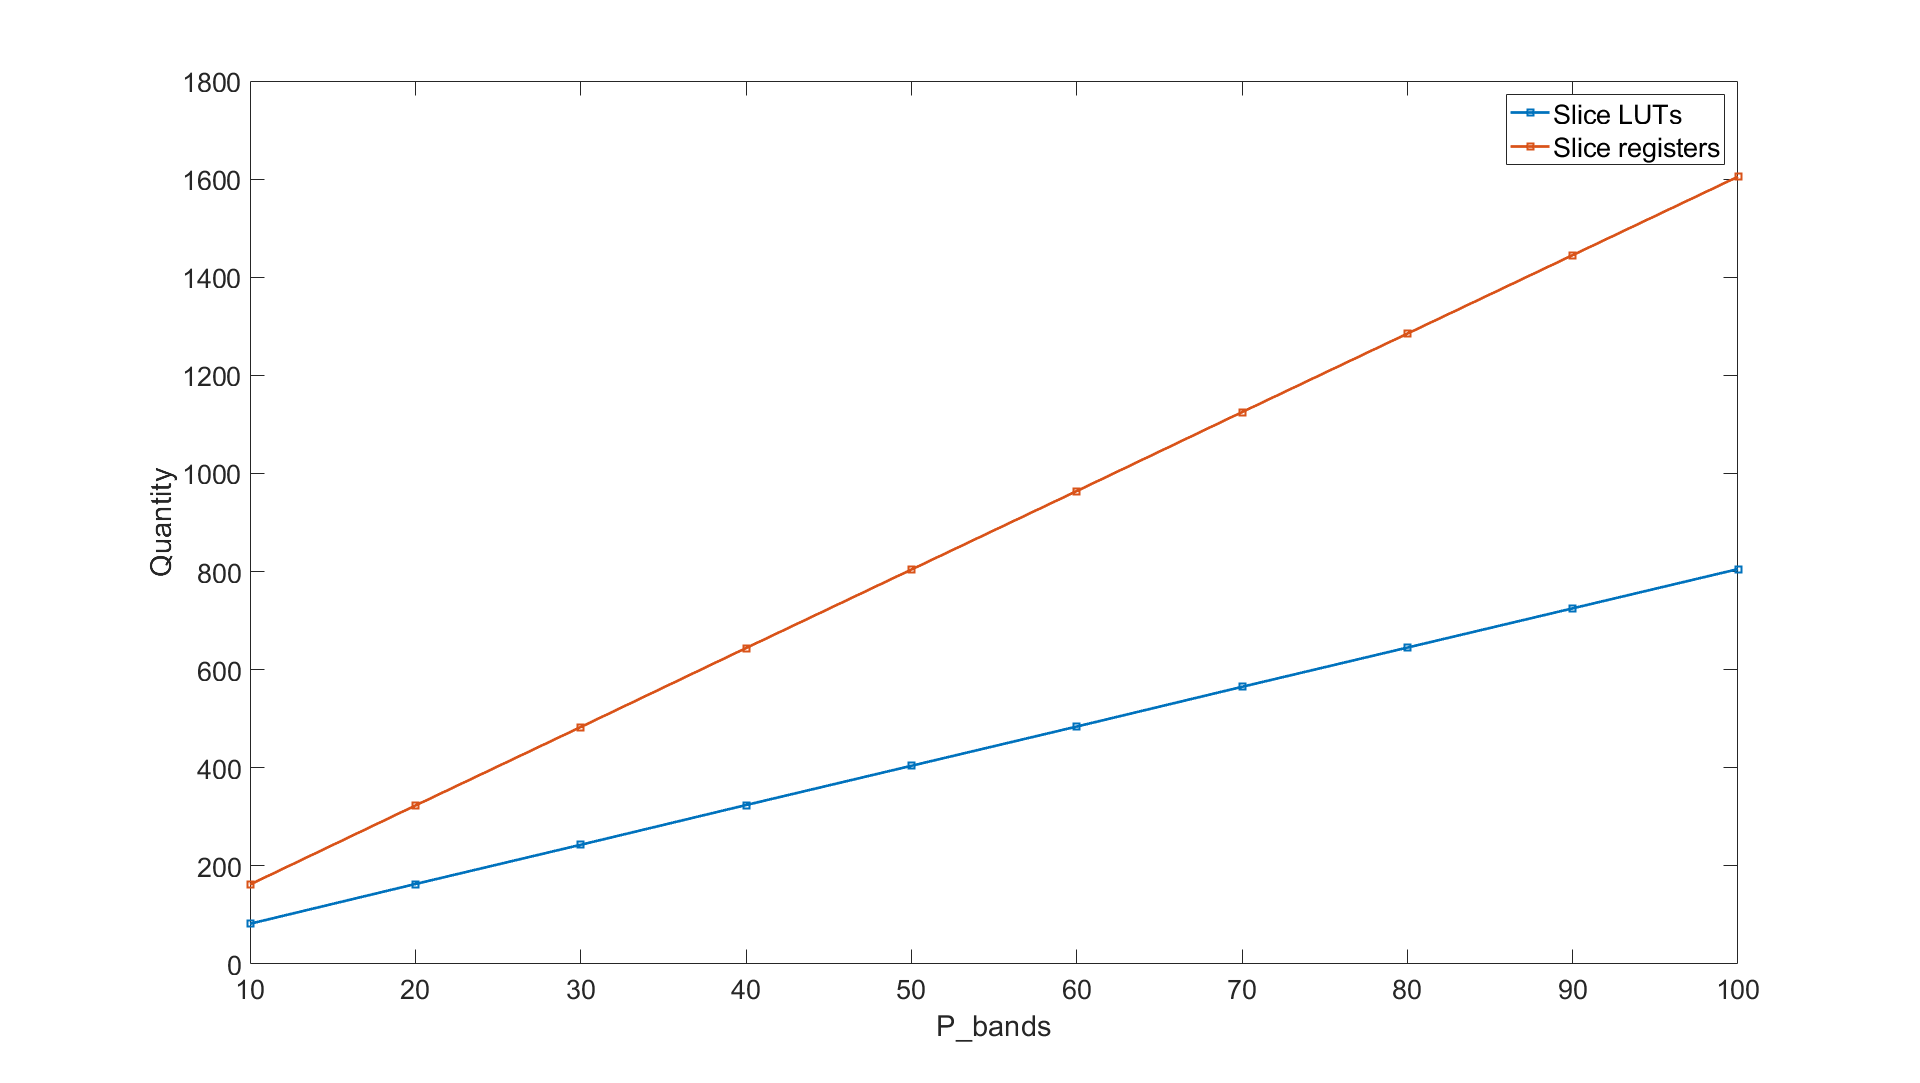
\includegraphics[scale=0.3]{images/syntese_resultat/shiftregister.png}}
  \caption{\textbf{Shiftregister} synthesis results.  } 
  \label{fig:primitives_shiftregister}
\end{figure}

\subsection{ACAD correlation}

The design was synthesized for $P\_bands$= [10, 20, 30, 40, 50, 60, 70, 80, 90, 100]. Figure \ref{fig:primitves_correlation}  shows the number of synthesized BRAM36E1 and DSP48E1. Figure \ref{fig:luts_and_regs_corr} shows number of synthesized Slice Registers and Slice LUTs as a function of $P\_bands$.

\begin{figure}[H]

\hbox{\hspace*{-2cm}                                                           
   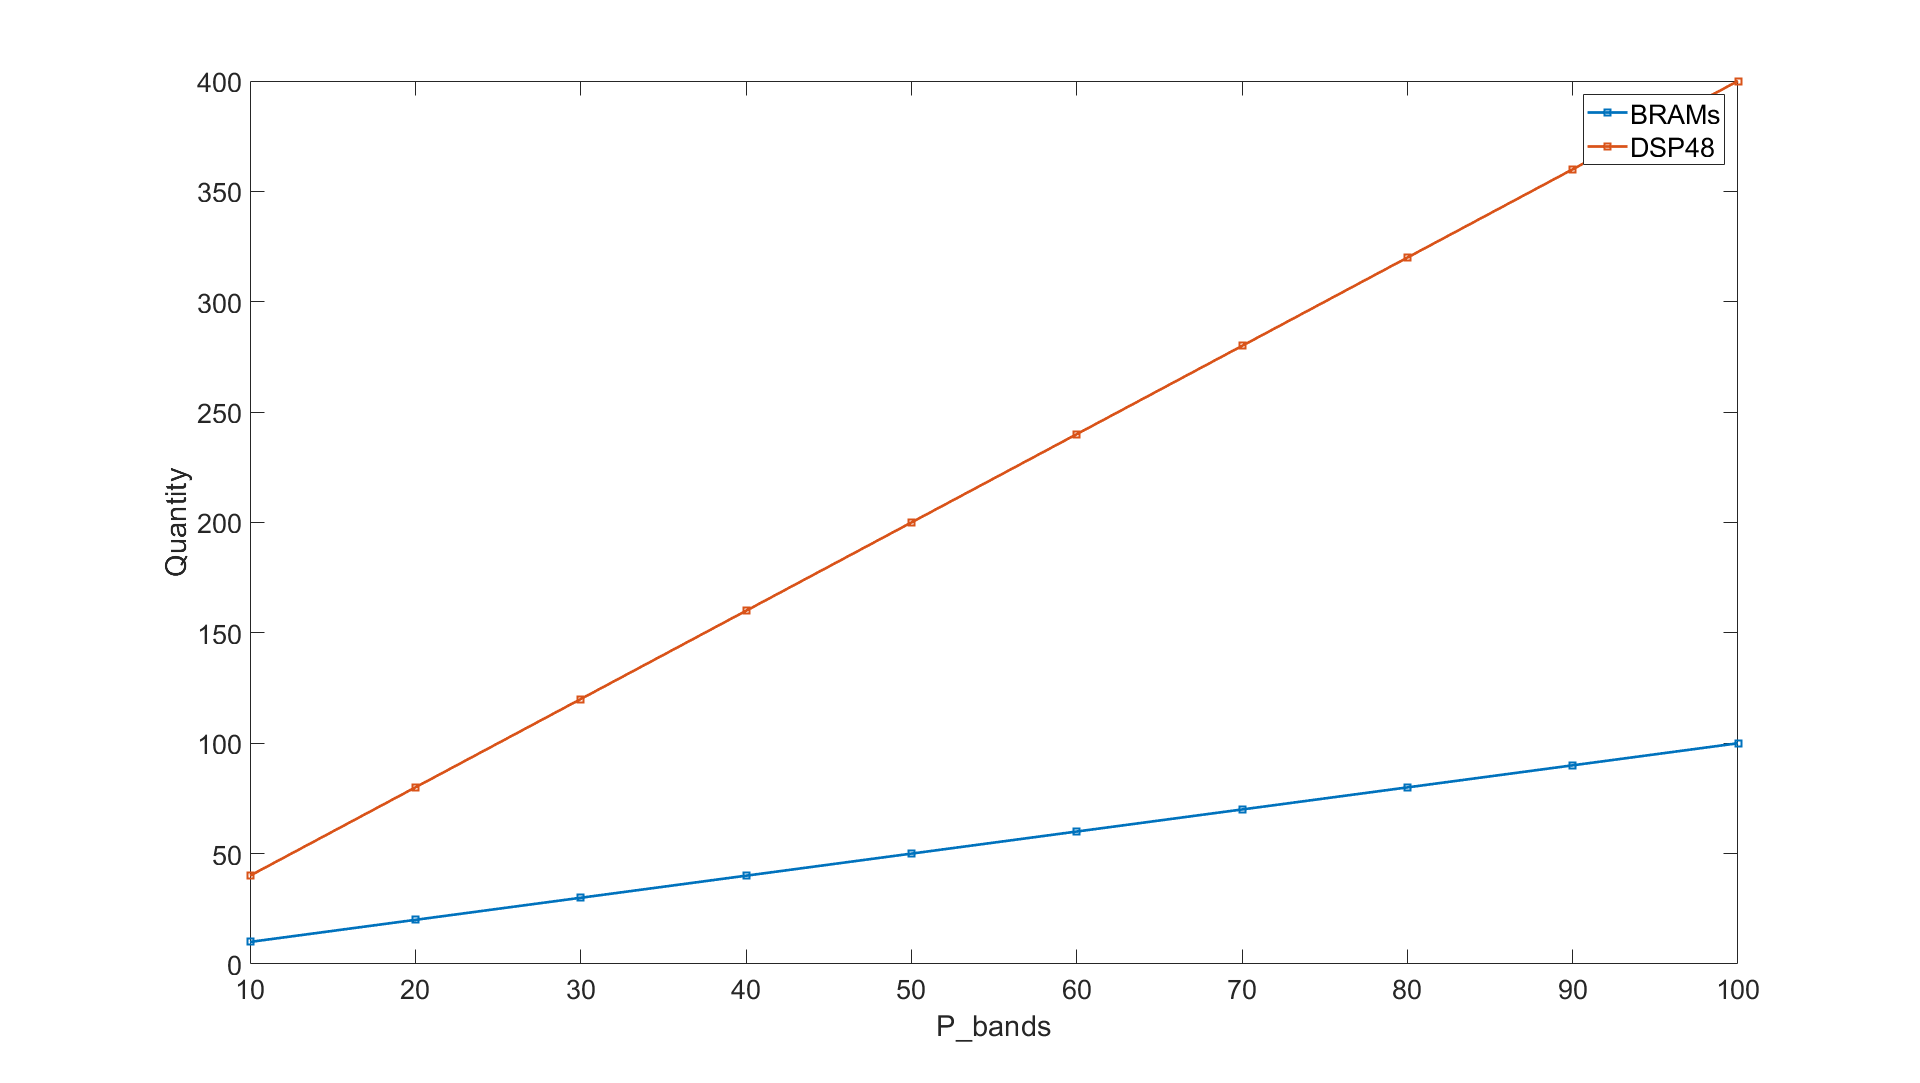
\includegraphics[scale=0.3]{images/number_of_BRAMS_and_DSP48_correlation_module.png}}
  \caption{Number of synthesized BRAM36E1 and DSP48E1 as a function of $P\_bands$ for the \textbf{ACAD correlation} block.  } 
  \label{fig:primitves_correlation}
\end{figure}


\begin{figure}[H]

\hbox{\hspace*{-2cm}                                                           
   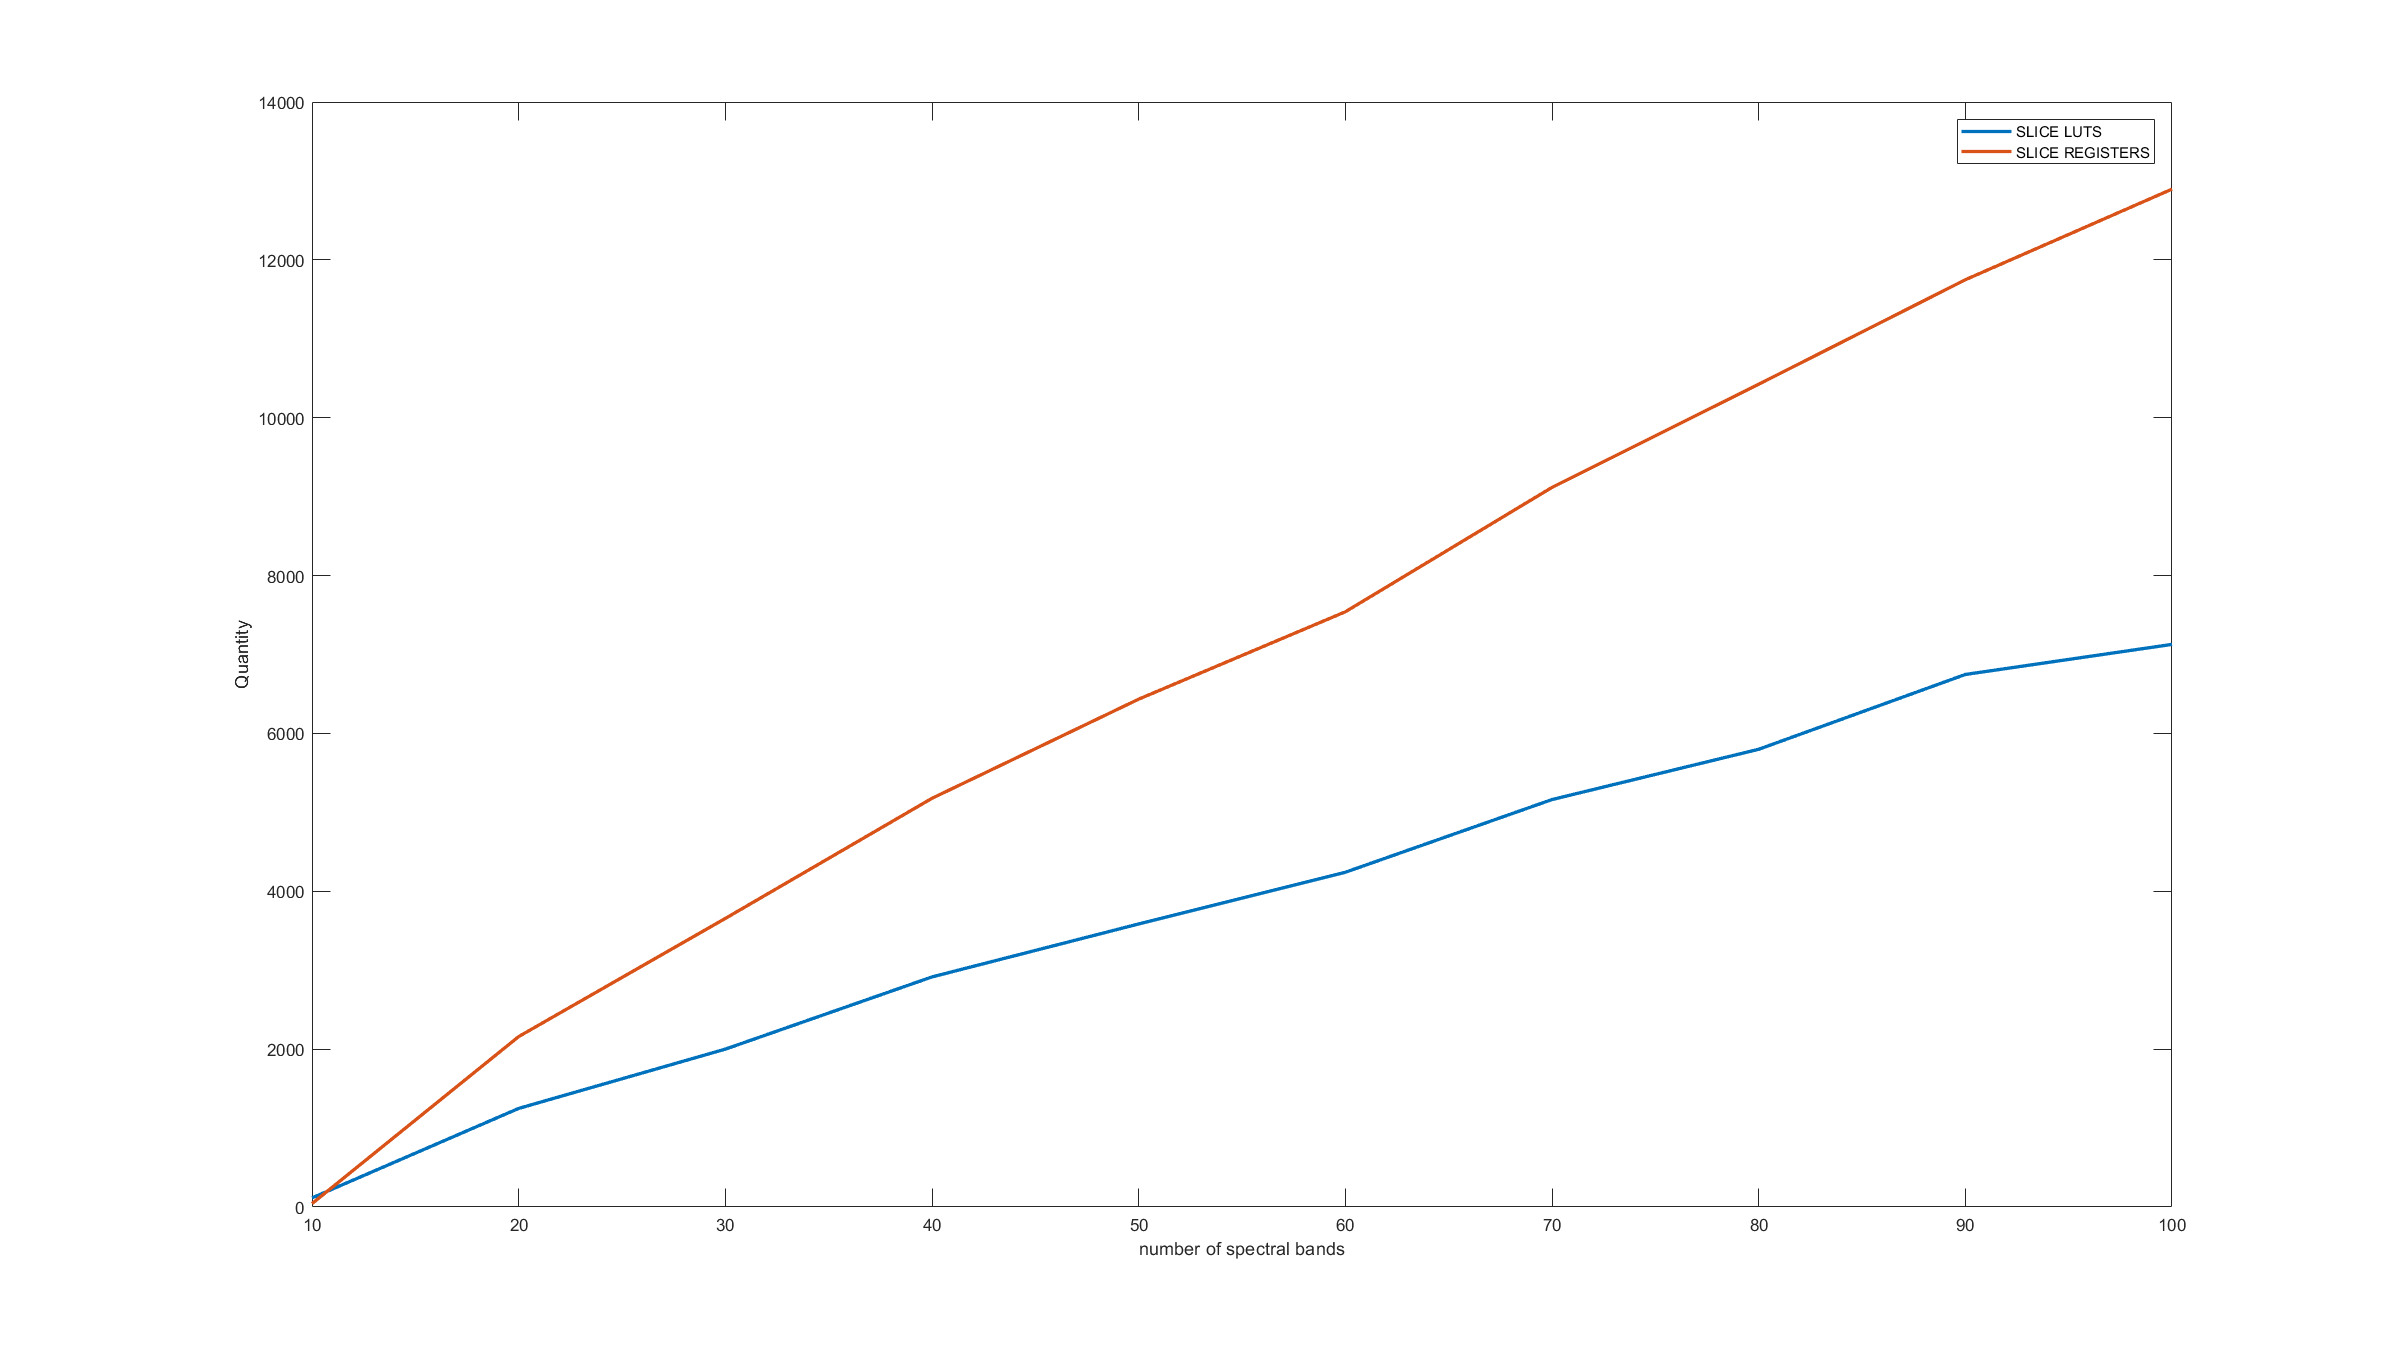
\includegraphics[scale=0.3]{images/correlation_luts_and_registers.png}}
  \caption{Number of synthesized Slice Registers and Slice LUTs as a function of $P\_bands$ for the \textbf{ACAD correlation} block. } 
  \label{fig:luts_and_regs_corr}
\end{figure}

\subsubsection{$Pixel\_data\_width$ = 10}
 As \textbf{ACAD correlation} inferred a large number of DSPs, $Pixel\_data\_width$ was lowered to see if the number of DSPs inferred would be lowered. The design inferred DSPs for $Pixel\_data\_width$ >= 11, but for $Pixel\_data\_width$ = 10 the synthesis tool did not inferr any DSPs. Instead the logic was mapped to LUTs. Number of BRAMs synthesized are unchanged when varying $Pixel\_data\_width$. Number of LUTs and registers synthesized are shown in Figure  \ref{fig:correlation_luts_and_registers_10}. 
 
\begin{figure}[H]

\hbox{\hspace*{-2cm}                                                           
   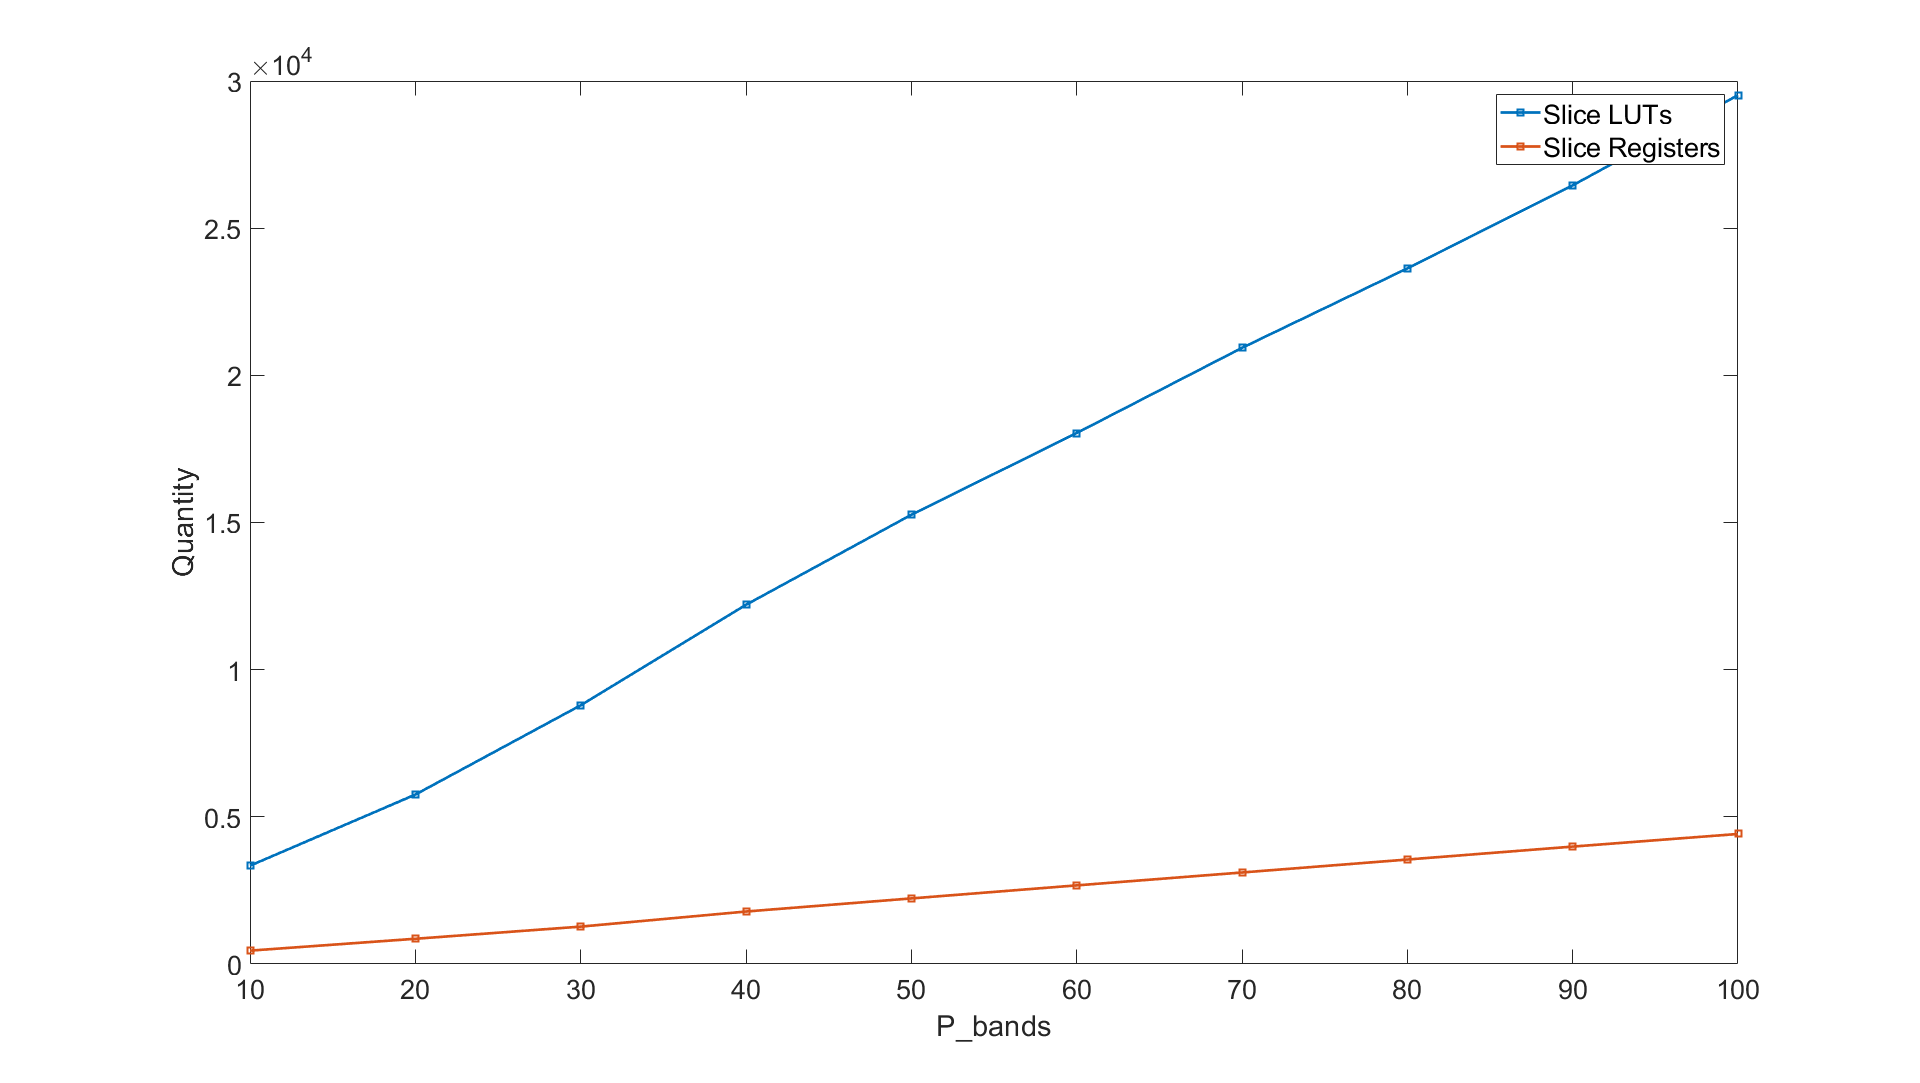
\includegraphics[scale=0.3]{images/syntese_resultat/acad_correlation_using_pixel_data_with_10_luts_and_registers.png}}
  \caption{Number of synthesized Slice Registers and Slice LUTs as a function of $P\_bands$ for the \textbf{ACAD correlation} block for $Pixel\_data\_with$ =10. } 
  \label{fig:correlation_luts_and_registers_10}
\end{figure}
 
 

\subsection{ACAD inverse}

\textbf{ACAD inverse} was synthesized using the three different division-approaches.  Number of BRAMs synthesized for the three approaches are equal, as shown in Figure \ref{fig:brams_inverse}. 


\begin{figure}[H]

\hbox{\hspace*{-1cm}                                                           
   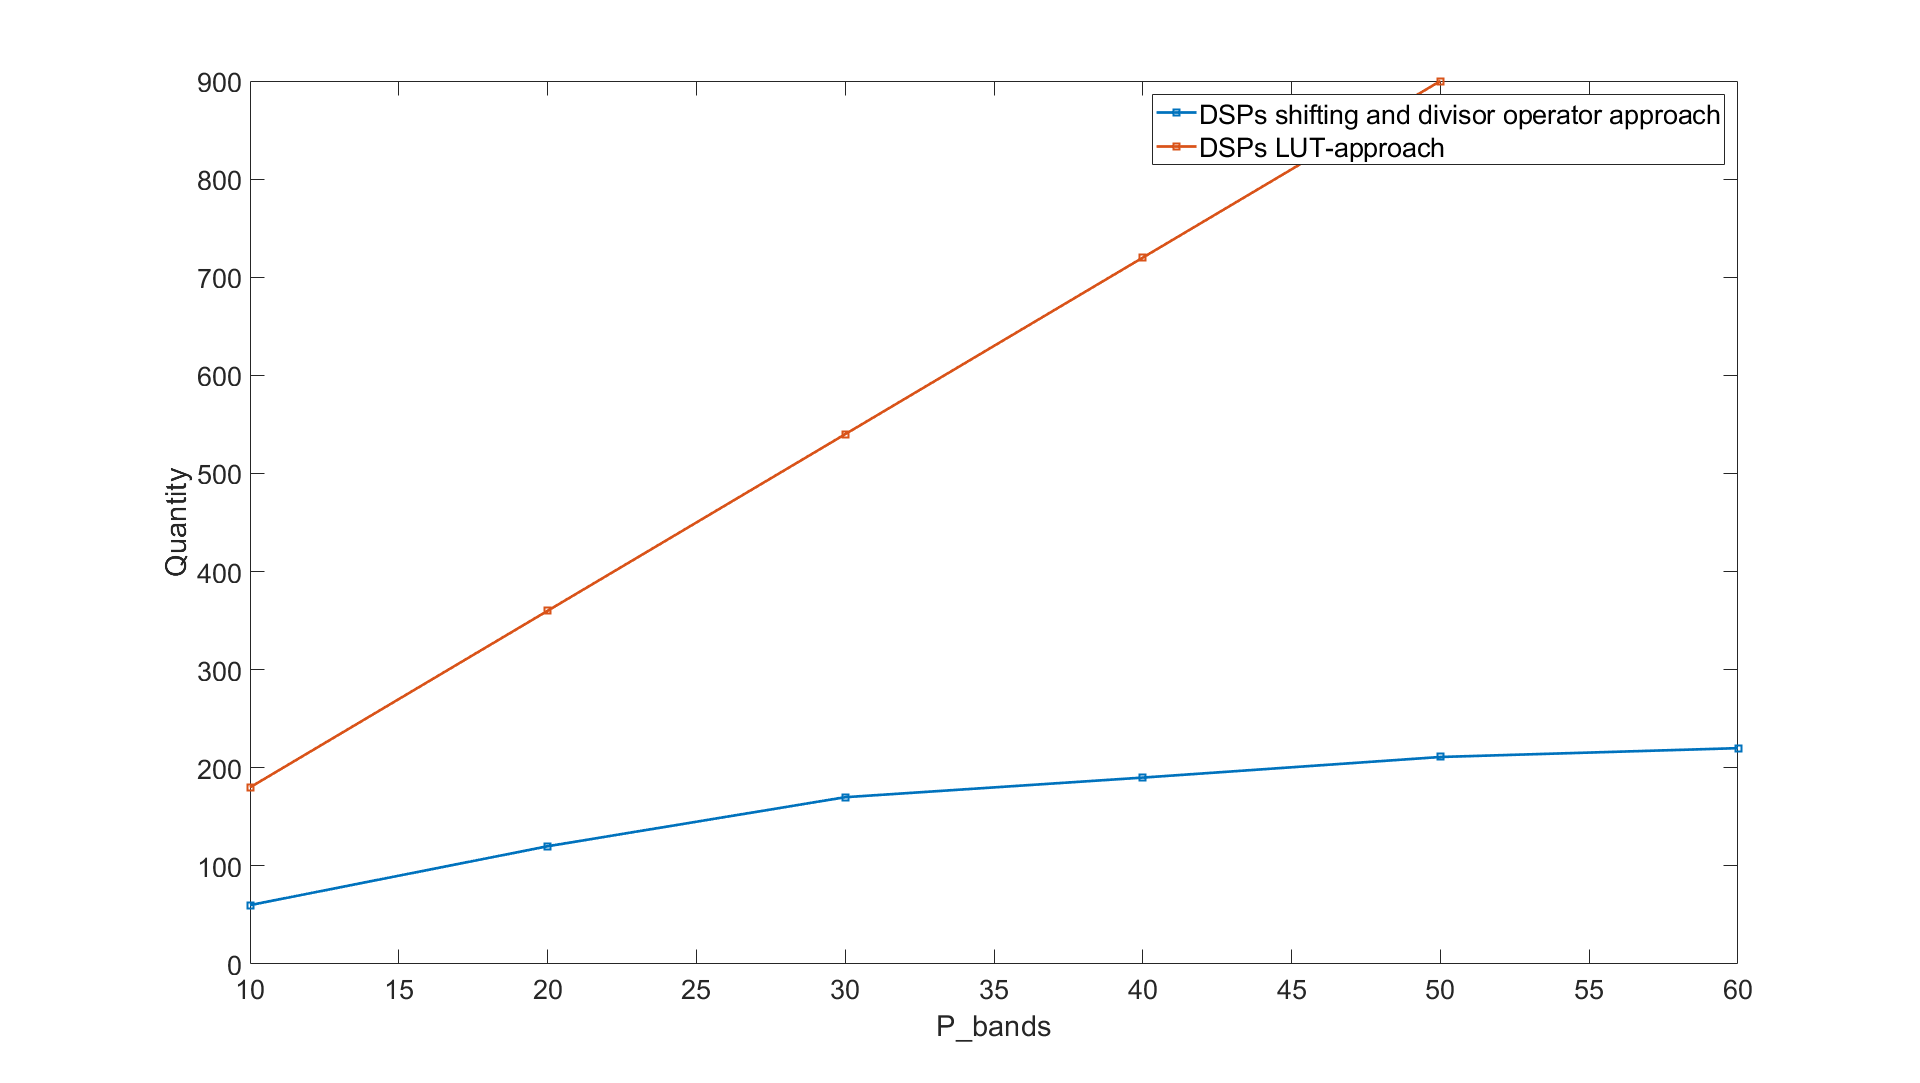
\includegraphics[scale=0.27]{images/syntese_resultat/inverse/number_of_dsps.png}}
  \caption{Number of DSP48E1 synthesized for the \textbf{Inverse} block. } 
  \label{fig:dsps_inverse}
\end{figure}


\begin{figure}[H]

\hbox{\hspace*{-1cm}                                                           
   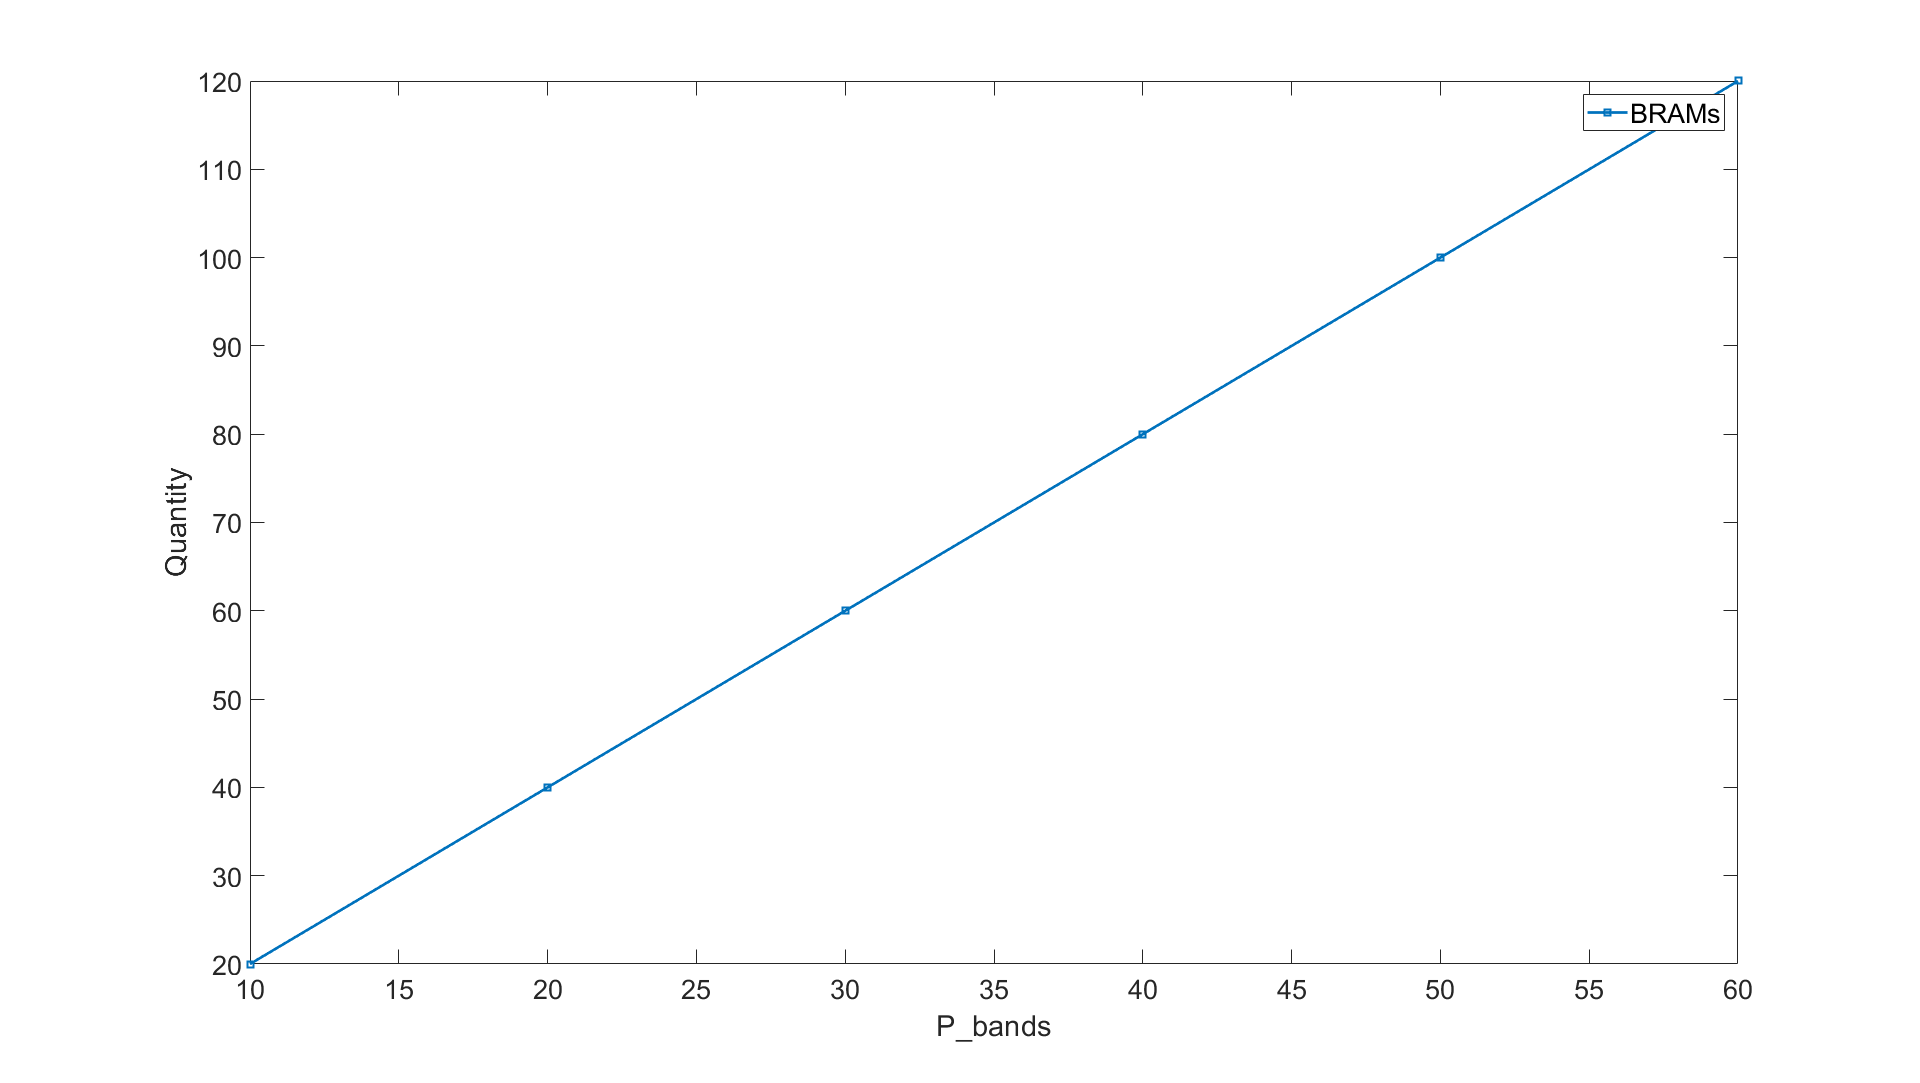
\includegraphics[scale=0.27]{images/syntese_resultat/inverse/brams.png}}
  \caption{Number of BRAMs synthesized for the \textbf{Inverse} block. } 
  \label{fig:brams_inverse}
\end{figure}


\begin{figure}[H]

\hbox{\hspace*{-2cm}                                                           
   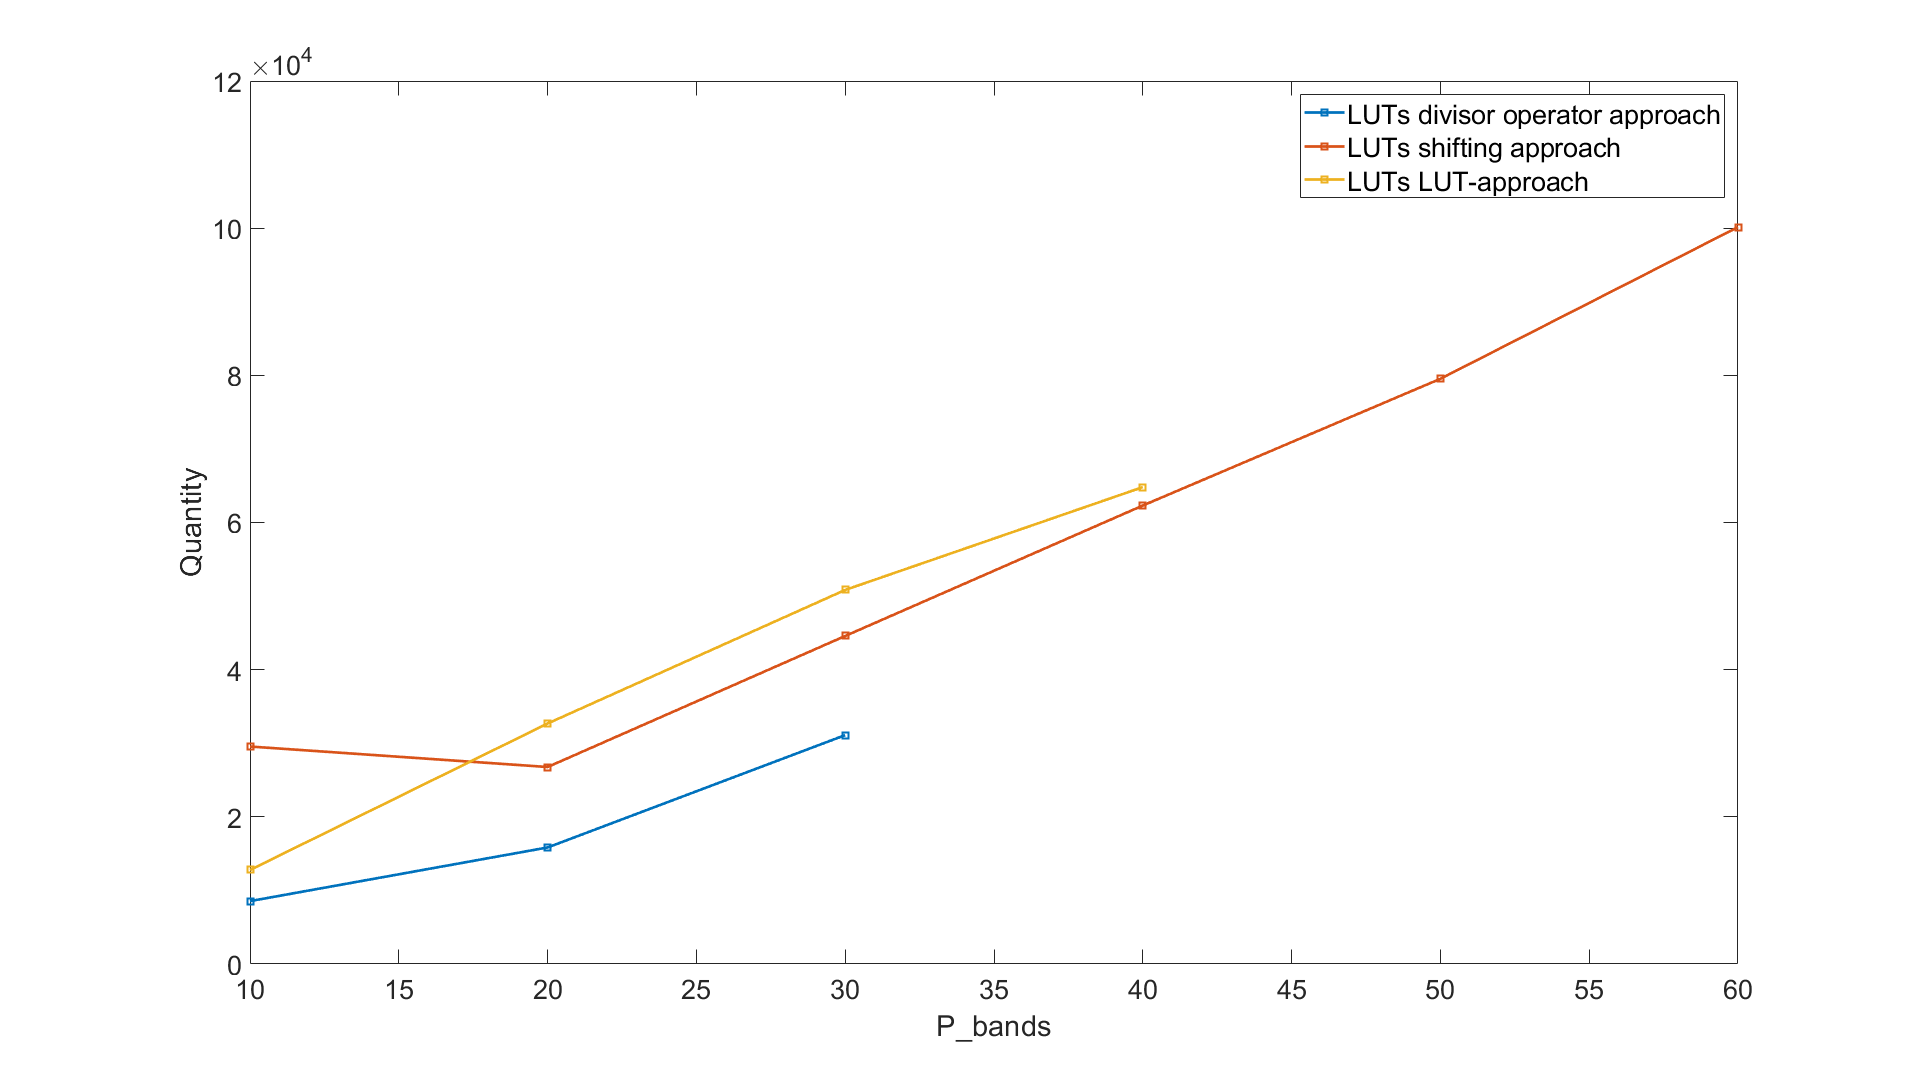
\includegraphics[scale=0.3]{images/syntese_resultat/inverse/number_of_luts.png}}
  \caption{Number of LUTs synthesized for the \textbf{Inverse} block. } 
  \label{fig:luts_inverse}
\end{figure}


\begin{figure}[H]

\hbox{\hspace*{-2cm}                                                           
   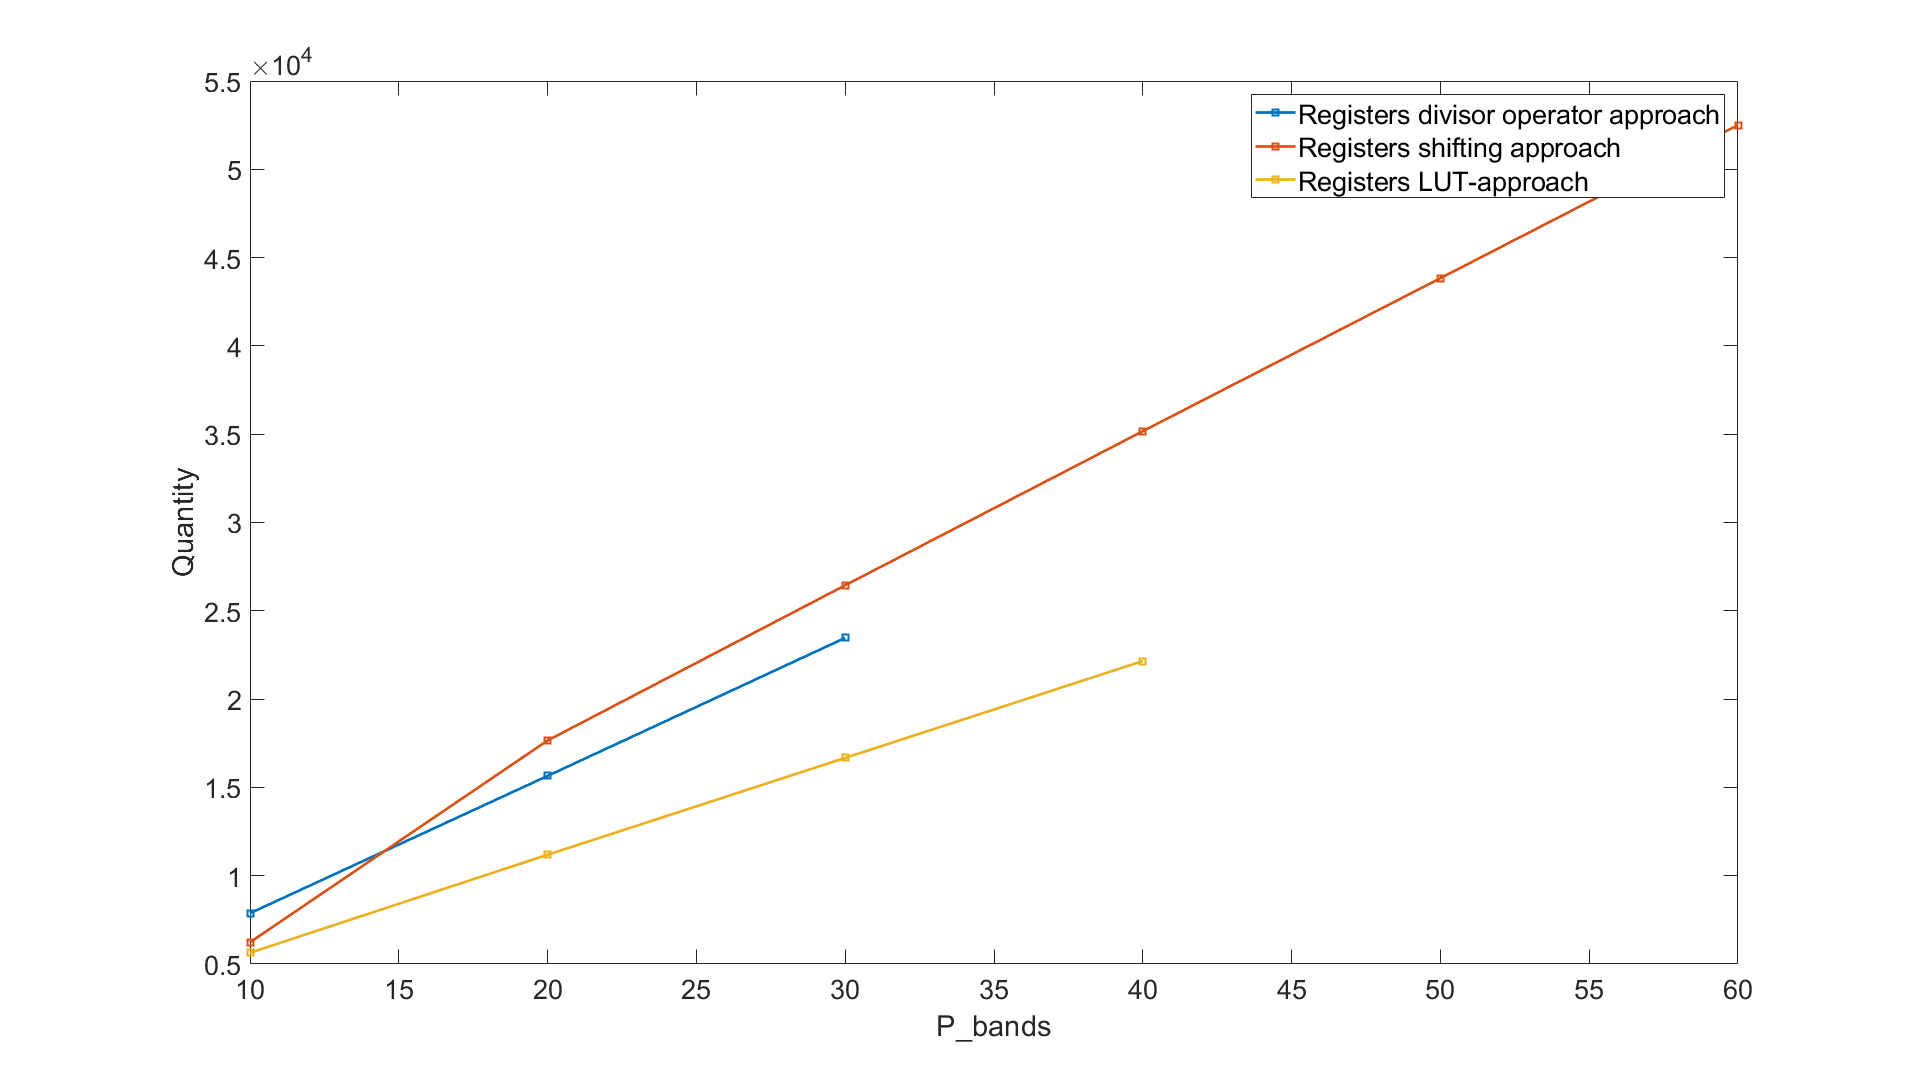
\includegraphics[scale=0.3]{images/syntese_resultat/inverse/number_of_registers.png}}
  \caption{Number of registers synthesized  for the \textbf{Inverse} block.. } 
  \label{fig:registers_inverse}
\end{figure}




%\subsubsection{LUTs and registers}
%\label{sec:synthesis:luts_and_registers_inverse}
%Synthesis results for the first and the second implementation approach of the Gauss-Jordan elimination is shown in Figure \ref{fig:synthesis_result_naive_inverse}.
%
%\begin{figure}[H]
%\hbox{\hspace*{-2cm}                                                           
%
%   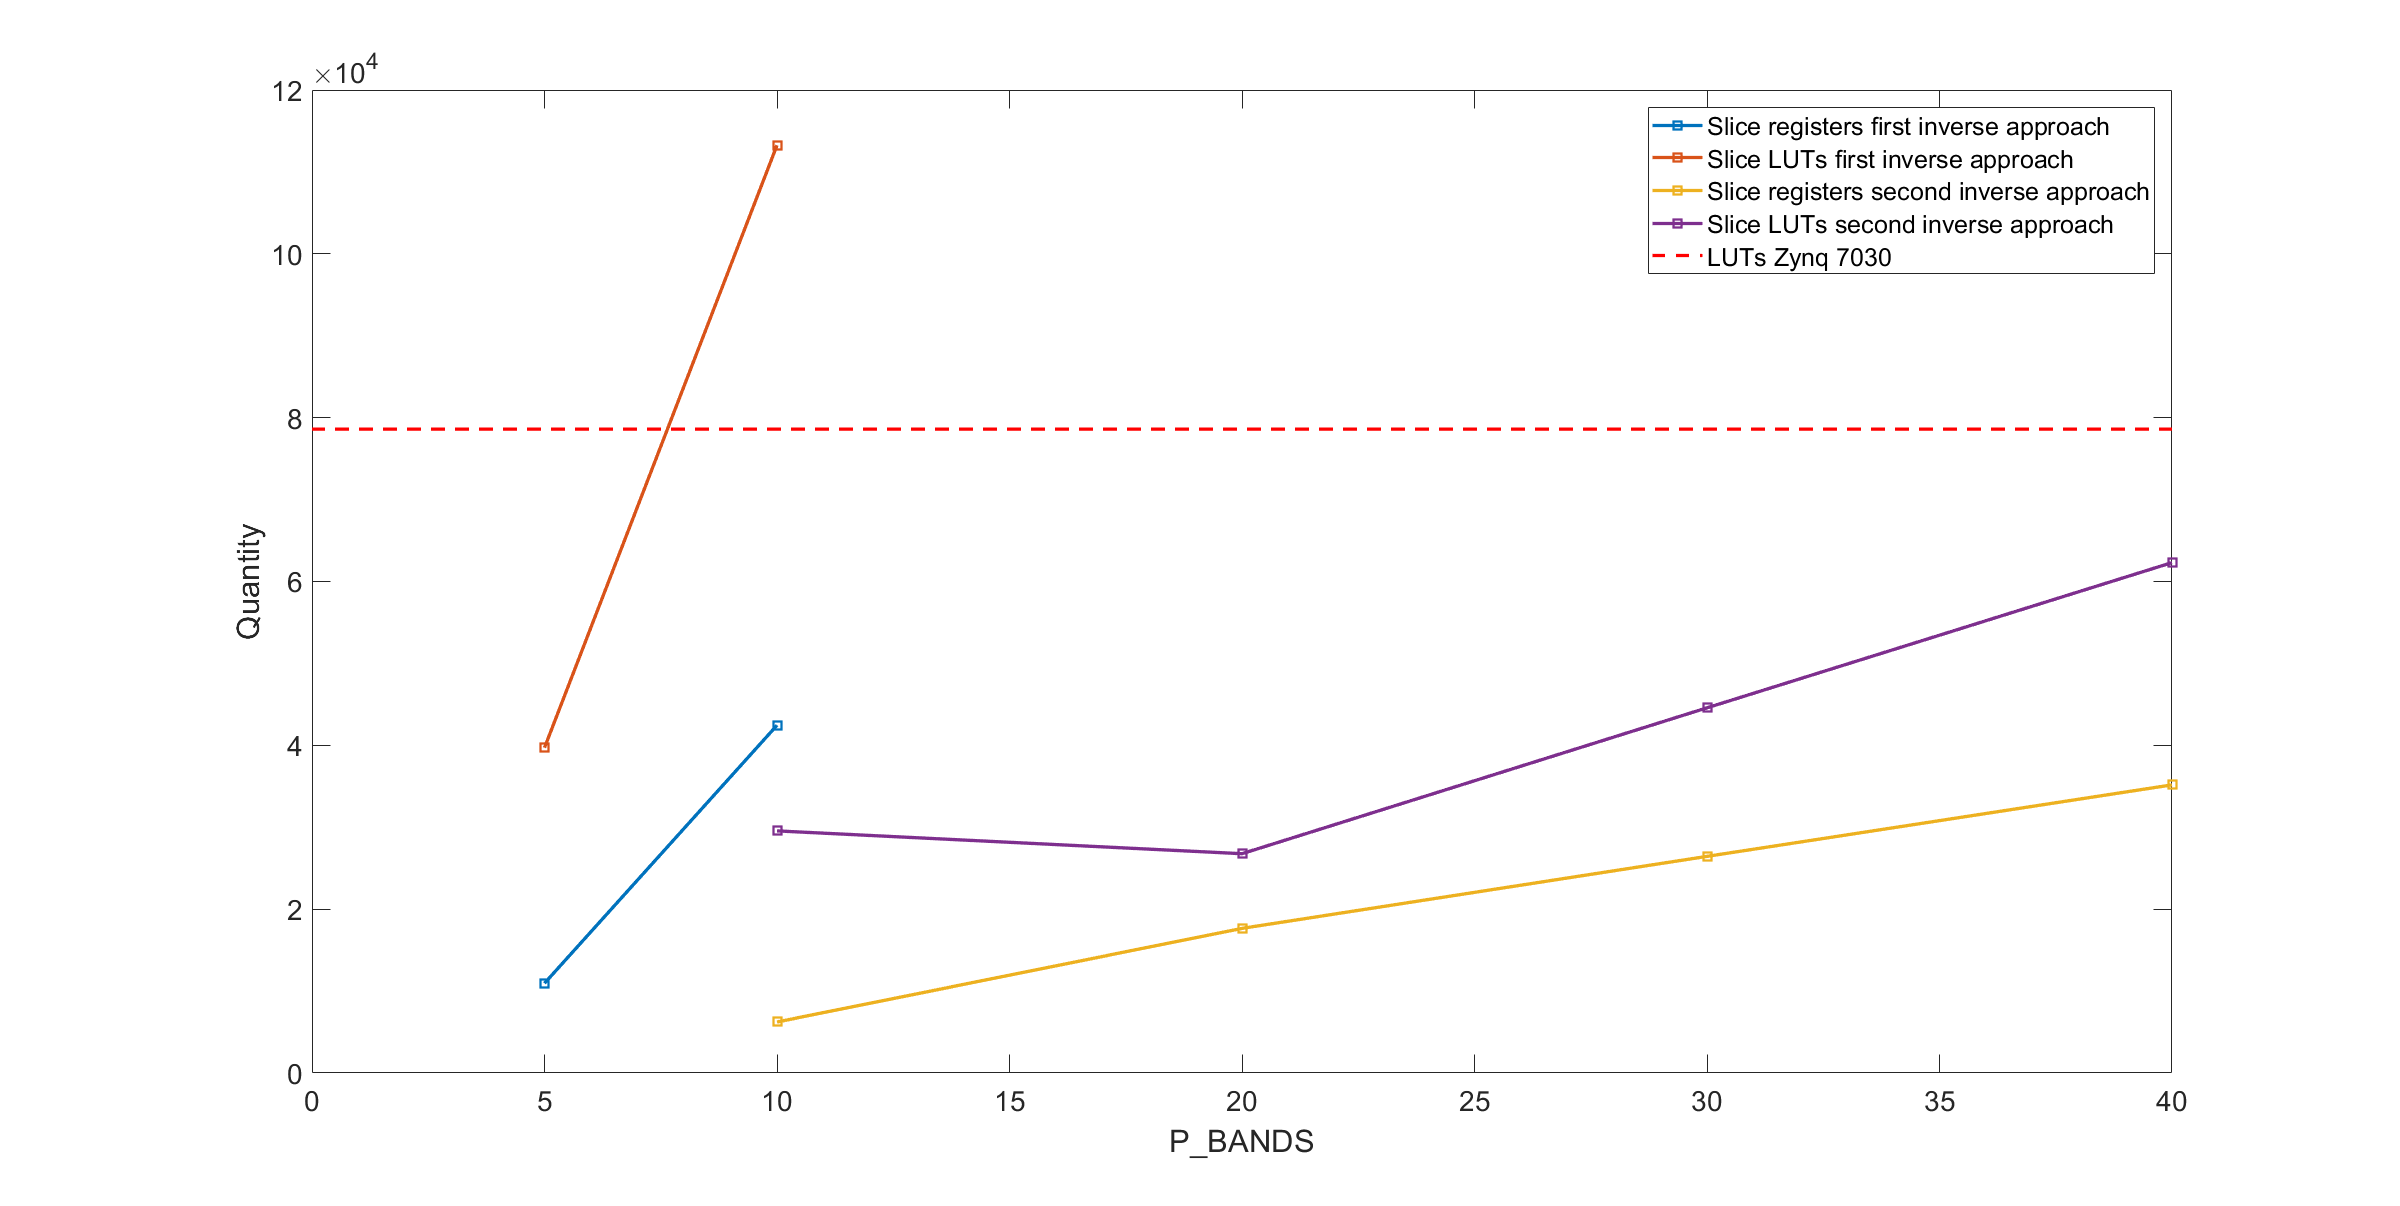
\includegraphics[scale=0.3]{images/inverse_hw/inverse_matrix_luts_and_registers.png}}
%  \caption{Synthesis result for the first and second Gauss-Jordan implementation approach, showing number of LUTs and registers synthesized.  } 
%  \label{fig:synthesis_result_naive_inverse}
%\end{figure}

\subsection{Timing results}
To check if the design met timing, the WNS of the synthesized designs was checked. The target clock frequency was set to 100 MHz. 
\subsubsection{WNS ACAD Correlation}
\textbf{ACAD correlation} was synthesized for $P\_bands$ = [10, 20, 30, 40, 50] and $Pixel\_data\_width$ = 16 on the ZedBoard Zynq Evaluation and Development Kit. The timing results are presented in Table \ref{tab:wns_correlation}.

\begin{table}[H]
    \centering
    % \resizebox{1.\textwidth}{!}{
    \begin{tabular}{c|c}
    \textbf{$P\_bands$} &\textbf{WNS [ns]} \\
    10 & 4.235 \\
    20 & 0.721\\
    30 &1.446\\
    40 & 0.845 \\
    50 & 0.509 \\
    \end{tabular}%}
    \caption{Timing results for \textbf{ACAD correlation} $Pixel\_data\_width$ = 16.}
    \label{tab:wns_correlation}
\end{table}

\textbf{ACAD correlation} was synthesized for $P\_bands$ = [10, 20, 30, 40, 50, 60, 70, 80, 90] and $Pixel\_data\_width$ = 10 on the ZedBoard Zynq Evaluation and Development Kit. The timing results are presented in Table \ref{tab:wns_correlation_10}.
\begin{table}[H]
    \centering
    % \resizebox{1.\textwidth}{!}{
    \begin{tabular}{c|c|c|c}
    \textbf{$P\_bands$} &\textbf{WNS [ns]}& \textbf{Net delay [ns]}& \textbf{Logic delay [ns]} \\
    10 &-3.074 & 7.860 & 5.078 \\
    20 & -3.309& 7.868 & 5.305 \\
    30 & -3.109 & 6.732 & 6.241\\
    40 & -3.319 & 7.698 & 5.485 \\
    50 & -3.324 & 7.703 & 5.485 \\
    60 & -3.331 & 7.518 & 5.677 \\
    70 & -4.923 & 8.563 & 6.224 \\
    80 & -4.881 & 8.521 & 6.224 \\
    90 & -5.224 & 9.373 & 5.735 \\
    
    \end{tabular}%}
    \caption{Timing results for \textbf{ACAD correlation} $Pixel\_data\_width$ = 10.}
    \label{tab:wns_correlation_10}
\end{table}


\subsubsection{WNS division operator}
Implementing division by the use of the division operator "/" yielded the timing results presented in Table \ref{tab:division_operator_wns} when synthesizing block \textbf{Last division}, computing the product $C= B*\frac{1}{A}$. Width of $B$ is 32 bit. The design was synthesized for dividend and divisor data width of 32, 8, 6 and 5, with a target clock constraint of 100 MHz. The target device was the Zedboard Zynq Evaluation and Development kit. 
\begin{table}[H]
    \centering
     \resizebox{1.\textwidth}{!}{
    \begin{tabular}{c|c|c}
    \textbf{Data width divisor and dividend} &\textbf{WNS [ns]}&\textbf{Max frequency [MHz] } \\
         32&-80.524&11.046 \\
         8 & -11.776&45.934 \\
         6&-7.071& 58.578\\
         5 & -5.730&63.572 \\
         
    \end{tabular}}
    \caption{Synthesis results for ZedBoard Zynq Evaluation and Development Kit for \textbf{Last division} using division operator "/".}
    \label{tab:division_operator_wns}
\end{table}
\subsubsection{Worst Negative Slack Adaptive Shifting}
 The design shown in Figure \ref{fig:adaptive_shifting} was synthesized for Zedboard Zynq Evaluation and Development kit Z7020 to check timing for $P\_bands$= [10, 20, 30, 40, 50, 60]. The worst WNS was 2.034 ns, which yields $f_{max}$ of \approx 125 MHz. 
 
 %The max logic delay was $6.932$ns which gives a max operating frequency of 144.25 MHz, not accounting for net delay. 
 
 
 \subsubsection{Worst Negative Slack LUT approach}
 The \textbf{Inverse} block was synthesized for Zedboard Zynq Evaluation and Development kit 7020 with $Div\_Precision$ = 17 and $P\_bands$ =10. The synthesis results yielded a WNS of -5.972 ns. 4.847 of this is net delay. \\
 
$P\_bands$ =10 was chosen due to the LUT-approach over-utilizing DSP48E1 for higher number of $P\_bands$. 
 
 
 \section{Simulation}
% The designs have been tested on simulation runs in Vivado.  
\subsection{Shiftregister}
\textbf{Shiftregister} has been simulated and tested for constrained random inputs of $din$, and for values of $P\_bands$ dividable by 4, satisfying the condition $modulo(P\_bands,4)=0$. Figure \ref{fig:simulation_shiftregister} shows a simulation of $P\_bands$ = 12. 


\begin{figure}[H]

\hbox{\hspace*{-2.3cm}                                                           
   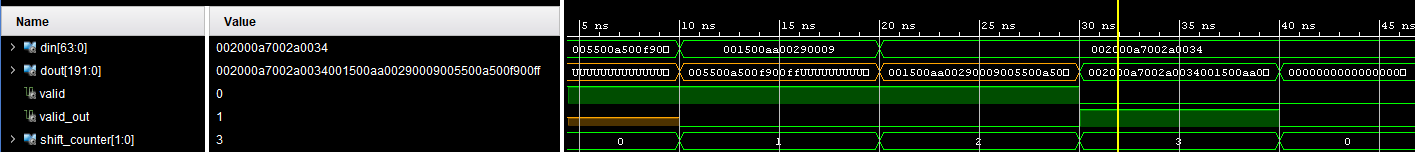
\includegraphics[scale=0.45]{images/simulation_results/shiftregister_p_bands_12.PNG}}
  \caption{simulation of \textbf{Shiftregister} for $P\_bands$ = 12. } 
  \label{fig:simulation_shiftregister}
\end{figure}
 
 \subsection{ACAD correlation}

 Constrained random input simulation of \textbf{ACAD correlation} has been done in Vivado, and the captured waveforms has been visually inspected. The waveforms shown in Figure \ref{fig:simulation_results_correlation_one} and \ref{fig:simulation_results_correlation_two} shows simulations of input pixel vectors of size $P\_bands$ =4, $Pixel\_data\_width$ =16.\\
 
 Figure \ref{fig:simulation_results_correlation_one} shows a simulation for a data input pixel vector of [0x00ff, 0x00f9, 0x00a5, 0x0055]. This is simulated to be the first pixel of the hyperspectral image.\\
 
 Figure \ref{fig:simulation_results_correlation_one} shows a simulation for a data input pixel vector of [0x0015, 0x00aa, 0x0029, 0x0009]. This is simulated to be the second pixel of the hyperspectral image.
 
 



\begin{figure}[H]
\refstepcounter{figure}
\begin{tabular}{c|c}

   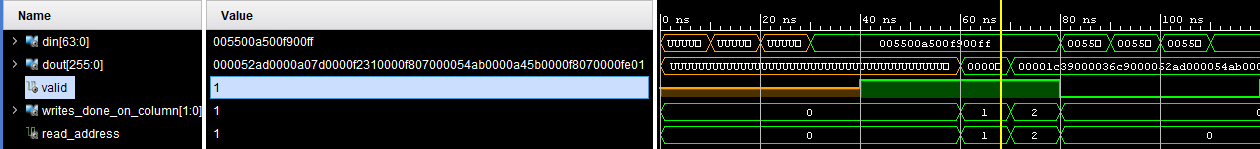
\includegraphics[scale=0.6, angle=90, origin=c]{images/simulation_results/correlation_pixel_one.PNG}
   \rotatebox[origin=c]{90}{ Figure~\thefigure: Simulation of the \textbf{ACAD correlation} block.}
  %\caption{ \textbf{ROTATE}FSM controlling the architecture shown in Figure  } 
  \end{tabular}
  \label{fig:simulation_results_correlation_one}
\end{figure}


\begin{figure}[H]
\refstepcounter{figure}
\begin{tabular}{c|c}

   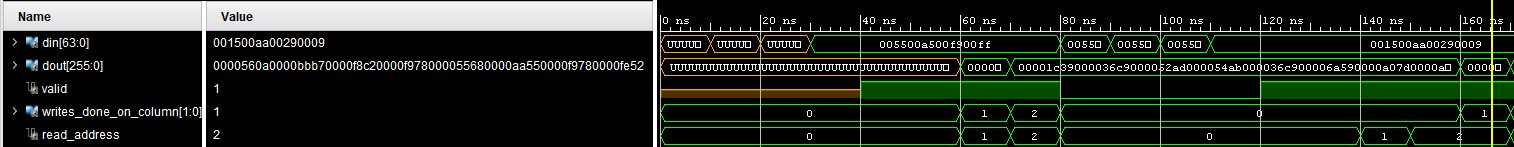
\includegraphics[scale=0.5, angle=90, origin=c]{images/simulation_results/correlation_pixel_two.PNG}
   \rotatebox[origin=c]{90}{ Figure~\thefigure: Simulation of the \textbf{ACAD correlation} block.}
  %\caption{ \textbf{ROTATE}FSM controlling the architecture shown in Figure  } 
  \end{tabular}
  \label{fig:simulation_results_correlation_two}
\end{figure}


 
 \subsection{Inverse}
 Simulation has been done with $P\_bands$=[4,6] and $Pixel\_data\_width$= 16, with constrained random input.  Figure \ref{fig:simulation_results_inverse} shows a simulation with $P\_bands$ = 4.   


\begin{figure}[H]
\refstepcounter{figure}
\begin{tabular}{c|c}

   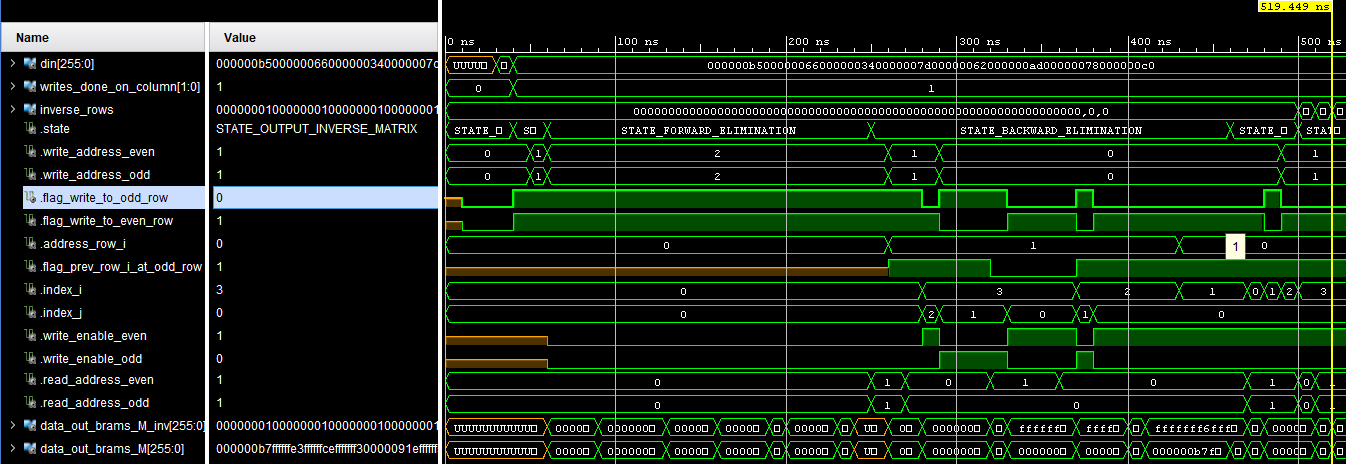
\includegraphics[scale=0.6, angle=90, origin=c]{images/simulation_results/complete_inverse_bram_approach_4_by_4_matrix_formatted_for_latex.png}
   \rotatebox[origin=c]{90}{ Figure~\thefigure: Simulation of the \textbf{Inverse} block.}
  %\caption{ \textbf{ROTATE}FSM controlling the architecture shown in Figure  } 
  \end{tabular}
  \label{fig:simulation_results_inverse}
\end{figure}


\chapter{Discussion}
\label{sec:Discussion}

\section{Resource usage}
\subsection{DSP usage $Pixel\_data\_width$ = 16}
Synthesis results shows that \textbf{ACAD correlation} infers $P\_bands$ $\times$ 4 DSP48E1s and $P\_bands$ BRAMs for $Pixel\_data\_width$ = 16. \\


\\
The \textbf{ACAD inverse} using the LUT-approach also infers a large number of DSPs. The Zynq Z-7030 contains 400 DSP Slices, while the Z-7035 contains 900. According to synthesis results the LUT-approach implementation of the \textbf{Inverse} block utilizes 540 DSPs for $P\_bands$ = 30 and $Div\_Precision$ = 17. As \textbf{ACAD correlation} infers $P\_bands$ $\times$ 4 DSPs for $Pixel\_data\_width$ >= 11, the total number of DSPs synthesized for these two modules for $P\_bands$ and $Div\_Precision$ =16 will be 660. This is a lot, especially considering that \textbf{dACAD} computes $\delta^{ACAD}(\textbf{x}_k)= \textbf{x}_k^T\Tilde{\textbf{R}}^{-1}(\textbf{x}_k)\textbf{x}_k$, in which $\textbf{x}_k$ is a pixel vector of size $P\_bands$ $\times$ $Pixel\_data\_width$, and $\Tilde{\textbf{R}}^{-1}(\textbf{x}_k)$ is a matrix of size $P\_bands$ $\times$ $P\_bands$ $\times$ $Pixel\_data\_width$. This computation will most likely also utilize DSPs, depending upon implementation.  
The large usage of DSPs constrains the size of the matrix possible to input to the ACAD AD. %If $Pixel\_data\_width$ = 16, this means  
% Solution; correlation; spend more time ? HALF the amount of DSPs, doubling the time?
\subsection{$Pixel\_data\_width$ = 10}
When synthesizing \textbf{ACAD correlation} with $Pixel\_data\_width$ = 10 no DSPs are inferred. Instead the logic gets mapped to LUTs as shown in Figure \ref{fig:correlation_luts_and_registers_10}. Inferring the logic in LUTs instead of in DSPs leads to the design failing to meet timing, as shown in Table \ref{tab:wns_correlation_10}. But, as can also be observed Table \ref{tab:wns_correlation_10}, the \textbf{Net delay} is high, and increasing as a function of $P\_bands$. This is due to the output ports of \textbf{ACAD correlation} getting mapped to physical output pins on the synthesized device. This will not be the case in implementation, as the output ports of \textbf{ACAD correlation} is proposed connected to \textbf{ACAD inverse} and \textbf{FSM ACAD}. 
As such, the net delay is most likely unrealistically large, as mapping to output pins scattered on the physical interface of the device will result in higher delay than mapping to internal buses located inside the device. It is therefore the authors belief that \textbf{ACAD correlation} will meet timing once the design is a submodule of the ACAD anomaly detector.  



\section{Timing results}
\textbf{Correlation}

The 

\subsection{\textbf{Inverse}}
 Implementing division using the division operator "/" is not viable, as the \textbf{Last division} block fails to meet timing requirements when using this approach. This holds for dividend/divisor bit width down to five. \\

The adaptive shifting approach is an interesting approach for implementation of division, and the approach meets timing requirements. A large uncertainty however, is the effect of precision error when utilizing this approach.\\ 

Implementing division through the LUT-approach shows promising results with regards to timing. The author has not focused on optimizing the LUT-approach with regards to timing, as the approach was implemented late in the process of doing this thesis. The synthesis results for the \textbf{Inverse} block when using LUT-approach with $Div\_Precision$ =17 yielded a WNS of -5.972ns, in which 4.847 of this is net delay. This net delay is most likely unrealistic large, as the outputs of the \textbf{Inverse} block is mapped to output pins when running synthesis using the \textbf{Inverse} block as top module. This will not be the case for the complete implementation of the ACAD anomaly detector, as the output from the \textbf{Inverse} module will be mapped to an internal bus connected to the \textbf{dACAD} block. The net delay will therefore be considerably lower.  The additional -1.25 ns WNS owing to logic delay may be reduced when running implementation instead of synthesis, as implementation results typically reduce number of LUTs inferred.  \\
\newpage
\chapter{Conclusion}
\label{sec:conclusion}


%%Future Work
%Future of FPGAs? Scaling, Moores law...
%MCU\\
%Battery-technology?\\
%Lumen -measurement on chip?(For image processing)\\

%Are your results satisfactory?\\
%Can they be improved?\\
%Is there a need for improvement?\\
%Are other approaches worth trying out?\\
%Will some restriction be lifted?\\
%Will you save the world with your Nifty Gadget?++
%

\section{Future work}

\subsection{Optimizations}

All BRAMs used in the correlation module could have its content initialized to zero. This could help simplify the control of the correlation module.

\\ 
Evaluate the value $\tau$ based on experimental results.\\

Inverse computation; use Matrix Inversion Lemma as proposed by Hsueh in \cite{hsueh_master_thesis}.\\

Power optimizations; clock enable signals for modules.\\

Precision LUT approach must be checked!\\

Verificiation!!!






%\input{Sections/example}
% Bibliography - edit references.bib and use the \cite command in text
\newpage
\bibliographystyle{IEEEtran}
\bibliography{references}
\begin{appendices}
\newpage
\chapter{MATLAB hyperspectral}
\label{appendice:MATLAB_hyperspectral} %
\end{appendices}

\end{document}
